\documentclass{thesis}

\usepackage[dutch,english]{babel}

\usepackage[svgnames]{xcolor}
\definecolor{papergray}{HTML}{34495e}
\definecolor{paperblue}{HTML}{3498db}
\definecolor{lightgray}{gray}{0.9}

\usepackage{graphicx, booktabs, rotating, subfigure, 
            array, parallel, csquotes, colortbl, 
            makeidx, tabularx, amsmath, tikz
}

\usepackage[super]{nth}
\usetikzlibrary{decorations.text}

\usepackage[notes,natbib,maxcitenames=2]{biblatex-chicago}
\addbibresource{main.bib}

\usepackage[hang,flushmargin,norule,bottom,multiple]{footmisc} 

\makeatletter
\renewcommand\@makefntext[1]{% 
    \@thefnmark.~#1}
\makeatother

\DefineBibliographyStrings{english}{%
  references = {\uppersf{Bibliography}},
}

\newcommand*{\oldstyle}{\normalsize\fontfamily{bch}\selectfont}
\newcommand*{\intstyle}{\normalsize\bf\fontfamily{ppl}\selectfont}
\newcommand*{\newstyle}{\normalsize\fontfamily{phv}\selectfont}

\newcommand*{\argmin}{\operatornamewithlimits{arg\,min}\limits}
\newcommand*{\argmax}{\operatornamewithlimits{arg\,max}\limits}
\DeclareMathOperator*{\argsort}{arg\,sort}

% new commands
\usepackage{mathtools,dcolumn}
\newcommand\p[1]{\phantom{#1}}
\newcommand\dnum[1]{%
    \begin{tabular}{@{}D{.}{.}{3.1}@{}}
      #1
    \end{tabular}}

% document details
\author{Folgert Karsdorp}
\title{Retelling Stories}
\date{}

\begin{document}
\frontmatter
\raggedbottom
%!TEX root = main.tex


{       \centering
        \vspace*{1cm}
        
        {\sffamily\lsstyle\LARGE R\reflectbox{E}TELLING STORIES}\\\vspace{1.5cm}
        {\sffamily\lsstyle\Large A COMPUTATIONAL- \vspace{0.5cm}\\EVOLUTIONARY PERSPECTIVE}\\\vspace{1.5cm}
        {\sffamily\lsstyle\normalsize FOLGERT KARSDORP}
        
        \vfill           
          \thispagestyle{empty}%
          \clearpage
}          

%!TEX root = ../main.tex
\vspace*{\fill}
\thispagestyle{empty}%
\noindent Cover design by Basten Stokhuyzen (\url{http://www.bstn.nl/})\vspace{0.1cm}\\
ISBN 978-90-9029993-8\vspace{0.1cm}\\
\textcopyright\ 2016, Folgert Karsdorp\vspace{0.1cm}\\
Published under the terms of the Creative Commons Attribution License, CC BY 4.0 (\url{http://creativecommons.org/licenses/by/4.0/}), which permits unrestricted use, provided the original author and source are credited.
\clearpage
%!TEX root = ../main.tex


\begin{titlepage}
        \centering
        \vspace*{1cm}
        
        {\sffamily\lsstyle\LARGE R\reflectbox{E}TELLING STORIES}\\\vspace{1.5cm}
        {\sffamily\lsstyle\large A COMPUTATIONAL- \vspace{0.5cm}\\EVOLUTIONARY PERSPECTIVE}\\\vspace{1.5cm}

        {Proefschrift ter verkrijging van de graad van doctor \\
         aan de Radboud Universiteit Nijmegen \\
         op gezag van de rector magnificus prof.\ dr.\ J.H.J.M.\ van Krieken, \\
         volgens besluit van het college van decanen \\
         in het openbaar te verdedigen op \\\vspace{0.5cm} }

         {dinsdag 6 december 2016} \\\vspace{0.5cm}

         {om 12:30 uur precies} \\\vspace{0.5cm}

         {door} \\\vspace{0.5cm}

         {Folgert Bastiaan Karsdorp} \\\vspace{0.5cm}

         {geboren op 3 november 1983} \\\vspace{0.5cm}

         {te Leidschendam} \\\vspace{1.5cm}
        
        \vfill           
          \thispagestyle{empty}%
          \clearpage%         
\end{titlepage}
%!TEX root = ../main.tex

{\filcenter
  {\sffamily\lsstyle\MakeUppercase{Promotoren}}\\\vspace{0.667\baselineskip}
    Prof.\ dr.\ Antal van den Bosch\\\vspace{0.2cm}
    Prof.\ dr.\ Franciska de Jong (Erasmus Universiteit Rotterdam; Universiteit Twente; Universiteit Utrecht)\\

  \vspace{2\baselineskip}  
  {\sffamily\lsstyle\MakeUppercase{Copromotoren}}\\\vspace{0.667\baselineskip}
    Prof.\ dr.\ Theo Meder (Meertens Instituut, Amsterdam; Rijksuniversiteit Groningen)\\\vspace{0.2cm}
    Dr.\ Peter van Kranenburg (Meertens Instituut, Amsterdam)\\

  \vspace{2\baselineskip}
  {\sffamily\lsstyle\MakeUppercase{Manuscriptcommissie}}\\\vspace{0.667\baselineskip}
    Prof.\ dr.\ Margot van Mulken\\\vspace{0.2cm}
    Prof.\ dr.\ Karina van Dalen-Oskam (Universiteit van Amsterdam; Huygens ING, Amsterdam)\\\vspace{0.2cm}
    Prof.\ dr.\ Tim Tangherlini (University of California,\\Los Angeles, Verenigde Staten)\\\vspace{0.2cm}
    Prof.\ dr.\ Helma van Lierop (Tilburg University)\\\vspace{0.2cm}
    Dr.\ Ben Miller (Georgia State University, Atlanta, Verenigde Staten)\\
}
      
\thispagestyle{empty}%
\clearpage%
\cleardoublepage
%!TEX root = ../main.tex

\clearpage     
\thispagestyle{empty}
\vspace*{\stretch{2}}
\chapterprecishere{\large
  It gets easier. Every day it gets a little easier. But you got to do it every day. That's the hard part. But it does get easier.}{Bojack Horseman}{\large Out to Sea}
\vspace*{\stretch{3}}
\clearpage

\setcounter{tocdepth}{0}
\tableofcontents

%!TEX root = ../main.tex

\chapter*{Acknowledgments}
\addcontentsline{toc}{chapter}{Acknowledgments} \markboth{ACKNOWLEDGMENTS}{} \markright{ACKNOWLEDGMENTS}

\noindent Any story is shaped by the stories that surround it. This dissertation is no different. It could not have been told without the stories of all the wonderful people that have supported me during the past four and a half years. 

First and foremost, I would like to thank my supervisor Prof.\ dr.\ Antal van den Bosch. During my MA training, I read Antal's book on memory-based learning, which was a paradigm-shifting experience. It sparkled my interest in pursuing a Ph.D with a component in language technology. I was very fortunate to be offered a Ph.D position in the Tunes \& Tales project, which not only allowed me to expand my knowledge about computational language modeling, but also to learn it from the best. Antal has my deepest gratitude for all his guidance, intellectual encouragement and much-needed advice on presentations, articles, grant proposals, job positions, and different revisions of the manuscript. 

I thank my second supervisor Prof.\ dr.\ Franciska de Jong for shepherding the manuscript through its final stages. Furthermore, I am grateful to my two co-promotors, Prof.\ dr.\ Theo Meder and Dr.\ Peter van Kranenburg, from whom I benefited immeasurably. Both Theo's profound knowledge of folktales and oral culture, and Peter's invaluable suggestions at numerous occasions have improved the quality of this dissertation considerably. 

A number of colleagues at the Meertens Instituut have been generous with their time and expertise: Berit Janssen, Marianne van Zuijlen, Dong Nguyen, Dolf Trieschnigg, and Iwe Muiser. The embedding of the Tunes \& Tales project within the eHumanities group of the Royal Dutch Academy of Arts and Sciences has given me the opportunity to engage in interesting discussions regarding the emerging field of Digital Humanities, and I wish to thank Prof.\ dr.\ Sally Wyatt, Dr.\ Andrea Scharnhorst, Jeannette Haagsma, and Anja de Haas-Gruys for all their effort and time. Finally, I thank the LAMA's of the Radboud University for encouraging me to leave Amsterdam once in a while.

I am enduringly grateful to my friends and family for their emotional support, patience and  encouragement. I single out three close friends, whom I owe special thanks. First, I thank Basten Stokhuyzen, who implemented the front-end of MOMFER, designed the wonderful cover of this dissertation, and proved to be a steady friend. I am also greatly indebted to Marten van der Meulen, who has been been my research assistant for approximately two years, has co-authored and co-presented several of my articles, and is one of the smartest and funniest persons I know. This dissertation has benefited repeatedly from Marten's wise and thoughtful suggestions, as well as from his enduring patience regarding my endless stream of trial projects. Finally, I thank Lauren Fonteyn, who has been an incisive reader and patient editor of different drafts of this dissertation. Without Lauren's intellectual breadth, critical judgment, and inspiring companionship, I doubt whether this dissertation had been completed at all.

\mainmatter
%!TEX root = ../main.tex

\chapter{Introduction}\markboth{INTRODUCTION}{} \markright{INTRODUCTION}\label{ch:introduction}

\chapterprecishere{``To explain culture, then, is to explain why and how some ideas happen to be contagious.''}{Dan Sperber}{Explaining Culture}

\vspace{3.5ex plus 1ex minus .2ex}
\noindent This study examines the mechanisms underlying the selection and transmission of stories from an evolutionary perspective. Stories, much like human beings, have lives, which start the moment a particular event or experience is formulated in narrative form. Their further `survival' crucially depends on their being re-told: a story that does not acquire new tellers ``can have no life beyond the life of the original person who experienced the events and first formulated them as a story''\autocite{linde:2009}. By being transmitted from one individual to another, stories may propagate, sometimes from generation to generation. Some stories propagate so effectively -- or, to use Sperber's wording, `contagiously' -- that they become part of a culture's central heritage. 

When stories are propagated, they tend to get altered and reshaped with each retelling. Experimental studies on story transmission have shown that factors such as memory capacity and other social-cognitive pressures can have severe impact on how accurately stories are transmitted.\autocite{bartlett,mesoudiwhiten:2010,breithaupt:2015} In other words, stories are commonly subjected to `imperfect replication', and, as such, their transmission leads to their gradual transformation. Interestingly, while such experimental studies merely regard the reshaping of stories as a natural by-product of their being transmitted by multiple agents, some critics have argued that reshaping or transformation is in fact an essential prerequisite for a story's survival; a story \emph{needs} to be recurrently adapted to secure its position in culture\autocite{stephens_mccallum,collins_ridgman}. As \citeauthor{geerts_bossche} state: ``Without all of the transformations, which keep the work available, it would no longer be read and therefore `die out'''.\autocite{geerts_bossche} The fact that stories need to be altered to survive even seems to be the case for fairy tales, some of which are among the most `contagious' stories in present-day Western culture (e.g.\ ``Cinderella'' and ``Snow White''). Notwithstanding the fact that many fairy tales have been kept in relatively stable form for centuries (at least on an abstract, structural level), the current study wishes to argue that even fairy tales undergo progressive alterations as the result of a process of modification in which changes are gradually accumulated.

Although the complex interplay between adaptation and selection in story transmission has been recognized by various scholars in literary and folklore studies\autocite[E.g.][]{boyd:2009,zipes:2006,zipes:2012,sanders:2006,hutcheon:2013}, these claims are, unfortunately, largely programmatic: the current accounts of adaptation and selection in story transmission posit thought-provoking theoretical claims, but they do not systematically nor quantitatively test these claims. Thus, if we wish to arrive at a more concrete and precise understanding of the selection forces that underlie the transmission of stories, we are faced with a challenge: we need to suggest and develop new ways to empirically and quantitatively verify such programmatic claims.

With the current study, I aim to tackle this challenge by drawing inspiration from the cultural evolution research program\autocite{sforzafeldman:1981,boyd_richerson:1985,mesoudi:2011}. This program aims to enhance our understanding of cultural selection processes by means of formal models of cultural evolution, which allow us to quantitatively assess changes in cultural variation over time. In recent years, special attention has been devoted to a neutral model of cultural evolution which is comparable to biological drift. In this neutral model, individuals either introduce new variants of a particular cultural trait to the population or copy existing variants proportionally to the frequency of these variants in the population, and more popular variants are more likely to get adopted than less popular ones. This simple model accurately predicts a variety of cultural evolutionary processes, such as the selection of keywords in academic publications\autocite{Bentley:2008}, the choice of baby names\autocite{Hahn:2003}, and the popularity of particular dog breeds\autocite{herzog:2004,ghirlanda:2014}. This random copying model, strikingly, appears to be so accurate that researchers consider it to be the null hypothesis in the description of cultural evolutionary processes. Put differently, it is held that cultural evolution proceeds randomly, unless proven otherwise. Formal models of cultural evolution have at least three major advantages over the programmatic statements that are often employed in literary and folklore studies, which are often based on intuition or research on a small corpus. First, to explain prevalent culture, formal models call for detailed and replicable descriptions and definitions of the mechanisms and processes that underlie cultural change. Second, by adopting a formal approach, researchers can attempt to isolate and systematically compare forces of selection. Finally, one of the most important characteristics of quantitative, computational models is that they yield specific predictions that can be tested experimentally or against observations in real-world data\autocite[For an elaborate discussion, see][]{mesoudi:2011}.

The predictions made by quantitative models, such as, for instance, those built by \citeauthor{sforzafeldman:1981}\autocite{sforzafeldman:1981}, have been supported by experimental studies of story transmission. In several of these studies, story transmission is experimentally simulated by means of a `transmission chain' method, which closely resembles the game called `Chinese whispers' or `telephone' in the United States.\autocite{bartlett,mesoudiwhiten:2008} In these transmission simulations, participants attempt to memorize a story from either reading or listening and pass on their version of the story to the next participant generation. An interesting example of such an experimental study is the one by \citeauthor{eriksson:2012} who describe an inhibiting effect of multiple `parents' in transmission chains (i.e.\ chains in which stories are retold on the basis of more than one previous version) on the rate at which stories change.\autocite{eriksson:2012} Although experimental studies such as these have yielded a wealth of insights about underlying mechanisms of story transmission, a striking lack in cross-disciplinary communication and exchange of information with literary and folklore research prevents these insights to find their way across fields. Additionally, experimental story transmission studies have focused primarily on finding explanations for the progressive alterations of stories, and not on determinants of binary selection\autocite[Notable exceptions include, e.g.][]{Heath:2001,eriksson:2014}. Put differently, while story transmission studies mainly seek to map out how one and the same story changes through transmission, they do not explain why a story — or in some cases a group or `assemblage' of stories — is recurrently retold and becomes successful, whereas others go extinct altogether.\autocite{zipes:2006,zipes:2012} As such, it remains unclear how experimental results should be interpreted in light of real-world story transmission and selection.

One of the main obstacles to study the phenomena observed in real-world story transmission processes is the lack of detailed historical data that specifies the exact paths of transmission between different individuals and generations. The task of identifying such paths of story transmission would be easier to accomplish with diachronic data that describes who learns or copies from whom\autocite{kandler:2015}. Unfortunately, although a number of folktale digitization initiatives which provide large-scale collections of folktales have been undertaken recently\autocite{abello:2012,barre:2012,meder:2010,meder:2016}, longitudinal data collections of real-world stories are still virtually non-existent. The current study aims to meet this demand by delivering a large diachronic collection of Dutch versions of the fairy tale ``Little Red Riding Hood''.

The central question of this study is whether story transmission can be understood and hence should be described as a cultural evolutionary process, and, if so, which evolutionary mechanisms can be identified in story transmission processes. The main focus of the study are the mechanisms that underlie story transmission processes in folktales. Additionally, the goal is to unite the study's findings, whether they are in line with or contrary to the predictions of evolutionary models, with existing literary and folklore accounts of story transmission and selection. As such, this study contributes to the further synthesis of the disciplines of cultural evolution, literature and folklore. The research's relevance ranges from providing answers to methodological questions regarding how and to what extent evolutionary mechanisms underlying real-world story transmission can be studied from real-world, historical corpus data, to offering more abstract, theoretical reflections on pre-textual relations between stories. In particular, I will address the following four research questions:
\begin{description}
\item[Research question 1:] How should stories be formally represented in order to study real-world story transmission and selection with computational means?
\item[Research question 2:] Can historical corpus data be employed to reveal content biases in story transmission?
\item[Research question 3:] Can we describe the diachronic development of stories as a gradual accumulation of modifications and hence as an evolutionary process?
\item[Research question 4:] Can story transmission and selection be described as a random selection process, and what other mechanisms underlying story transmission and selection can be discerned from historical corpus data?
\end{description}
Research question 1 serves as the methodological base to further investigate the other questions. In the present study, I experiment with a number of different representations of stories, which all have potential advantages and disadvantages for studying story transmission. In particular, I consider the following representations: (i) motif representations (Chapter \ref{ch:motif-classification}), (ii) semantic representations of the character cast of stories (Chapter \ref{ch:animacy}), (iii) representations based on manual narratological text analysis (Chapter \ref{chp:red-riding-hood}), and (iv) `bag-of-words' representations (Chapter \ref{ch:story-networks}). 

In folktale research, the relations between stories are often investigated by means of motif representations. Motifs, such as those found in the \emph{Motif-Index} by Stith Thompson\autocite{thompson:1955}, are considered to be the primary building blocks of stories and their constellation defines the tale type of a story as categorized in folktale catalogs such as \emph{The Types of International Folktales}\autocite{uther:2004}. The current study wishes to contribute to these folklorists' research endeavors by delivering two research instruments which allow researches to analyze large-scale folktale collections and the relations between folktales in terms of their motifs more efficiently. 

The first research instrument is aimed at making existing collections of folklore motifs more accessible. To this end, more than fifty years after the first edition of Thompson's seminal \emph{Motif-Index of Folk Literature}, I present an online search engine in Chapter \ref{ch:motif-classification}, which is tailored to fully disclose the index digitally. This search engine, called \index{MOMFER}MOMFER, greatly enhances the searchability of the \emph{Motif-Index} and provides exciting new ways to explore the collection. This is enabled by the use of modern techniques from the fields of Natural Language Processing and Information Retrieval. The key feature of the search tool is the way in which it allows users to search the \emph{Motif-Index} for semantic concepts, such as `mythical animals', `mortality', or `emotions'. In the first part of Chapter \ref{ch:motif-classification}, I will explain the motivations for creating the search tool, lay bare its production process, and show in a number of case studies how the search tool can be used to explore the index in innovative ways. The second part of Chapter \ref{ch:motif-classification} presents an automated motif identification system. This second research instrument enables scholars to efficiently identify motifs in large-scale folktale collections as well as the relations between stories in terms of their motif representations.

Chapters \ref{ch:animacy}, \ref{chp:red-riding-hood}, and \ref{ch:story-networks} more directly address the evolutionary questions of this study. Chapter \ref{ch:animacy} aims to further our knowledge about how to explain prevalent culture, in which cultural artifacts are differentially preferred and some artifacts are more likely to survive than others. As a case study, I systematically examine the cultural successfulness of fairy tales from the Brothers Grimm collection \emph{Kinder- und Hausmärchen} from a \emph{content}-based perspective (research question 2). I address of which story elements contribute to a story's popularity (or, in other words, which story elements form attractors causing a fairy tale to `stick' and gain popularity). In particular, I look into the question whether the type of characters in a story correlates with its successfulness, i.e.\ whether a character type bias is at play in story selection. An essential methodological prerequisite for addressing this question is to find a way to list the character cast of a story. To this end, I first present a linguistically uninformed computational model for animacy classification with which characters can be automatically identified in folktales. I compare the model to a number of linguistically \emph{informed} models that use features such as dependency tags, and show competitive results. The animacy classifier serves as the methodological base to further investigate the question of whether the cultural success of fairy tales can be (partially) ascribed to character type biases. I apply the animacy classifier to a large collection of Dutch folktales, to develop a typology of character types. By mapping the character casts of a selection of successful and unsuccessful fairy tales from \emph{Kinder- und Hausmärchen} to this typology, I provide empirical evidence for several character types that discriminate between successful and unsuccessful tales.

The remaining two chapters (\ref{chp:red-riding-hood} and \ref{ch:story-networks}) focus on socially informed, \emph{context}-based processes that underlie story transmission and selection. Chapter \ref{chp:red-riding-hood} aims to enhance the understanding of the processes through which stories for children are retold. The study addresses the third research question of this thesis and investigates whether the diachronic development of the world's most famous fairy tale ``Red Riding Hood'' is to be characterized as a process of gradual accumulation of modification, with new variants of the story most likely deriving from previous versions in temporal proximity. Results suggest that new Dutch versions of ``Red Riding Hood'' are potentially subjected to age-dependent selection processes (i.e.\ fashion trends or fads), which means that `young' story versions are preferred in producing a new version. The analysis presented here is based on a digitized collection of Dutch ``Red Riding Hood'' retellings\autocite{folgert_karsdorp_2016_51588}. This collection forms the largest longitudinal collection of children's stories today and holds a wealth of information for studies in (children's) literature, history, sociology, folklore, linguistics, and cultural evolution. 

Finally, further building upon insights and experimental results from Chapter \ref{chp:red-riding-hood}, I pursue a more detailed understanding of the processes through which stories are retold in Chapter \ref{ch:story-networks} (research question 4). A collection of story retellings can be considered as a network of stories, in which links between stories represent pre-textual (or ancestral) relationships. In this chapter, I provide a mechanistic understanding of the structure and evolution of such story networks. I construct story networks for two diachronic story collections: (i) the collection of Dutch ``Red Riding Hood'' retellings from Chapter \ref{chp:red-riding-hood} and (ii) a corpus of paper chain letters. The results confirm and strengthen the analysis presented in Chapter \ref{chp:red-riding-hood} by showing that the formation of these story networks is guided by age-dependent selection processes. Subsequently, I systematically compare these findings with and among predictions of various formal models of network growth to determine more precisely which kinds of attractiveness are also at play or might even be preferred as explicatory models. Carefully studying the structure and evolution of the two story networks, I show that existing stories are differentially preferred to function as a new version's pre-text given three types of attractiveness: (i) frequency-based and (ii) model-based attractiveness which (iii) decays over time.

Earlier versions of parts of this thesis have appeared as journal articles and papers in conference proceedings. Although much of this material has been substantively extended and revised for the current study, I feel that a study about story transmission should at least make its sources explicit:

\begin{refsection}
\nocite{karsdorp:2012,karsdorp:2012b,karsdorp:2013,Karsdorp:2013tk,karsdorp:2015a,karsdorp:2015b,karsdorp:story-networks,folgert_karsdorp_2016_51588} % karsdorp:retelling
\printbibliography[heading=none, keyword=mywork]
\end{refsection}
%!TEX root = ../main.tex

\chapter{Motif Annotation \& Classification}\label{ch:motif-classification}

\chapterprecishere{``A motif is the smallest element in a tale having a power to persist in tradition.''}{Stith Thompson}{The Folktale}

\section{Introduction}

In the introduction to his seminal \emph{Motif-Index of Folk Literature} (TMI), Stith Thompson addressed a number of fundamental challenges in folklore research. One crucial problem concerns ``the need for a comprehensive classification of the materials in all kinds of traditional narrative''\autocite[8]{thompson:1955}, which became all the more urgent in light of the ever-growing number of tales that were being collected at the time. Furthermore, he felt that the then current type index by Antti Aarne\autocite{aarne:1928} was not sufficient for indexing folktales from outside Europe. Thompson took it upon himself to try to remedy this situation by classifying folktales on the basis of motifs, which resulted in the first edition of the TMI in the 1930s\autocite{thompson:1932} and a revised and enlarged second edition in the 1950s that nearly doubled its scope\autocite{thompson:1955}.

In folktale research, motifs are a key concept in the classification of folktales into tale types. In the authoritative folktale type catalog, \emph{The Types of International Folktales}\autocite{uther:2004} -- a project initiated by Aarne in 1910 in his \emph{Verzeichnis der Märchentypen} (Catalogue of tale types)\autocite{aarne:1910}, which was translated and revised by Thompson\autocite{aarne:1928,aarne:1961} -- motifs form the primary descriptive units, and their configuration defines the folktale type of a story. There is, however, a large body of criticism aimed at the TMI as well as the different editions of the folktale type index, such as, for example, \citeauthor{dundes:1997} in relation to Aarne's 1961 edition\autocite{dundes:1997}, and \citeauthor{karsdorp:2012} with respect to Uther's most recent edition of the \emph{The Types of International Folktales}\autocite{karsdorp:2012}. This criticism has focused on the distribution and overlap of tale types and motifs. Furthermore, \citeauthor{el-shamy:1980} addresses the lacunae in the collection of sources used\autocite{el-shamy:1980}. Despite the various problems with respect to the applicability of the Aarne/Thompson folktale index to non-European tales, El-Shamy states that ``these can be adequately addressed through its [the folktale index's] relatively open classification system, which allows for adding new items, particularly when compared to other systems''\autocite[158]{el-shamy:1988}. Additionally, Alan Dundes states:
\begin{quote}
    It must be said at the outset that the six-volume \emph{Motif-Index of Folk-Literature} and the Aarne-Thompson tale type index constitute two of the most valuable tools in the professional folklorist's arsenal of aids for analysis. This is so regardless of any legitimate criticisms of these two remarkable indices, the use of which serves to distinguish scholarly studies of folk narrative from those carried out by a host of amateurs and dilettantes. The identification of folk narratives through motif and/or tale type numbers has become an international \emph{sine qua non} among bona fide folklorists.\autocite[195]{dundes:1997}
\end{quote}
While many new motif indices\autocite[See e.g.][]{baughman:1966,ideka:1971,kirtley:1977,childers:1977,flowers:1980,neuland:1981,el-shamy:1995} as well as many new collections of folktales\autocite{el-shamy:1980,meder:2000,slone:2001,crooke:2002} have since been put forward, relatively few attempts have been made to combine the two\autocites[Although see, in recent years][]{ben-amons:2006,slone:2001}[For further examples of both motif indices as well as folktale collections, see][]{uther:1996}. I hypothesize that the lack of combining the two resources is related to a lack of navigability of the TMI. Furthermore, while many of the researchers explicitly integrate their new indices into the TMI\autocite[For a brief and recent example, see][]{bell:2009}, there is no complete and combined edition of all these indices. Because of the problems that printing a book of such magnitude would generate, it is understandable that such an edition is unavailable. These considerations would evaporate for a digital edition. Yet, however valuable a research tool it would be, no digital edition exists at present. Given the TMI's unquestioned status as \emph{the} source for the worldwide coverage of folk narrative, a search engine of the TMI would be of interest to many scholars, ranging from folklorists to narratologists and story generation researchers.

The aims of the present chapter are the following. First, I wish to highlight some of the navigational challenges one has to overcome in order to make use of existing motif indices successfully, taking the TMI as a case study. I agree with Harriet Goldberg that ``[t]he utility of an index of folk-motifs clearly lies in its ability to present in an orderly framework those transitory flashes of recognition that we experience upon hearing a familiar story or a familiar narrative component in a new context''\autocite[xiii]{goldberg:1998}. To meet this objective, I present \emph{Meertens Online Motif FindER} (MOMFER), which is a free, online search engine designed to increase the accessibility of the TMI.\footnote{Available at \url{http://www.momfer.ml}} This tool provides various new and unique access points to the index, drawing inspiration from techniques used in the fields of Natural Language Processing and Information Retrieval.\autocite[For a similar approach that attempts to enrich the motif index with semantic information, cf.][]{declerck:2011} MOMFER enables several different search options: besides basic options such as single word, multi-word, and phrase searches, it is also possible to use faceted search, and even semantic search. These options, I suggest, can provide new tools for researchers and can lead to the asking and answering of questions that were hitherto deemed unanswerable. Furthermore, there is great potential for this tool to be used as a framework into which all other existing motif indices will be integrated.

Second, one is confronted with the problem that, although the motif search engine MOMFER provides researchers with a indispensable research tool to more efficiently access and retrieve information from the TMI, it remains rather cumbersome and time-consuming to manually label folktales with their corresponding motifs. This is especially the case in large-scale collections such as the Dutch Folktale Database.\autocite{meder:2010,meder:2016} In order to reduce the amount of manual labor, then, I will develop a computational system with which motifs can be automatically assigned to folktales. If this automated motif classification system is combined with MOMFER, the analysis of large-scale folktale collections is greatly facilitated, which will aid and enhance future research aimed at mapping out relations between stories and their motifs.

The present chapter is structured as follows: first, I will briefly introduce the TMI to those readers who may be unfamiliar with it, which is followed by a discussion of some important navigational challenges associated with its use (Section \ref{sec:momfer-accessibility}). Subsequently, I will describe the creation process and architecture of MOMFER (Section \ref{sec:momfer-production}), after which I will proceed to highlight a number of interesting search options by presenting several case studies that use the TMI as a corpus (Section \ref{sec:momfer-case-studies}). The second part of this chapter is devoted to the development of the automated system for motif identification (Section \ref{sec:motif-classification}). 

\section{MOMFER}

\subsection{Accessibility of the \emph{Motif-Index}}\label{sec:momfer-accessibility}

The TMI\autocite{thompson:1955} contains over forty-five thousand motifs spread out over five volumes. The motifs are hierarchically ordered in a tree structure. There are twenty-three top-level, alphabetically labeled categories, whose contents range from mythological motifs (Category A) to motifs concerning traits of character (Category W) and beyond. Each top-level category is divided into various subcategories: for example, Category D (\emph{Magic}) is divided into, inter alia, \emph{Transformation} (D0--D699) and \emph{Magic Objects} (D800--D1699), which in turn branch out into child motifs, and so on and so forth. At the leaves of the tree, or terminal nodes, we find the most specific instances of a particular motif\autocites[For an elaboration on the build-up of the index and search strategies, see][Volume 1, 19–25]{thompson:1955}[16--17]{el-shamy:1995}. Figure \ref{fig:thompson-tree} is an exemplary representation of part of the hierarchical tree.

\begin{figure}
    \centering
    \includegraphics[width=\textwidth]{images/thompson-tree.pdf}
    \caption{Partial view of Thompson's \emph{Motif-Index of Folk Literature}.}
    \label{fig:thompson-tree}
\end{figure}

As Thompson states himself, the motifs in the first five volumes are grouped together as the result ``of a gradual evolution, not of any preconceived plan''\autocite[19]{thompson:1955}. This method (or lack thereof) has several potential negative effects. First, as can be seen from Figure \ref{fig:tmi-motif-distribution}, the distribution of the motifs over the main categories in the index is rather uneven, with categories A -- K containing seventy-eight per cent of all motifs in the index. Second, the index lists seventy-two motifs twice under different headwords (i.e.\ 144 unique motifs). For example, the motif \emph{Transformation: utensil to person} has been indexed both as D436.1 and D434.1. Other examples include \emph{One day and one night: object borrowed for a day and a night retained} indexed under K2314.1 and K232.2, and \emph{Well shines at night}, which is categorized at two completely separate branches of the tree: \emph{Magic} (D1645.9) and \emph{Marvels} (F718.5). These cases represent the extreme endpoint on the scale of a more general problem that, as observed by Dundes, many motifs from different branches show a high degree of semantic similarity.\autocite{dundes:1997}

\begin{figure}[t]
    \centering
    \includegraphics[width=\textwidth]{images/tmi-motif-distribution.pdf}
    \caption{Distribution of motifs over main branches of the \emph{Motif-Index of Folk Literature}.}
    \label{fig:tmi-motif-distribution}
\end{figure}

Volume Six of the TMI consists of an alphabetical index to the other five volumes. This index provides a different entrance point to the motif index using an alphabetically sorted list of important terms that appear in the other five volumes. Looking under the term \emph{mice}, for example, we find motifs such as the following (where the headword is left out):
\begin{itemize}
    \item~[mice] army saves kingdom from invasion K632.1;
    \item~[mice] consecrate bishop (lie) X1226.1;
    \item~[mice] and hogs let loose put elephant cavalry to flight K2351.3.
\end{itemize}
The examples are ordered on different levels. The first level is an alphabetical ordering of the second word of the motif, where the headword is the first word. For instance, as the example above shows, a motif starting with \emph{army} comes before one starting with \emph{consecrate}. However, as can be seen in the same example, this structure is not completely consistent: Thompson ignored function words such as \emph{and}, \emph{with}, and \emph{of}, so that after \emph{consecrate} comes \emph{and hogs}.

After this first set of motifs, a second set of motifs is listed that do not start with the
headword but do contain it:
\begin{itemize}
    \item army of m. B268.6;
    \item bargain with king of m. M244.1.
\end{itemize}
While this approach may at first glance seem quite unproblematic, it soon becomes troublesome when entries have a larger number of associated motifs. For example, the word \emph{horse} has over five pages with motifs listed (including \emph{horse's} and \emph{horses}). Here it quickly becomes cumbersome to read through all the motifs in the hopes of finding the appropriate one. Also, several stratagems have been undertaken by Thompson to save space: these include referring readers to a certain category (as for headword \emph{devil}: ``*G303ff.\ See, in addition to the following, the extensive list of motifs assembled at G303'') and listing certain sets of motifs together without details pertaining to the content of the motifs (as for headword \emph{cat}: ``and witches D1766.4, G211.1.7, G224.11.12, G241.1.4, G225.3, G243.2.2, *G252, G262.1.1, G262.3.2''). Thompson left room for new motifs -- although his reasons for doing so were in some cases, such as the erotic and scatological dimensions, suspect\autocite{legman:1962} -- and this room has been gratefully filled up by subsequent scholars. New motif indices are made compatible with the TMI by integrating newfound motifs into the hierarchical structure of the TMI. For example, Ernest W. Baughman\autocite{baughman:1966} posits the motif \emph{Transformation: man meets and copulates with female snake} as D191.2, as an addition to Thompson's D191: \emph{Transformation: man to serpent (snake)}. While this shows that a complete motif index is (at least theoretically) possible, the compilation of such an index far exceeds printing possibilities. Even Thompson himself was aware of this, and left out certain parts of folklore because ``To have included these would have doubled the size of the index''\autocite[11]{thompson:1955}, and an online version integrating all subsequent motif indices has as yet not been undertaken. Nevertheless, such a complete work is something to be desired, as it would provide a more comprehensive starting point for comparing different narrative traditions, which was, ultimately, the goal of the TMI\autocite[9--10]{thompson:1955}.

Today, with most of our digital search results only a few clicks away, the time-consuming labor of manually searching through the TMI, hoping to stumble upon the entry we are looking for, appears rather outdated. In response to this, several initiatives have been undertaken to make a version of the TMI available in digital format, both offline and online.\footnote{For an online example, see \url{http://www.ruthenia.ru/folklore/thompson/}.} The first example of this kind, as far as I am aware, is the CD-ROM edition of the TMI as published by Indiana University Press in 1993\autocite{thompson:1993}. While this version allows users to enjoy some of the benefits of digital searches (e.g.\ `Boolean searches'), it is not readily available, and it is safe to say that it is outdated, since its system requirements are ``DOS 2.0 or higher''\autocite[Unfortunately, I was unable to acquire a copy of this edition, which is why I have to refrain from a more detailed comparison. However, the fact that no research institution or university library in the Netherlands has a copy available is a case in point. I base myself on a review of this digital edition by][]{smith:1994}. By presenting the TMI in a digital format, users are able to search through the index using the search facilities provided by their web browser (such as the omnipresent `Find' function). Although this seems to be quite an improvement over searching through the paper index, in reality the improvements are small: queries remain limited to single expressions and/or phrases. There is one online search engine available at \url{www.storysearch.symbolicstudies.org}. Unfortunately, this search engine is limited in its applications: searches seem to be confined to one word, and documentation on other options is unavailable. Also, it does not seem to be intended as a search tool, more as a source of inspiration for storytellers. In conclusion, the benefits of the currently available digital and online versions are rather small in comparison with the paper version.

\subsection{Meertens Online Motif FindER (MOMFER)}\label{sec:momfer-production}

In this section I will introduce MOMFER. First, I will describe the architecture of the search tool, including the sources used and some of the preprocessing steps that were performed. Subsequently, I continue with an in-depth description of the most salient search features implemented in the tool. Figure \ref{fig:momfer} is a representation of the web interface of MOMFER.

\begin{figure}
    \centering
    \includegraphics[width=\textwidth]{images/momfer.pdf}
    \caption{Web interface of the Meertens Online Motif FindER.}
\label{fig:momfer}
\end{figure}

\subsubsection{Preprocessing Steps}
As mentioned above, there are a few digitized versions of the TMI in existence. For this study, I constructed a full-text version of the motif index using the edition made available online at \url{http://www.ruthenia.ru/folklore/thompson/}. This digital edition is based on the revised and enlarged edition of the TMI\autocite{thompson:1955}. This edition was subjected to a number of preprocessing steps, which will be described in order. After stripping all of the HTML tags from the digital index, the `Stanford CoreNLP toolkit' (version 3.3.1)\autocite{toutanova:2003} was employed to tokenize all motifs into formally bounded sentences. The same toolkit was used to lemmatize and tag all words by part of speech (e.g.\ nouns, verbs, etc.) and to apply named entity recognition.

Although earlier writers have classified the motifs in the TMI as having a tripartite structure\autocite[Notably][]{el-shamy:1995}, for the purposes of this study I interpret each motif in the TMI as consisting of four parts: (i) a unique key, denoting the place in the hierarchy (consisting of a upper-level letter and a lower-level number key), (ii) a primary description, (iii) a secondary description (which is optional), and (iv) bibliographical information. After preprocessing a motif string such as ``C662. One must eat ``death vegetable'' whenever one sees it. Otherwise god will be angry. India: Thompson-Balys.'', it is represented in JSON format as follows:

\begin{verbatim}
{
  "motif": "C662", 
  "description": "One must eat \"death vegetable\" whenever 
                  one sees it.", 
  "lemmas": [
    "vegetable", 
    "death"
  ], 
  "locations": [
    "India"
  ], 
  "additional_description": "Otherwise god will be angry.", 
  "references": "India: Thompson-Balys."
}
\end{verbatim}

\noindent Here \texttt{motif} represents the unique key as given by Thompson; \texttt{description} and \texttt{additional\_description} provide a verbal characterization of the motif, where the second part is usually an explication of the first part; \texttt{references} points to any references and bibliographic information (e.g.\ collector, collection, and/or location) available for this motif; \texttt{lemmas} stores the lemmatized versions of nouns in the description field; \texttt{locations} lists all mentions of geographical locations in the reference field. With the help of a number of programming scripts, I extracted these fields for all motifs in the index.\footnote{The parsed index as well as the source code of MOMFER is available online at \url{https://github.com/fbkarsdorp/tmi}.}

\subsubsection{Semantic Expansion}

One of the key features of our search engine is the way in which motifs are semantically expanded to match more generic descriptions. If a user issues a query such as \texttt{color animal}, the system should not only return `direct hits' (motifs in which both words occur), but also motifs containing instances of these words with either a higher or a lower specificity, such as B731.2 \emph{Green horse}. In order to do so, all lemmatized nouns and adjectives in the motif descriptions were matched against the semantic lexicon WordNet\autocite{fellbaum:2005}. WordNet is a large semantic lexicon of English, in which words of various syntactic categories are grouped into sets of related words, or `synsets'.\autocite[While there has been some criticism of the usefulness and limitations of WordNet, our case studies show that, for the purposes of this research tool, synsets and WordNet are in fact valuable methods that improve the retrieval results, cf.][]{wilks:1996,lenat:1995} The relations between different synsets are encoded by means of super-subordinate relations (or hyperonyms). Thus, a word like \emph{furniture} is linked to both more specific examples (or hyponyms) such as \emph{bed} and \emph{chair} and more general concepts (or hyperonyms) such as \emph{artefact}, and ultimately \emph{entity}, which forms the root node of the network (cf.\ Figure \ref{fig:wordnet-example}). While it is possible to search for such far-removed parents, MOMFER by default returns only the two immediate parental relations, primarily for efficiency reasons and also because a complete expansion would return all motifs in every query, only in different orderings.

\begin{figure}
    \centering
    \includegraphics[width=\textwidth]{images/wordnet-example.pdf}
    \caption{Example of hyperonymic and hyponymic relations in WordNet.}
    \label{fig:wordnet-example}
\end{figure}

By linking motifs with words in other motifs on the basis of hyperonymic relations, the search engine provides a completely new way of accessing the TMI. This enables one to find many related motifs that are otherwise difficult to detect. To give a small example, say we are interested in the various occultists present in the TMI. The umbrella term \emph{occultist} does not occur at all in the index, yet we know the index is packed with motifs about witches, wizards, sorcerers, druids, magicians, enchanters, and so forth. In WordNet all these words are connected through the hyperonym \emph{occultist}. By connecting motifs based on their hyperonymic relations with other motifs, the system allows users to extract all types of occultists using the single search query \texttt{occultist}.\footnote{When linking the words from the TMI to the entries in WordNet, I did not perform any semantic disambiguation. Each word was linked to the most common sense in WordNet. In a later stage, this heuristic could be further refined.}

\subsubsection{Indexing Schema}

Figure \ref{fig:index-schema} provides a detailed view of the indexing schema. All motifs are preprocessed and fed to an indexer. This indexer extracts the various fields described above and stores the result in an index. When a user issues a search query, the index retrieves the top results which, after scoring and sorting, are presented to the user.\footnote{I make use of the programming library \emph{Whoosh}, which is a fast Python-based search engine library. See \url{http:// whoosh.readthedocs.org/}.}

\begin{figure}
\centering
\includegraphics[width=\textwidth]{images/index-schema.pdf}
\caption{MOMFER's Search engine schema.}
\label{fig:index-schema}
\end{figure}

The system assumes that not all matches are equally important. If, for example, a user enters the query \texttt{book}, motifs that contain the word \emph{book} in the reference field are intuitively less relevant than those in which it is part of the primary description. To reflect this intuition, the system weighs the matches in the different fields in the following descending order: (i) primary description, (ii) additional information, (iii) WordNet expansion, and (iv) bibliographical information and location (references). Thus, a query for the word \emph{book} will first return motifs where the word is found in the primary description and/or additional information, before it turns to motifs matching the WordNet expansion.

\subsubsection{Query System}

MOMFER provides an expressive and rich query system, allowing users to retrieve their results efficiently. In this section I will describe the most important search features implemented in the tool.

Single word search is the simplest form of search, where users search for a single word. The index retrieves all motifs containing the search word and ranks them according to how informative the word is for that particular motif. If, for example, a user searches for the word \emph{devil}, the motif G303 (`Devil') will be ranked highest because it contains no other words than the search term. Subsequently, if a motif mentions a word more than once, it will lead to a high ranking. For example, motif G303.9.4.7.1 (Devil and girl. `Are you lonely?'; Girl: `No, devil, with God and angels') has \emph{devil} in both the primary description and in the additional information, leading to a high ranking. As explained above, the system will also look for the two immediate WordNet expansions of the search term and their daughter terms.

Another search feature is multi-word search. By default all queries are represented as Boolean \texttt{OR} statements. This means that when a user searches for two words, for example \emph{cat} and \emph{transformation}, the index will search for all motifs containing either \emph{cat} or \emph{transformation}. Motifs that contain both search words are considered to be better matches and will be ranked higher than those containing only a single word. To force the system to retrieve exclusively motifs containing both search terms, users need to add the Boolean operator \texttt{AND}, as in \texttt{cat AND transformation}. Naturally, this can be extended to as many search terms as the user requires.

The Boolean operator \texttt{AND} requires two or more juxtaposed terms to co-occur in the same motif. Phrasal search can be seen as a further restriction of searching with \texttt{AND} where the index attempts to match a list of two or more contiguous words. This functionality is provided by enclosing two terms between double quotation marks, as in \texttt{"black cat"}.

Finally, I describe field-specific search. By default, the index searches for matches of a particular word in all available fields (description, additional description, WordNet expansions, and references) using the field weights as described above. Users can override this default behavior by making explicit in which field they want to search. For example, to search for all motifs that mention a reference to Baughman, one could issue the query \texttt{references:Baughman}, where the search term is preceded by the expression \texttt{references:}. Similarly, one could search for all motifs that contain words with the concept `color' as one of its hyperonymic parents, but not the word color itself, using \texttt{wn:color}. Users can search the different fields individually using the following keywords, each followed by a colon:
\begin{itemize}
    \item \emph{motif} (to search for motif IDs, e.g.\ \texttt{motif:A100});
    \item \emph{description} (to search for words solely in motif descriptions, e.g.\\ \texttt{description:magic});
    \item \emph{additional} (to search for words solely in the additional descriptions of motifs, e.g.\ \texttt{additional:dragon});
    \item \emph{wn} (to search for concepts available in the WordNet expansions, e.g.\ \texttt{wn:instrument});
    \item \emph{references} (to search for words that are part of the references (e.g.\ sources or countries of origin) in the index, e.g.\ \texttt{references:Thompson});
    \item \emph{location} (to search for motifs on the basis of the country of the sources in which a motif appears, e.g.\ \texttt{location:india}).
\end{itemize}

\subsection{Case Studies}\label{sec:momfer-case-studies}

While the goal of this section is expressly to introduce the search engine rather than to present actual research, I nevertheless selected some case studies to highlight the different ways in which MOMFER can be utilized to ask new questions and to enclose different material. All of these case studies are necessarily tentative, as are the hypotheses and conclusions based on them.

\subsubsection{Monster Sighting}

Monsters are an important part of folklore, often fulfilling the role of antagonist (cf.\ Chapter \ref{ch:animacy}). Problematically, however, they are not found in a single category in the TMI, but rather are spread out under different subheadings, such as \emph{Mythological Animals} (B0--B99), \emph{Marvelous Creatures} (F200--F699), and \emph{Kinds of Ogres} (G10--G399). Furthermore, monsters can reside in less obvious habitats, such as Category C (\emph{Tabus}, e.g.\ C311.1.4 \emph{Tabu: looking at werewolf}), Category H (\emph{Tests}, e.g.\ H1174.2 \emph{Task: overcoming dragon}), and Category V (\emph{Religion}, e.g.\ V236.1 \emph{Fallen angels become fairies (dwarfs, trolls)}). The semantic query expansion implemented in MOMFER provides a convenient solution for such search problems. After a filtering step, the search query \texttt{wn:monster} results in 352 motifs containing one or more monsters. Dragons and serpents dominate this result list with 199 and 191 mentions respectively. They are followed by a long tail distribution of monsters such as griffins, werewolves, chimeras, unicorns, and so on and so forth.

\begin{sidewaysfigure}
\centering
\includegraphics[width=0.7\textwidth]{images/monsters-reduced.pdf}
\caption{Geographical distribution of motifs in Thompson's \emph{Motif-Index of Folk Literature} containing the WordNet concept `monster'. The color gradient (from black via white to red) represents the the frequency of monsters motifs in a country.}
\label{fig:monster-map}
\end{sidewaysfigure}

Thompson intended his TMI to cover motifs from all over the world. Despite the fact that the references only ``give some preliminary guidance in finding examples of the item concerned''\autocite[24]{thompson:1955}, leading to some notable geographical preferences (India) and geographical gaps (e.g.\ the Arab world)\autocite[see for commentary and resolution][]{el-shamy:1980,el-shamy:1995}, it can be argued that Thompson achieved his goal quite well. The TMI mentions over five hundred different locations ranging from small villages in California to islands around the Coral Sea. This information is unique and can provide us with interesting suggestions about the geographical preferences of certain motifs. Here, I am interested in the geographical distribution of the monsters found in the previous paragraph. Which nations prefer werewolves and where do all those dragons hide out?

For each of the 352 motifs mentioning a monster (according to the classification by WordNet), I extracted all the locations in the references field. The locations were aggregated by country; that is, place names, provinces, and so forth were replaced by the name of their corresponding countries. The geographical distribution is visualized in Figure \ref{fig:monster-map}. The color gradient represents the frequency with which monsters are found in a particular country, ranging from white (zero monsters) to black (most monsters). We can observe a strong preference for sources containing monsters from Ireland, Iceland, India, and, most notably, China. It should be acknowledged that given Thompson's relatively unbalanced data collection, the significance of these findings may be relatively trivial and incomplete, but the results serve as an illustration of the ease with which similar information could be extracted from the TMI and hint at certain trends that could be investigated more thoroughly.

\subsubsection{Black, White, and Red: Color Term Appearance in the TMI}

Color naming has long been of interest to researchers in such diverse fields as psychology, linguistics, and anthropology. It gained renewed interest with the publication of Brent Berlin and Paul Kay's groundbreaking study \emph{Basic Color Terms: Their Universality and Evolution}.\autocite{berlin:1969} Their main hypothesis was that ``color categorization is not random and the foci of basic color terms are similar in all languages''\autocite[10]{berlin:1969}. This universalist hypothesis, which states that the addition of colors to a language follows a more or less implicational hierarchy (all languages distinguish the concepts \emph{black} and \emph{white}, languages with three colors add \emph{red} to their arsenal, but no language has only \emph{red} and \emph{white}), has withstood the test of time in key respects, despite the vast amount of critique from more culture-relativistic oriented researchers.

The discoveries of Berlin and Kay also gave impetus to folklore studies. \citeauthor{bolton:1979}, for example, demonstrated that there is a positive correlation between the relative salience of color categories in folktales and the evolutionary development as proposed by Berlin and Kay\autocite{bolton:1979}. In other words: the higher the color in the hierarchy, the more frequently it occurred in folktales. In a recent study, \citeauthor{hemming:2012} proposes an evolutionary source underlying the resonance of the tricolor in symbolic contexts all over the world.\autocite{hemming:2012}

It is to be expected that the importance of color terms will find its reflection in the TMI as well. An example of a motif containing a color name is the motif Z65.1.1 \emph{Red as blood, white as snow, (and black as raven)}, which in Western folklore is most closely associated with the tale of ``Snow White'' (classified as ATU 709 in Uther 2004). This motif neatly reflects the importance of the tricolor \emph{black}, \emph{white}, and \emph{red}. To (tentatively) investigate whether the TMI as a whole reflects the hierarchy of color terms as proposed by Berlin and Kay, MOMFER was used to search for all motifs that mention a color name using the field-specific search query \texttt{wn:color}. This results in 581 motifs containing either chromatic (i.e.\ blue, green, etc.) or achromatic (i.e. black, white, and gray) colors. Figure \ref{fig:color-terms} visualizes the distribution of the color terms in these motifs. The size of the plates represents the frequency with which each color occurs in the TMI. The clear significance of the tricolor black, white, and red is in accordance with findings in previous studies. Again, it must be noted that the current investigation serves only to illustrate how MOMFER can serve as a tool to extract (new) information from TMI. However, it is noteworthy that even in a limited corpus such as the TMI the three colors \emph{black}, \emph{white}, and \emph{red} are indeed the most common.

\begin{figure}
    \centering
    \includegraphics[width=\textwidth]{images/color-terms.pdf}
    \caption{Visualization of color terms in the \emph{Motif-Index of Folk Literature}. Plates are sized according to the frequency of their corresponding color.}
    \label{fig:color-terms}
\end{figure}

\subsubsection{Marvelous Men, Deceptive Women}

Thompson's TMI has been subjected to a number of gender studies. Torborg Lundell in particular points to a range of gender biases present in the index and makes a strong case for some textual revisions to it\autocites{lundell:1983,lundell:1989}[for a different view, see][83--85]{el-shamy:1990}:
\begin{quote}
    The Motif-Index in general (1) overlooks gender identity in its labelling of motifs, thus lumping male and female actions or characters under the same, male-identified heading or (2) disregards female activity or (3) focuses on male activity at the cost of female.\autocite[150]{lundell:1989}
\end{quote}
Leaving any intrinsic commentary aside, I decided to investigate quantitatively how prominent these gender biases are. I extracted all motifs from the TMI mentioning either a female character or a male character. In this example, the advantage of the semantic word expansion of MOMFER becomes apparent. In the previous case study it would be possible manually to extract all motifs containing a color term (although this would be quite a time-consuming exercise), because the list of possible primary colors is finite and quite small. Extracting all mentions of male and female characters, however, is barely possible by hand, because of the endless list of partial synonyms in both categories (e.g.\ lumberjack, carpenter, etc.). All these words are captured by the semantic expansion mechanism of MOMFER, however, yielding the wanted results.

\begin{figure}[t]
    \centering
    \includegraphics[width=\textwidth]{images/tmi-gender.pdf}
    \caption{Distribution of male versus female entities in \emph{Thompson's Motif-Index of Folk Literature}.}
    \label{fig:tmi-gender}
\end{figure}

I issued two queries: \texttt{wn:male} and \texttt{wn:female}, resulting in 4,178 motifs containing a male character and 3,318 motifs mentioning a female character. These numbers may already indicate some gender biases, since there is no a priori reason to assume that men are more common in stories than women. The gender biases become even more prominent when we look at the distribution of male versus female characters over the main categories in the TMI. Figure \ref{fig:tmi-gender} shows that male characters dominate most motif categories. They are most prominent in \emph{Mythological Motifs} (Category A), \emph{Magic} (Category D), \emph{Marvels} (Category F), and the \emph{Wise and the Foolish} (Category J). Women, on the other hand, dominate the categories \emph{Deception} (Category K) and \emph{Sex} (Category T). These results confirm previous investigations and amplify the need for caution for modern scholars when exploring motifs mentioning male and female personas in the index.

\section{Motif Classification}\label{sec:motif-classification}

While the motif search engine MOMFER allows researchers to more efficiently access the TMI in order to find the motifs that belong to a particular folktale, it remains somewhat problematic that manually assigning motifs to large-scale collections of folktales is a time-consuming, error-prone, and laborious activity. In recent years, a number of new folktale digitization initiatives have been undertaken on a scale that demands for the development of new ways to enrich these collections at different facets such as motifs.\autocite{abello:2012,barre:2012,meder:2010,meder:2016} The remainder of this chapter is devoted to the development of a computational system to automatically identify motifs in folktales, which can be employed to large-scale collections of folktales. Besides reducing manual labor, such a system is relevant for a number of reasons. First, it allows researchers to investigate how folktales have changed through time in terms of their motif material. It is only since the appearance of the Brothers Grimm's version of ``Little Red Riding Hood'', for example, that the girl and her grandmother are rescued from the wolf's belly (cf.\ Chapter \ref{chp:red-riding-hood}). Extracting motifs from texts also allows researchers to find new relationships between folktales, which could tell us more about their evolutionary lineages and origins. 

Only a handful of studies have explored computational systems for motif identification. \citeauthor{voigt:1999} for example, have shown that it is possible to automate motif identification in folklore text corpora by automatically grouping texts based on their content similarities.\autocite{voigt:1999} According to \citeauthor{voigt:1999}, the presence of common motifs can be derived from co-occurrences of keywords in the texts. For folklore researchers, however, such results are not easily interpretable, as these derived motifs are merely represented as principal components to which no recognizable label -- such as a motif from the TMI -- is assigned. To more directly accommodate folktale researchers' practice of assigning motifs from the TMI to folktales, Antal van den Bosch and I have explored and compared two computational systems on the task of automatically identifying motifs in folktales.\autocite{karsdorp:2013} We have shown that a relatively simple model that is often used in information retrieval contexts is able to confidently identify motifs in a large number of folktales. 

Both computational systems presented by \citeauthor{karsdorp:2013} make the naive assumption that the occurrence of a motif is independent of the occurrence of other motifs. It can be argued, however, that occurrences of motifs in a folktale are -- at least partially -- mutually predictive. This suggests that we can achieve better performance by taking into account the dependencies between motifs. My aim in this chapter is to further explore and build on these previous models of motif identification while thoroughly investigating and comparing a number of approaches that do incorporate the dependencies between motifs. 

In what follows, I will first describe the data resources and data annotations used to construct this system (Section \ref{sec:classification-data}). Subsequently, I will provide a detailed description in Section \ref{sec:multi-label-classification} of the multi-label classification problem and a number of problem transformation techniques that allow us to more efficiently address this problem. Finally, after having discussed the experimental setup in Section \ref{sec:classification-setup}, I will present the empirical results in Section \ref{sec:motif-classification-results}.


\subsection{Data and Annotation}\label{sec:classification-data}

Crucially, the construction of an automated classification system requires a large data set of stories that are annotated with motifs. Since no such annotated collection of stories is available, the first step in constructing the system consists in compiling a sufficiently large corpus with motif annotations. In the present study, I have opted to compile this corpus based on a set of folktales from the Dutch Folktale Database\autocite{meder:2010}, as most of the folktales in the Dutch Folktale Database have been manually linked to the types in \citeauthor{uther:2004}'s tale type catalog (as far as it was possible to establish \emph{any} such link). These links between particular instances of tales and corresponding tale types provide us with a set of primary descriptive motifs that constitutes a folktale type, and, by definition in its instantiations. Each tale type in \citeauthor{uther:2004}'s tale type catalog provides a short summary of the most common plot developments along with a sequence of motifs from the TMI. An example of such a tale type description reads as follows: 
\begin{quote}
ATU 327A, \textbf{Hansel and Gretel.} A (poor) father (persuaded by the stepmother) abandons his children (a boy and a girl) in the forest [S321, S143]. Twice the children find their way back home, following scattered pebbles [R135]. On the third night, birds eat the scattered peas (bread-crumbs) [R135.1]. The children come upon a gingerbread house which belongs to a witch (ogress) [G401, F771.1.10, G412.1]. She takes them into her house. The boy is fattened [G82], while the girl must do house-work. The witch asks the boy to show his finger in order to test how fat he is [G82.1], but he shows her a bone(stick) [G82.1.1]. When the witch wants to cook the boy, the sister deceives her by feigning ignorance and pushes her into the oven [G526, G512.3.2]. [\ldots] The children escape, carrying the witch's treasure with them.  Birds and beasts(angels) help them across water. They return home.
\end{quote}
This example shows that the tale type ATU 327A contains twelve motifs, such as S321 \emph{Destitute parents abandon children}, G401 \emph{Children wander into ogre's house}, G82.1 \emph{Cannibal cuts captive's finger to test fatness} and G526 \emph{Ogre deceived by feigned ignorance of hero}. 

\begin{figure}
  \centering
  \includegraphics[width=\textwidth]{images/atu-333-motifs.pdf}
  \caption{Distribution of motifs from tale type ATU 333 ``Little Red Riding Hood''. On the basis of 19 instances of tale type ATU 333, the plot displays the fraction of instances in which one of the tale type motifs occurs.}
  \label{fig:atu-333-motifs}
\end{figure}

However, particular instances of a tale type do not necessarily contain all motifs listed under their corresponding tale type; they rather comprise a subset of the relevant motifs. Thus, the corpus compilation requires a second step, in which the tale type motifs that were assigned to a particular instance of the type that did not exhibit them were removed. To give an example of this `filtering' step, in Figure \ref{fig:atu-333-motifs} I show the distribution of the motifs of tale type ATU 333 ``Little Red Riding Hood'' for 19 instances in the Dutch Folktale Database. While the tale type ATU 333 enumerates a set of five primary motifs\footnote{I.e., J21.5 \emph{Do not leave the highway.}, Z18.1 \emph{What makes your ears so big?}, K2011 \emph{Wolf poses as ``grandmother'' and kills child.}, F913 \emph{Victims rescued from swallower's belly.}, and Q426 \emph{Wolf cut open and filled with stones as punishment.}}, most instances of the type exhibit only a subset of these motifs. In fact, the distribution shows that none of Red Riding Hood's tale type motifs mentioned by \citeauthor{uther:2004} is present throughout all instances of the tale type.\autocite{uther:2004}

In total, the complete corpus consists of 1,427 annotated stories. The stories were tokenized using the tokenizer Ucto, which was configured for the Dutch language.\footnote{Available from \url{https://languagemachines.github.io/ucto/}.} The tokenized corpus contains 790,990 word forms (excluding punctuation) and 42,623 word types. On average, each story is about 554 words long ($\sigma=742.9$). The 1,427 stories exhibit 398 different tale types from \citeauthor{uther:2004}'s tale type catalog. The collection contains 2,483 motif annotations, which amounts to about two motifs per story on average ($\sigma=1.46$). The number of unique motifs in the collection equals 747.

\subsection{Multi-label Ranking}\label{sec:multi-label-classification}

In this section, I present a detailed formal description of the motif identification task. Let $d$ denote a story and $C$ the corpus of annotated stories. Each story $d_i$ is labeled with a subset of motifs $M_i \subset M$, with $M$ denoting the set of unique motifs in $C$ (i.e.\ $|M|=747$). In the approach presented here, the motif identification task is framed as a ranking problem. This means that I tackle this task by computing a ranking of all unique motifs for each story. In computing this ranking, I aim to allocate the highest positions in these rankings to the most relevant motifs. The reason for approaching the task as a ranking problem rather than a classification problem is the following: because a particular story's annotated motif subset $M_i$ can only consist of motifs that are listed under the story's corresponding tale type, the subset $M_i$ does not necessarily contain all motifs that are potentially relevant for its characterization. It is possible that motifs listed under \emph{different} tale types also prove to be relevant even though they are not part of a story's primary descriptive units. The benefit of a ranking approach is that, instead of yielding a single output (as would be the case with classification), it provides a list of motifs ordered by relevance in which the highest ranks are allocated to the most relevant motifs. Thus, by taking a ranking approach I do not \emph{impose} a classification on a story, but rather, I provide a `motif recommendation list' from which scholars can select the motifs that apply.

Let us now turn to the formal description of the motif identification task, which is framed as a multi-label ranking problem. Let $D$ represent the training data consisting of $N$ annotated stories. Each story $d_i$ is associated with a feature vector $\vec{\mathbf{x_i}}$ and a motif subset $M_i \subset M$, i.e.\ $d_i = (\vec{\mathbf{x_i}}, M_i)$. To illustrate this representation, consider the following four versions of ATU 333 ``Little Red Riding Hood'':

\begin{table}[h]
\centering
\begin{tabular}{l|l|l}
\toprule
$d_1$ & $\vec{\mathbf{x_1}} = (x_1, x_2, \ldots, x_V)$ & $M_1 = \{ \text{F913, Q426}\}$ \\
$d_2$ & $\vec{\mathbf{x_2}} = (x_1, x_2, \ldots, x_V)$ & $M_2 = \{ \text{F913, Z18.1}\}$ \\
$d_3$ & $\vec{\mathbf{x_3}} = (x_1, x_2, \ldots, x_V)$ & $M_3 = \{ \text{K2011, Z18.1}\}$ \\
$d_4$ & $\vec{\mathbf{x_4}} = (x_1, x_2, \ldots, x_V)$ & $M_4 = \{ \text{F913, Q426}\}$ \\
\bottomrule
\end{tabular}
\end{table}

\noindent Given this representation, the task of the multi-label ranking algorithm is to learn a ranking function $f$, which takes as input a story $d$ for which the motifs are unknown, i.e.\ $d = (\vec{\mathbf{x}}, ?)$, and produces a ranking $R$ which consists of all motifs $M$ ordered by their relevance to $d$, i.e.\ $f(d) \rightarrow R$. In what follows, I will discuss and compare the benefits and downsides of two existing multi-label ranking methods, i.e. `Binary Relevance Transformation', and `Label Power Set Transformation'. Subsequently, I will suggest a new multi-label ranking method, which I will call `Tale Type Transformation'. Each of these ranking methods is a `problem transformation method'\autocite{tsoumakas:2007,tsoumakas:2010}. The goal of these methods is to transform the data in such a way that we can employ single-label learning algorithms, which are computationally more efficient and easier to apply than multi-label ones.

\paragraph{PT-1: Binary Relevance Transformation}

The `Binary Relevance' method decomposes the multi-label ranking problem into $|M|$ \emph{binary} ranking problems. The method consists of the following steps: first, for each motif $m \in M$ a new data set $D_i$ is constructed in which each document $d_i$ is associated with a binary label $y_i \in \{0, 1\}$. $y_i$ takes as value $1$ if motif $m_i$ is present in document $d_i$, and $0$ if otherwise. This transformation process can be illustrated by applying it to the example data presented above, which results in the following four data sets:

\begin{table}[h]
\centering
\begin{tabular}{lr}
\multicolumn{2}{c}{$D_1$} \\
\toprule
$d_1$ & $\text{F913}$\\
$d_2$ & $\neg{\text{F913}}$\\
$d_3$ & $\text{F913}$\\
$d_4$ & $\text{F913}$\\
\bottomrule
\end{tabular}
\quad
\begin{tabular}{lr}
\multicolumn{2}{c}{$D_2$} \\
\toprule
$d_1$ & $\text{Q426}$ \\
$d_2$ & $\neg{\text{Q426}}$ \\
$d_3$ & $\neg{\text{Q426}}$ \\
$d_4$ & $\text{Q426}$ \\
\bottomrule
\end{tabular}
\quad
\begin{tabular}{lr}
\multicolumn{2}{c}{$D_3$} \\
\toprule
$d_1$ & $\neg{\text{K2011}}$\\
$d_2$ & $\neg{\text{K2011}}$\\
$d_3$ & $\text{K2011}$\\
$d_4$ & $\neg{\text{K2011}}$\\
\bottomrule
\end{tabular}
\quad
\begin{tabular}{lr}
\multicolumn{2}{c}{$D_4$} \\
\toprule
$d_1$ & $\neg{\text{Z18.1}}$ \\
$d_2$ & $\text{Z18.1}$ \\
$d_3$ & $\text{Z18.1}$ \\
$d_4$ & $\neg{\text{Z18.1}}$ \\
\bottomrule
\end{tabular}
\end{table}

The second step consists in training a ranking function $f$ for each of these transformed data sets and applying these binary ranking functions to a new input story. Each ranking function $f_{m_i}$ generates a score (for instance, in the case of a probabilistic ranking function, between 0 and 1) which expresses the confidence that motif $m_i$ is present in one of the stories under consideration. To obtain a final ranking of all motifs, the last step involves aggregating the results of the binary ranking functions into a single list, which is sorted in descending order according to the confidence scores assigned to each motif.

The complexity of the Binary Relevance method scales linearly with the number of unique motifs $|M|$. The clearest advantage of the method, therefore, is its low computational complexity. However, this low complexity comes with a cost; the method is blind to any potential relationships between motifs, or, in other words, it treats all motif occurrences as being independent of each other. 

\paragraph{PT-2: Label Power Set Transformation}

The second problem transformation method turns the multi-label ranking problem into a multi-class ranking problem by transforming each unique motif subset $M_i \in M$ into a distinct class. The following two tables illustrate this transformation process. The table on the left corresponds to the original training data $D$ and the table on the right represents the transformed data set $D'$.

\begin{table}[h]
\centering
\begin{tabular}{ll}
\multicolumn{2}{c}{$D$} \\
\toprule
$d_1$ & $M_1 = \{ \text{F913, Q426}\}$ \\
$d_2$ & $M_2 = \{ \text{F913, Z18.1}\}$ \\
$d_3$ & $M_3 = \{ \text{K2011, Z18.1}\}$ \\
$d_4$ & $M_4 = \{ \text{F913, Q426}\}$ \\
\bottomrule
\end{tabular}
\quad$\rightarrow$\quad
\begin{tabular}{ll}
\multicolumn{2}{c}{$D'$} \\
\toprule
$d_1$ & $A = (\text{F913} \land \text{Q426})$ \\
$d_2$ & $B = (\text{F913} \land \text{Z18.1})$ \\
$d_3$ & $C = (\text{K2011} \land \text{Z18.1})$ \\
$d_4$ & $A = (\text{F913} \land \text{Q426})$ \\
\bottomrule
\end{tabular}
\end{table}

\noindent In this small example set, the Label Power Set method reduces the number of labels for which a prediction has to be made: the original label set consists of four distinct motifs (i.e.\ F913, Q426, Z18.1, K2011), whereas the transformed label set only consist of three distinct classes (i.e.\ A, B and C). Because the Label Power Set method considers each unique motif subset to be a distinct class label, it implicitly models dependencies between labels. It should be noted, however, that with large label sets the Label Power Set method often yields an (exponential) increase (rather than a decrease) of the number of labels. Moreover, most labels in the transformed data set are associated with only a few stories. This label sparsity is one of the main drawbacks of the Label Power Set method, because it is difficult to build effective learning algorithms on the basis of a small number of examples.

\paragraph{PT-3: Tale Type Transformation}

In order to counter the drawbacks of the aforesaid transformation methods, I present a new problem transformation method. This method is related to the Label Power Set method, but it does not suffer from the aforementioned label sparsity problem to the same extent. In Section \ref{sec:classification-data}, it was pointed out that each story in the annotated corpus is labeled with a tale type from \citeauthor{uther:2004}'s tale type catalog, and that each tale type is associated with a set of distinctive motifs. To tackle the multi-label ranking problem, the problem transformation method I propose aims to exploit the information about tale types by means of a two-tier method. This two-tier method involves the following subsequent steps: first, the original training data $D$ is transformed to a new data set $D'$ in which each story $d_i$ is associated with a single label $y_i$, which corresponds to the tale type $t \in T$ of $d_i$, where $T$ refers to the complete set of tale types in the training data $D$. To illustrate this transformation process, consider the tables below.

\begin{table}[h]
\centering
\begin{tabular}{ll}
\multicolumn{2}{c}{$D$}\\
\toprule
$d_1$ & $\{\text{K335.1.4, K1161, N776}\}$ \\
$d_2$ & $\{\text{L161, F96}\}$ \\
$d_3$ & $\{\text{K1161}\}$ \\
$d_4$ & $\{\text{A2741.1, F1025.1}\}$ \\
\bottomrule
\end{tabular}
\quad$\rightarrow$\quad
\begin{tabular}{ll}
\multicolumn{2}{c}{$D'$}\\
\toprule
$d_1$ & $y_1 = \text{ATU\ 0130}$ \\
$d_2$ & $y_2 = \text{ATU\ 0301}$ \\
$d_3$ & $y_3 = \text{ATU\ 0130}$ \\
$d_4$ & $y_4 = \text{ATU\ 0295}$ \\
\bottomrule
\end{tabular}
\end{table}

The second step consists in training a multi-class ranking function for this transformed data set. When a new, unseen story $d$ is presented, the algorithm generates a score for each tale type $t \in T$ which stands for the confidence that the tale type of story $d$ equals $t$. In the case of a probabilistic ranking function, this score represents the probability $p(t|d)$ that story $d$ belongs to tale type $t$. To arrive at a final ranking of all motifs in $M$, we can employ this tale type probability to assign the probability $p(t|d)$ to each of the motifs associated with $t$. However, this would result in a relatively uninformed ranking, as all motifs that belong to a particular tale type would be scored equally. As such, there would be no way to determine which motif is to be preferred over another. To obtain a more fine-grained ranking, I propose to compute the joint probability of a tale type given a story (i.e.\ $p(t|d)$) and the prior probability $p(m|t)$ of a motif given a tale type, i.e.\ $p(t|d) \times p(m|t)$. Subsequently, we can rank the motifs according to this product. The prior probability can be computed on the basis of the frequencies of a motif's occurrence with a particular tale type in the training data $D'$. 

\subsection{Experimental Setup}\label{sec:classification-setup}

\paragraph{Models}

Each of the three problem transformation methods requires a base classifier. In this study, I opted for a Maximum Entropy classifier (also known as a Logistic Regression classifier). I used the probabilistic decision function of this classifier to produce the required rankings, and I employed Scikit-Learn's implementation of this classifier with L2 regularization. In all experiments, the regularization strength parameter $C$ was set to 500.\autocite{sklearn:2011}

\paragraph{Features}

While other, more sophisticated features can be easily adopted, the present approach depends on simple `bag-of-words' features, which have proven to be highly efficient in numerous computational approaches to textual data. Given a corpus $C$ consisting of a vocabulary $V$ (i.e.\ all unique words in the corpus), bag-of-words models represent documents as histograms over the vocabulary, or, in other words, as vectors consisting of frequencies for each unique word. Given a story $d$, the vector representation $\vec{\mathbf{w}}^{(d)}$ is $(w_1, w_2, \ldots, w_{|V|})$, where $w_i$ represents the number of occurrences of word $i$ in story $d$. In addition to these bag-of-words features, I make use of so-called `character $n$-gram features', which represent counts of substrings of words. By setting $n$ to four, for example, a word such as \emph{wizard} is represented by the following substrings: \texttt{wiza}, \texttt{izar}, and \texttt{zard}. On the basis of these substrings, a new vector representation is created which represents a histogram over all unique substrings $s \in S$, i.e.\ $\vec{\mathbf{s}}^{(d)} = (s_1, s_2, \ldots, s_{|S|})$, where $s_i$ represents the number of times the substring $i$ occurs in story $d$.

It is common practice in many computational applications to weigh these frequency vectors for feature importance. As such, I transformed the frequency vectors by means of Parsimonious Language Models as proposed by \citeauthor{hiemstra:2004}.\autocite{hiemstra:2004} Parsimonious Language Models represent a probabilistic alternative to traditional tf-idf weighting schemes\autocite{manning:2008}, and have proven to be highly efficient in Information Retrieval. For each document $d$, a parsimonious language model is defined as:
\begin{equation}
P(t_1,\ldots,t_n|d) = \prod^n_{i=1} (1 - \lambda) P(t_i|D) + \lambda P(t_i|d)
\end{equation}
where $D$ represents the complete training collection, and $t$ represents either a word or a character $n$-gram feature. The estimate of $P(t|d)$ is maximized using an Expectation-Maximization algorithm (cf.\ Algorithm \ref{alg:expectation-maximization}). The hyperparameter $\lambda$ controls the spread of probability mass to features, i.e.\ how much weight is assigned to each feature. With $\lambda < 1$, the probability mass is moved to fewer features than a maximum likelihood estimate of the documents would, and the probability mass moves to even fewer features as $\lambda$ approaches 0. This results in a `peaky' distribution of feature weights, with only a few strongly weighted features for each document.

\begin{algorithm}[t]
\For{feature $t_i \in d$}{
    \While{not converged}{
        $e_i = tf(t_i) \cdot \frac{\lambda P(t_i|d)}{(1-\lambda)P(t_i|D) + \lambda P(t_i|d)}$ \;
        $P(t_i|d) = \frac{e_i}{\sum_i e_i}$ \;
        }
}
 \caption{Expectation-Maximization Algorithm}
 \label{alg:expectation-maximization}
\end{algorithm}

\paragraph{Evaluation}

For the evaluation of the models, I used a $n$-fold cross-validation setup. In this setup, all stories are shuffled, and subsequently partitioned into $n$ subsets of equal size. The model is set to run for $n$ iterations. At each iteration a different part or `fold' acts as a test set, and the remaining folds are combined to form the training set. In the experiments below, $n$ is set to 4.

The performance of the models is measured by means of five evaluation metrics, i.e.\ Average Precision, One Error Score, Is Error score, Margin Score, and Ranking Loss. Each of these metrics addresses a different aspect of the performance quality of the models, as they each ask different questions about the rankings:\autocite{tsoumakas:2010}
\begin{description}
\item[Average Precision:] Are most or all of the target motifs high up in the ranking?
\begin{equation}
\text{AP} = \frac{\sum^n_{k=1} (P(k) \times rel(k))}{\text{number of relevant motifs}}
\end{equation}
where $k$ is the position in the ranked list of $n$ retrieved motifs. $P(k)$ represents the precision at $k$ and $rel(k) = 1$ if the item at position $k$ is relevant, $rel(k) = 0$ otherwise. The Average Precision yields a score between 0 and 1, where 1 indicates a perfect ranking.
\item[One Error:] For what fraction of test documents is the highest-ranked motif \emph{incorrect}?
\begin{equation}
\text{One Error} = \frac{1}{n} \sum^n rel(1)
\end{equation}
The One Error Score is a value between 0 and 1, where 0 indicates that for all of the test documents the highest rank motif is correct.
\item[Is Error:] What fraction of rankings is \emph{not} perfect?
\begin{equation}
\text{Is Error} = \frac{1}{n} \sum^n_{d=1} \text{AP}(d) < 1
\end{equation}
The Is Error Score is a value between 0 and 1, where 0 means that in all generated rankings, all relevant motifs are ranked highest. The Is Error Score is complementary to the Average Precision Score, as it represents the fraction of test documents that has an Average Precision score smaller than 1.
\item[Margin:] What is the absolute rank difference between the highest ranked irrelevant motif and the lowest ranked relevant motif averaged across test documents?
\begin{equation}
\text{Margin} = \frac{1}{n} \sum^n |k_{\text{highest irrelevant}} - k_{\text{lowest relevant}}|
\end{equation}
The Margin Score is a value from 0 to $n$, where $n$ is the number of possible motifs in the ranking. The closer to 0, the smaller the absolute difference between relevant motifs, and the better the ranking.
\item[Ranking Loss:] What is the number of times that relevant motifs are ranked lower than irrelevant motifs, first averaged within one document, then across all test documents.
\begin{equation}
\text{L} = \frac{1}{n} \sum^n_{i=1} \frac{1}{|M_i| |\bar{M_i}|} |\{(m_a, m_b): k_a > k_b, (m_a, m_b) \in M_i \times \bar{M_i}\}|,
\end{equation}
where $\bar{M_i}$ is the complementary set of $M_i$.
The Ranking Loss score is equivalent to the complement of the area under the ROC curve.\autocite{rubin:2012} It is a value between 0 and 1, where 0 indicates a perfect ranking.
\end{description}

\subsection{Results}\label{sec:motif-classification-results}

\begin{table}
\centering
\begin{tabular}{lccccc}
\toprule
     & AP   & One Error & Is Error & Ranking Loss & Margin \\ \midrule
PT-1 & .775 & .249      & .348     & .051      & 23.15 \\
PT-2 & .760 & .270      & .371     & .050      & 22.61 \\
PT-3 & \textbf{.801} & \textbf{.243} & \textbf{.323} & \textbf{.021} & \textbf{8.25} \\
\bottomrule
\end{tabular}
\caption{Motif ranking results. The table provides the Average Precision score, One Error score, Is Error score, Ranking Loss and Margin score for all three problem transformation methods, i.e.\ PT-1: Binary-Relevance, PT-2: Label Power Set and PT-3: Tale Type Transformation.}
\label{tab:motif-ranking-results}
\end{table}

Table \ref{tab:motif-ranking-results} presents the results of the experiments. The table provides the Average Precision score, One Error score, Is Error score, Ranking Loss, and Margin score for the three problem transformation methods set out in Section \ref{sec:multi-label-classification}. Observe that PT-3 outperforms the other two transformations methods across all evaluation metrics. Although all models are able to generate motif rankings with relatively high Average Precision (PT-1: $0.78$, PT-2: $0.76$, PT-3: $0.8$), the difference between the margin score of PT-1 (23.15) and PT-2 (22.61), and that of PT-3 (8.25) is sufficiently large to support the hypothesis that incorporating mutual motif relations via tale type dependencies into the model leads to a performance boost. With respect to the `Ranking Loss' and `One Error' score, PT-3 exhibits a small performance increase compared to the other models: PT-3 generates rankings in which the top ranked motif is correct in 76\% of the cases. Finally, the tale type transformation method marginally outperforms the other two transformation methods in producing perfect rankings, with 68\% of its rankings having an Average Precision of 1.0.

In what follows, I will provide a more detailed analysis of the experimental results as well as possible explanations for the performance differences between the models. I hypothesize that the Tale Type Transformation method (PT-3) has two main advantages over the other two transformation methods, which leads to the observed difference in performance. First, PT-3 implicitly models dependencies between motifs by incorporating their overarching tale type, whereas in the Binary Relevance model (PT-1) all predictions happen independently of each other. While the Label Power Set method (PT-2) is also designed to implicitly take some of the dependencies between motifs into account, it suffers from a different problem: PT-2 can lead to severe label sparsity when only a very small number of examples is available for many unique motif subsets. The second advantage of the PT-3 method is that, because of its two-tier architecture, it is less vulnerable to such label sparsity issues. 

\begin{figure}[t]
\centering
\includegraphics[width=\textwidth]{images/motif-evaluation-scores-size.pdf}
\caption{Interaction between the number of motifs per document and model performance. In order of appearance, the plots show the `Average Precision', `Is Error' score, `Ranking Loss' score and `Margin' score for subsets of test documents grouped on the basis of how many motifs they contain. The One Error score is not included in the plot, as it highly correlates with the Average Precision.}
\label{fig:motif-size-classification}
\end{figure}

If these hypotheses hold, we can expect that models in which motif dependencies are taken into account perform even better on stories with an increasing amount of motifs. To empirically ground this hypothesis, I recompute the evaluation metrics for subsets of test documents which are grouped by the number of motifs they contain. Figure \ref{fig:motif-size-classification} illustrates the \emph{relative} performance differences between the three models for subsets of stories with an increasing number of motifs. Note that the results for this plot have been centered around zero in order to obtain a clearer picture of the differences. The plot shows that, as the number of motifs per document increases, the performance difference between PT-3 on the one hand and PT-1 and PT-2 on the other becomes larger. This effect can be observed for all four given evaluation metrics. 

Note that, contrary to expectations, the Label Power Set method (PT-2) in Figure \ref{fig:motif-size-classification} does not exhibit a performance advantage relative to the more naive Binary Relevance method. In fact, PT-2 consistently performs worse than the other two transformation methods. The main reason why PT-2 lags behind the other methods, I wish to argue, is that it suffers from the aforementioned label sparsity problem: there are not nearly enough examples to build effective classifiers. As the number of unique motifs increases, this sparsity problem becomes more severe because the number of possible motif combinations grows. As such, PT-2 (and also, albeit to a lesser extent, PT-1) exhibits a performance drop on data sets with an increasing number of unique motifs. To this end, it is interesting to compare the performance of the models with respect to the genre distinctions in the tale type catalog by \citeauthor{uther:2004}. This catalog lists over two thousand unique tale types, which are divided into the following seven genres:

\begin{enumerate}
    \item \emph{Anecdotes and Jokes} include classical jokes and riddles. They often end with a punchline and are relatively short;
    \item \emph{Animal Tales} are tales in which the protagonist is usually an animal. They are relatively short and contain one or two prominent motifs;
    \item \emph{Formula Tales} deal with tales in which ``form is all-important''\autocite[229]{thompson:1977}. The tales are often rather short, contain repetition and a small number of motifs;
     \item \emph{Tales of Magic} are spatio-temporally unbound stories. The plot often centers around one protagonist who faces a range of challenges in his or her quest towards some desired object. Tales of Magic can be quite detailed and long both in words and in number of motifs;
    \item  \emph{Realistic Tales} likewise describe adventures and heroes, but in Realistic Tales there is an absence of any form of magic;
    \item \emph{Religious Tales} are comparable to legends. They are spatio-temporally bound stories that occur in the recent past that describe supernatural events and center around religious values;
    \item \emph{Tales of the Stupid Ogre} resemble humorous tales about ogres, devils etc.\ with wondrous aspects.
\end{enumerate}

\begin{figure}[t]
\centering
\includegraphics[width=\textwidth]{images/motif-evaluation-scores.pdf}
\caption{Interaction between number of unique motifs per folktale genre and model performance. In order of appearance, the plots show the `Average Precision', `Is Error' score, `Ranking Loss' score and `Margin' score for each folktale genre in \citeauthor{uther:2004}'s tale type catalog. The genres are ordered according to the number of unique motifs they contain.}
\label{fig:motif-classification-genre}
\end{figure}

Figure \ref{fig:motif-classification-genre} illustrates the \emph{relative} performance between the three models for each of these seven genres. The genres have been ordered according to the number of unique motifs they contain. The plots add visual evidence to the hypothesis that there is an interaction between the performance of the models and the number of unique motifs in a genre. Both the `Binary Relevance' and the `Label Power Set' method undergo a performance drop as the number of unique motifs increases. Such a drop is not observed with the `Tale Type Transformation' method, which can be explained by the fact that the number of possible labels in the first tier of PT-3 is much lower than that of the other two transformation methods. Furthermore, it appears that PT-2 suffers the most if the number of unique motifs increases, which can again be attributed to its label sparsity problem.

\section{Conclusion}

In the first part of this chapter, I presented MOMFER, which is a new and fast research tool designed to accompany Thompson's TMI. I set out the production process, documented the query system, and showed how the tool offers new ways to explore the index in three small case studies. A complete collection of all motif indices would be an amazing research tool. MOMFER is a first step towards such an index: with its flat architecture, it enables the inclusion of other motif indices. As Heda Jason notes, proposals for new motifs should be made ``only after it has been found that no other motif index has listed the specific content element in question''\autocite[61]{jason:2000}. An integrated tool such as MOMFER could serve as a warrant for such requirements. The tool serves as a starting point for inviting researchers to join in disclosing other indices so that, more than fifty years after the publication of Thompson's great index, we may finally have a complete index of all folklore motifs.

In the second part of this chapter, I developed a computational system for motif identification in folktales. This system, presented in Section \ref{sec:motif-classification}, frames this identification task as a ranking problem. The goal of such a system is to produce a ranking of motifs for a particular story in which the top ranked motifs represent the most relevant motifs for that particular story. An in-depth comparison of three problem transformation methods (i.e.\ `Binary Relevance' (PT-1), `Power Label Set' (PT-2) and `Tale Type Transformation' (PT-3)) showed that the Tale Type Transformation method (PT-3) can achieve better performance than models that assume that motifs are not mutually predictive (PT-1), because it incorporates dependency relations between motifs through their overarching tale type. Furthermore, it was shown that this model suffers less from the well-known label sparsity problem than existing problem transformation methods such as the Label Power Set method (PT-2). The Tale Type Transformation method is able to quite accurately identify motifs in folktales at an Average Precision of 0.8 on unseen documents.

Because the present study adopts a ranking approach rather than a classification approach, it comes with a great benefit for folklore scholars: the approach presented above does not \emph{impose} a particular all-or-nothing classification on a story, but rather, it provides scholars with \emph{recommendations} about which motifs are likely to be applicable to a story. The combination of this recommendation system with the motif search engine MOMFER can greatly facilitate folklore scholars in their future endeavors to analyze large-scale folktale collections and the relations between folktales and their motifs.


%!TEX root = ../main.tex

\chapter[Character Bias in the Cultural Success of Fairy Tales]{Devils, fairies and dragons: Character bias in the cultural success of fairy tales}\label{ch:animacy}

\chapterprecishere{
``Suppose we get the Professor to tell us a story.''\\
Bruno adopted the idea with enthusiasm. Please do. he cried eagerly. ``Sumfin about tigers--and bumble-bees--and robin-redbreasts, oo knows!''\\
``Why should you always have live things in stories?'' said the Professor. ``Why don’t you have events, or circumstances?''\\
``Oh, please invent a story like that!'' cried Bruno.\\
The Professor began fluently enough. ``Once a coincidence was taking a walk with a little accident, and they met an explanation--a very old explanation--so old that it was quite doubled up, and looked more like a conundrum--'' he broke off suddenly.\\
``Please go on!'' both children exclaimed.\\
The Professor made a candid confession. ``It’s a very difficult sort to invent, I find. Suppose Bruno tells one first.''\\
Bruno was only too happy to adopt the suggestion.\\
``Once there were a Pig, and a Accordion, and two jars of Orange-marmalade''
}{Lewis Carroll}{Sylvie and Bruno Concluded}

\section{Introduction}\label{sec:cultural-success-intro}

With his 2006 monograph \emph{Why fairy tales stick}, Jack Zipes addresses perhaps the most central question in fairy tale transmission research: why does it seem that fairy tales consistently succeed to prevail in culture?\autocite{zipes:2006} Among the most popular stories in present-day Western Culture are fairy tales like ``Cinderella'', ``Snow White'' or ``Red Riding Hood'' -- all of which are not present-day creations but find their roots in centuries-old tales. In recent research, it has even been suggested that fairy tales might even be much older than their first literary record, evidence suggesting that tales such as ``The Smith and the Devil'' can be traced back to the Bronze age.\autocite{daSilva:2016} Observations such as these have led many to believe that there is something about fairy tales that makes them stick.

But not \emph{all} fairy tales stick. While we have all undoubtedly heard of ``Cinderella'' or ``Red Riding Hood'', it seems that we are much less familiar with the story of ``The Poor Boy in the Grave'' or ``The Jew in the Brambles'' -- if we are aware of these stories at all. In the 1857 edition of the fairy tale collection \emph{Kinder- und Hausmärchen}, the Brothers Grimm collected and published as much as 210 stories; yet, only a handful of them is included in the present-day canon\autocite{zipes:2006,joosen:2014}. The question, then, should not be `why fairy tales stick', but rather `\emph{which} fairy tales stick', and why it is precisely those that prevail.

In the existing literature, some suggestions have been made regarding the appeal of `stories that stick'. There are a number of experimental studies of story transmission in a laboratory context using a transmission chain method \autocite{bartlett,Lyons:2006,mesoudiwhiten:2010,breithaupt:2015}. In a laboratory setting, stories are passed down either orally or in writing from one participant generation to the next under controlled conditions. Results from such experimental simulation studies suggest that the progressive alterations of stories are primarily controlled by social and cognitive selection pressures\autocite[See e.g.][]{owens:1979,diehl:2006,mesoudiwhiten:2008,eriksson:2012}. It has been shown, for example, that story elements are preferred to be selected for transmission when they convey minimally counterintuitive concepts, rather than intuitive or counterintuitive concepts\autocite{barrett:2004,Norenzayan:2006,Upal:2011}. A concept is considered to be minimally counterintuitive when most of its characteristics are in accordance with the ontological assumptions of the concept, yet a few characteristics are not consistent with these assumptions\autocite{Norenzayan:2004}. An example of a minimally counterintuitive concept is that of a ghost; a ghost shares many characteristics with other intentional agents (e.g.\ consciousness, feelings, beliefs), yet a few of its characteristics, such as its being invisible and ability to move through walls, go against the ontological assumptions about intentional agents. Experimental evidence has shown that such minimally counterintuitive concepts are more memorable and are more accurately transmitted than intuitive or counterintuitive concepts. Furthermore, in a corpus study, \citeauthor{Norenzayan:2006} have shown that narratives consisting of a few (typically in the range of 2 to 3) minimally counterintuitive concepts have a transmission advantage over other stories.\autocite{Norenzayan:2006} Other examples of selectional preferences include salient story elements, or rather, story elements evoking heavy emotional reactions such as disgust\autocite{eriksson:2014}, and a disposition for social information\autocite{reysen:2011,Stubbersfield:2014}. For instance, stories containing a high degree of `gossip-like' information (such as romantic intrigues between students and professors) are more likely to be accurately transmitted, and therefore have a higher probability of persisting in their original form\autocite{mesoudi:2006}.

However, while such experimental studies in laboratory contexts implicitly affect our understanding of story transmission in the real world, their results cannot be unequivocally taken to apply to real-world story transmission and selection phenomena. Observations regarding real-world data, specifically concerning fairy tale transmission and the canonization of the Brothers Grimm, have been made by \citeauthor{joosen:2014}, who suggests that successful fairy tales dominantly revolve around female characters. A study by \citeauthor{koman:2008} remarkably points in a similar direction: of the ten most popular fairy tales in the Dutch language area, seven are centered around female characters and the top four contain a single female protagonist.\autocite[I.e.\ ``Snow White'', ``Cinderella'', ``Sleeping Beauty'', and ``Red Riding Hood'', cf.][]{koman:2008} Yet, female protagonists are not the only recurring character type in the most popular fairy tales; the top three stories all contain a cruel witch or stepmother as an antagonist character and a prince who the protagonists end up marrying. As such, it appears that female protagonists are but one of many possible appealing traits of a story. 

Interestingly, neither the experimental research, nor story transmission research in literary and folkloristic studies seems to devote attention to what makes certain stories \emph{unsuccessful}. In both research areas, the main object of interest are the stories that remain after a repeated `filter-and-selection' process in cultural transmission, and the questions asked centered on the traits that distinctively define the persisting stories. However, the distinctive traits of unpopular stories are largely ignored. Of course, by determining popular traits, scholars imply that it is the \emph{lack} of popular characters that makes particular stories less popular and causes them to disappear from cultural memory, but the idea that there might be such a thing as `impopularizing' traits or characters, making a story less interesting or appealing for further transmission, has thus far been consistently overlooked.

It is these questions and remaining hiatuses in the understanding of what determines selection in fairy tale transmission that I will address in the present chapter. I will systematically examine fairy tales from the Brothers Grimm collection with varying degrees of successfulness. By developing a folktale character typology, and subsequently mapping the characters from the Grimm's fairy tales to this typology, I provide empirical evidence for several character types that discriminate between popular and impopular tales. The results indicate that popular tales revolve around what can be considered `minimally counterintuitive characters', such as `ghosts', `dwarfs', `giants' and `witches'. In addition, we also find that characters in the sphere of close social family relations, such as `siblings' and `parents', are commonly found in successful stories. Unsuccessful stories, by contrast, appear to be centered around characters from the religious sphere, comprising `priests' and `popes' as well as `Jesus' and `God'. Besides biblical and cleric characters, unpopular stories also tend to stage generic or collective characters, which do not represent a single, definite (and, hence, more personal) entity, but a more indeterminate group of a particular kind or type of people, such as `men', `thieves' and `people'. These findings serve to aid our understanding of how the funnel-like selection process observed in the dissemination of the 210 stories in \emph{Kinder- und Hausmärchen} has proceeded, which, in its turn furthers the understanding of the more general question of how to explain prevalent culture, in which some cultural artifacts are more likely to survive than others.

Besides its general theoretical relevance, addressing the question of which characters correlate with popular and impopular stories in such a large-scale collection as \emph{Kinder- un Hausmärchen} poses an important methodological challenge. The present chapter presents a computational system that automatically extracts the character cast of stories using a mechanism that detects animate behavior of entities in texts. This model, which serves as the methodological base for the further research questions on story transmission addressed here, will be set out and described in detail in the next section (Section \ref{sec:animacy}). Section \ref{sec:grimmpopularity}, then, will return to the central question of this chapter. Here, the animacy detection model will be applied to the Grimm's fairy tale collection, yielding a list of all characters in all stories. Based on these lists, we can determine which character types distinctively occur in popular and impopular stories. Finally, the interpretation and theoretical implications of these results will be presented in Section \ref{sec:animacydiscussion}.


\section{Animacy Detection in Stories}\label{sec:animacy}

For almost all species in the world, the capacity to distinguish animate objects from inanimate objects is essential to their survival. Those objects could be prey, for example, or predators or mates. The fundamental nature that the distinction between animate and inanimate has for humans is reflected in the fact that this division is acquired very early in life: children of less than six months old are well able to distinguish the two categories from one another\autocite{opfer:2002}. Moreover, recent brain research shows that the distinction appears in the organization of the brain\autocite{gao:2012}. For some researchers, this provides evidence for the idea that the division between animate and inanimate is an innate part of how we see the world.

Although animacy may be a scalar rather than a strictly categorical distinction\autocites[See e.g.\ the animacy hierarchy in][]{comrie:1989}[and research such as][]{rosenbach:2008}, the distinction between animate and inanimate is traditionally taken as binary with regard to lexical items: something is either animate (e.g.\ a human) or not (e.g.\ a chair). This standpoint has been challenged, however, by researchers from different fields. Firstly, it has long been established in linguistic typology that not all languages award animacy to the same entities in different grammatical categories. As \citeauthor{comrie:1989} notes, for example, English, and many other languages, distinguishes between human and not-human in the choice of pronouns, whereas Russian distinguishes between animate (entailing humans and animals) versus non-animate (entailing everything else) in its interrogative pronouns\autocite{comrie:1989}. Another example indicating different subdivisions of animacy in languages is found in Persian. In English, \emph{tree} and \emph{flower} are both inanimate words, but in Persian the word for \emph{tree} is grammatically classified as animate, whereas the word for \emph{flower} is classified as being \emph{inanimate} along with words such as \emph{house} and \emph{chair}.\autocite[211]{wiese:2003} Secondly, philosophers such as Daniel Dennett support the view that animacy and aliveness are to be treated as epistemological stances rather than fixed states in the world: not ineffable qualia but behavioral capacity defines our stance towards objects\autocite{dennett:1996}. In other words, depending on whether people \textit{think} that an object is animate, they utilize different cognitive strategies to explain and predict the actions of those objects. Finally, evidence from psycholinguistic research has accumulated to support this view of animacy as a cognitive viewpoint rather than an extra-perceptive absolute. \citeauthor{nieuwland:2005}, for example, show that college student test subjects readily accept animate behavior from inanimate objects within the proper contexts\autocite{nieuwland:2005}, and \citeauthor{vogels:2013} moreover emphasize the relation between animacy and motion, showing that factors such as self-propelment play a crucial role in recognizing and/or awarding animacy to certain objects\autocite{vogels:2013}. This is exemplified in the opening of this well-known story:\footnote{Taken from: \url{http://www.verhalenbank.nl/items/show/9636}.}
\begin{quote} 
    A farmer bought a pancake on the market. Once he got home, the farmer was hungry and began to bake the pancake. The farmer tried one of his skillful flipping techniques, but he failed and the pancake fell on the ground. Coincidentally, the door of the kitchen was open and the pancake rolled out to the field, as hard as he could\ldots
\end{quote}
Although initially, based on their knowledge of the world, readers will regard the pancake as inanimate, the self-propelled motion verb `rolled' initiates our shift towards an animate interpretation of the pancake. As readers (or listeners) of a story, we choose to view participating objects at varying levels of abstraction in order to predict their behavior. \citeauthor{dennett:1996} defines three levels of abstraction: (i) the `physical stance', (ii) the `design stance' and (iii) the `intentional stance'\autocite{dennett:1996}. The physical stance deals with predictions about objects given their physical properties. The design stance deals with concepts such as purpose, function or design. The intentional stance is concerned with belief, thinking and intentions. These are all cognitive strategies we use to predict and explain the actions of objects in our environment. Interestingly, in the process of reading the opening of the story about the fleeing pancake, readers and listeners experience the transition from one strategy to the next quite clearly. Initially, the pancake is interpreted from a physical stance, or perhaps the more abstract design stance in terms of the purpose (i.e.\ to stave off hunger). It is only at the last adverbial phrase `as hard as he could' that we start to wonder whether we should adopt to the yet more abstract intentional stance and consider the pancake to be a rational agent.

Given the fundamental nature of the distinction between animate and inanimate, it is perhaps not too surprising that it has proven to be invaluable in a variety of Natural Language Processing tasks dealing with e.g.\ anaphora resolution and dependency parsing\autocite{orasan:2007,lee:2013,ovr:niv:2007}. Existing methods for the automatic labeling of text for animacy are usually rule-based, machine-learning-based, or a hybrid of these methods. Common to most approaches is the fact that they make use of semantic lexicons with information about animacy, as well as syntactic cues in a text. Both feature types are relatively costly to obtain as they require large vocabularies or syntactic parsing systems, which, with the exception of a few languages, are not readily available.

In this chapter, I present a new linguistically uninformed model to automatically label texts for animacy. It is shown that we can do away with features that require syntactic parsing or semantic lexicons while still yielding competitive performance. The focus is on labeling animacy in stories, because stories pose some interesting problems to automatic systems of animacy recognition. As the example of the fleeing pancake already illustrated, in stories any entity may at some point exhibit animate behavior, even when they are inanimate in the `real' world. Another example is the \textit{Sorcerer's Apprentice} sequence in Walt Disney's famous \textit{Fantasia}, in which brooms display the ability to collect buckets of water. Such examples, in which entities such as pancakes and brooms act as animate beings, make a clear case for developing dynamic, data driven systems that do not rely too much on static and fixed world knowledge, but rather on immediate context.

The remainder of this section is structured as follows. I will start with a short overview of existing techniques for automatically labeling animacy in texts, including the definitions of animacy used in these papers (Section \ref{sec:animacy-previous-work}). After a description of the corpus used in this study and how the annotations of the corpus have been established (Section \ref{sec:animacy-data}), I will give an account of the computational models in Section \ref{sec:animacy-models}. The empirical results will be reported in Section \ref{sec:animacy-results}.

\subsection{Previous Work}\label{sec:animacy-previous-work}

A handful of papers deal with automatic animacy detection. Most approaches make use of rule-based systems or machine learning systems with morphological and syntactic features. \citeauthor{evans:2000} present a rule-based system that makes use of the lexical-semantic database WordNet\index{WordNet}\autocite{evans:2000}. They label each synset in WordNet for animacy. Using a variety of rules to detect the head of an NP, they use the fraction of synsets in which a particular noun occurs to arrive at a classification for animacy. \citeauthor{orasan:2001} extend their previous algorithm by first determining the animacy of senses from WordNet on the basis of an annotated corpus\autocite{orasan:2001}. They then apply a $k$-nearest neighbor classifier using a number of lexical and syntactic features and features derived from WordNet to arrive at a final animacy classification.

Øvrelid and colleagues published a variety of studies in which a number of animacy classifiers is presented that make use of syntactic and morphological features\autocite{ovrelid:2005,ovrelid:2006,ovrelid:2008}. These features include the frequency of analysis of the noun as `subject' or `object', the frequency of the occurrence of a noun in a passive \emph{by}-phrase, and the frequency of the noun as a subject followed by either animate personal pronouns or inanimate personal pronouns. These features are then aggregated for each lemma after which a machine learning system (decision tree or $k$-nearest neighbor classifier) is trained. \citeauthor{bowman:2012} presents a similar approach by employing a Maximum Entropy classifier which is trained on the basis of three feature types: (1) bag-of-words with and without their corresponding Part-of-Speech tags, (2) internal syntactic features such as the syntactic head and (3) external syntactic features that describe the dependency relation of a noun to a verb (i.e.\ subject relation, object relation, etc.).\autocite{bowman:2012}  This is the only study that makes use of a fully labeled corpus for animacy. Partially related to animacy detection, \citeauthor{karsdorp:2012b} attempt to extract the cast (i.e.\ all characters) from a story\autocite{karsdorp:2012b}. Similar to \citeauthor{bowman:2012} they rely on dependency tags to extract the subjects of direct and indirect speech.

\citeauthor{bloem:2013} present a model that attempts to generalize the animacy information in a lexical-semantic database of Dutch by augmenting `non-ambiguous' animate entries with contextual information from a large treebank of Dutch\autocite{bloem:2013}. They apply a $k$-nearest neighbor algorithm with distributional lexical features that aim to capture the association using measures like mutual information between a verb or adjective and a particular noun. The idea is that nouns that occur in similar contexts as animate nouns are more likely to be animate than nouns that occur more frequently in contexts similar to inanimate nouns.

Finally, \citeauthor{moore:2013} present an approach that combines a number of animacy classifiers in a voting scheme and aims at an interpretable and correctable model of animacy classification.\autocite{moore:2013} They combine a variety of classifiers such as the WordNet-based approach of \citeauthor{evans:2000}, dictionary sources and systems for named entity recognition.

The approaches mentioned above present us with a number of problems. First, almost all of them rely heavily on costly, linguistically informed features derived from lexical-semantic databases or syntactic parsing. For most languages in the world, however, we cannot rely on these resources, either because they do not exist, or because their performance is insufficient. Second, animacy detection is often seen as a useful feature for a range of Natural Language Processing techniques, such as anaphora resolution and syntactic parsing. The mutual dependence between these techniques and animacy detection, however, is in fact a `chicken and egg' situation.

Another major problem with the approaches above is, as said above, that they are word \emph{type}-based, which means that the models are generally insensitive to different usages of a particular word in particular contexts. In other words, in most of the literature on automatic animacy detection, a static, binary distinction is made between animate and inanimate. \citeauthor{bowman:2012} for example, define objects as animate if they are alive and have the ability to move under their own will\autocite{bowman:2012}. \citeauthor{orasan:2007} define animacy in the context of anaphora resolution: something is animate ``if its referent can also be referred to using one of the pronouns he, she, him, her, his, hers, himself, herself, or a combination of such pronouns (e.g. his/her)''\autocite{orasan:2007}. However, as was explained above, these definitions are not necessarily in line with current linguistic and neurological research\autocite{nieuwland:2005}. Similarly, they are not particularly applicable to the rich and wondrous entities that live in the realm of stories. As was shown above, although a pancake is typically not an animate entity, its animacy depends on the story in which it appears, and even within the story the animacy may change. To accommodate this possibility, I therefore choose to define animacy in terms of Dennett's intentional stance, which is more dynamic, and which ultimately comes down to the question whether ``you decide to treat the object whose behavior is to be predicted as a rational agent''\autocite[17]{dennett:1996}. The system for animacy detection I propose aims to be dynamic, data driven, and token based. It may, but cannot rely too heavily on static world knowledge.

\subsection{Experiment 1}

\subsubsection{Data Collection}\label{sec:animacy-data}

To develop the proposed dynamic, data driven system, I use a corpus of Dutch folktales. One of the reasons to use folktales is that, as \citeauthor{vogels:2013} note, ``[i]n cartoons or fairy tales [\ldots] inanimate entities or animals are often anthropomorphized''\autocite{vogels:2013}, which means that the material could yield interesting cases of unexpected animacy, as is the case with the pancake in \textit{The fleeing pancake} and the broomsticks in \textit{Fantasia}.

The initial corpus consists of 74 Dutch stories from the collection \textit{Volkssprookjes uit Nederland en Vlaanderen}, compiled by \citeauthor{sinninghe:1978}.\autocite{sinninghe:1978} The collection is composed of Dutch retellings of popular and widespread stories, including such tales as \textit{The Bremen Town Musicians} (ATU 130)\autocite[The ATU numbers refer to the classificatory system for folklore tales, as designed by][]{uther:2004} and \textit{The Table, the Ass, and the Stick } (ATU 563), as well as lesser-known stories such as \textit{The Singing Bone} (ATU 780) and \textit{Cock, Hen, Duck, Pin, and Needle on a Journey} (ATU 210). This last story is again a clear example where otherwise inanimate objects are animated, as it concerns the adventures of several household items, such as a \textit{pin}, a \textit{hackle}, an \textit{egg}, and a \textit{whetstone}. A digital version of the collection is available in the Dutch Folktale Database from the Meertens Institute (corpus SINVSUNV.20e).\footnote{See \url{http://www.verhalenbank.nl}} Using a single collection for our corpus presents us with a helpful homogeneity with regard to the editor, length of the stories and language  use. On the other hand, the collection displays diversity as well in the choice of the stories, which contain fairy tales, legends and nursery rhymes.

All together, the corpus consists of 74,504 words, from 5,549 unique words. Using the annotation tool brat (brat rapid annotation tool), an online environment for collaborative editing\autocite[Available from: \texttt{http://brat.nlplab.org}, see][]{stenetorp:2012}, two annotators labeled words for animacy, within the context of the story.\footnote{On the basis of five stories that were annotated by both annotators we computed an inter-annotator agreement score (Cohen's Kappa) of $K=0.95$.} All unlabeled words were implicitly considered to be inanimate. The following sentence provides an example annotation in which words in gray bold are considered to be animate:

\begin{enumerate}
\item \textbf{Jij} \textbf{smid}, \textbf{jij} bent de sterkste; hou \textbf{je} vast aan de bovenste
takken, en dan ga \textbf{jij} \textbf{kleermaker} aan \textbf{zijn} benen hangen en zo gaan \textbf{we} maar door\ldots\\
\emph{(`\textbf{You}, \textbf{blacksmith}, \textbf{you} are the strongest; hold on to the upper
branches and then, \textbf{you}, \textbf{tailor}, will grab \textbf{his} legs and so \textbf{we} go on\ldots')}
\end{enumerate}

Because animacy is interpreted within the context of the story, the same lexical item could be labeled differently in different stories. For example, in the above-mentioned example of the pancake, which occurs in story SINVS076, the pancake is tagged consistently as `animate'. In another story, SINVS042, where at one point a soldier is baking pancakes, the pancakes do not act, and are thus not labeled as `animate'. The following sentences show how this was employed in practice.

\begin{enumerate}
\item Toevallig stond de deur van de keuken open en de \textbf{pannekoek} rolde naar buiten, het veld in, zo hard \textbf{hij} maar kon.\\
\emph{(`Coincidentally the door of the kitchen was open and the \textbf{pancake} rolled outside, into the field, as fast as \textbf{he} could.')} (In: SINVS076)

\item Terwijl \textbf{hij} de pannekoek bakte, keek \textbf{hij} naar het ding, dat uit de schouw gevallen was\ldots\\
\emph{(`While \textbf{he} was baking the pancake, \textbf{he} looked at the thing, which had fallen from the hearth\ldots')} (In: SINVS042)
\end{enumerate}

This annotation resulted in 11,542 animate tokens of 743 word types, while implicitly yielding 62,926 inanimate tokens from 5,011 unique inanimate words. Because of the context-dependent approach, some words, such as \textit{pancake} and \textit{egg}, occurred in both animate types as inanimate types, because they were labeled as both animate and inanimate in some cases in our corpus. It is telling that of the animate tokens 4,627 (40\%) were nouns and proper nouns, while only 6,878 of the inanimate tokens (11\%) are nouns. This ratio  already serves as an important cue for automatic animacy detection systems, because being a noun is strongly associated with being animate. After cleaning and tokenizing all stories by means of the tokenization module of the Python software package Pattern\autocite{smedt:2012}, all stories were fed to the state of the art syntactic parser for Dutch, Alpino\autocite{bouma:2001}. The features for the linguistically informed models were extracted from the resulting syntactic parses (cf.\ Section \ref{sec:animacy-features}).

\subsubsection{Problem description}
I formulate the problem of animacy detection as a classification problem where the goal is to assign a label at word level, rather than at lemma level. This label indicates whether the word is classified as animate or inanimate.

\subsubsection{Evaluation}
Animate words are far outnumbered by inanimate words in the collection (see Section \ref{sec:animacy-data}). Reporting accuracy scores would therefore provide skewed results, favoring the majority category. The relative rarity of animate words makes evaluation measures such as the well-known $F1$-score more appropriate. For this reason, I report on the Precision, Recall and $F1$-score on both classes for all experiments.\autocite{rijsbergen:1979} The Precision score is defined as the number of `true positives' (i.e.\ words classified as animate that are truly animate) divided by the sum of the number of `true positives' and the number of `false positives' (i.e.\ words that are falsely classified as being animate):
\begin{equation}
\text{Precision} = \frac{\text{true positives}}{\text{true positives} + \text{false positives}}
\end{equation}
The Recall score is defined as the number of `true positives' divided by the sum of the number of `true positives' and the number of `false negatives' (i.e.\ words that are false classified as being inanimate):
\begin{equation}
\text{Recall} = \frac{\text{true positives}}{\text{true positives} + \text{false negatives}}
\end{equation}
Finally, the $F1$-score represents the harmonic mean of Precision and Recall, in which Precision and Recall are evenly weighted:
\begin{equation}
F1 = 2 \cdot \frac{\text{precision} \cdot \text{recall}}{\text{precision} + \text{recall}}
\end{equation}
Furthermore, while in most of the literature on animacy detection results are only presented for the classification of nouns or noun phrases, I will, while reporting on nouns and noun phrases as well, additionally report on the results for all words in a text.

In real-world applications an animacy detection system will most likely be faced with full texts instead of single words. It is therefore important to construct a training and test procedure in such a way that it mimics this situation as closely as possible. If we would, for example, make a random split of 80\% of the data for training and 20\% for testing on the word level, we run the risk of mixing training data with test data, thereby making it too easy for a system to rely on words it has seen from the same text. \citeauthor{bowman:2012} fall into this trap by making a random split in their data on the sentence level.\autocite{bowman:2012} In such a setup, it is highly likely that sentences from the same document are present in both the training data and the test data, making their evaluation unrealistic. To circumvent this problem, I split the data at the story level. I make use of 10-fold cross-validation. All stories are shuffled, and, subsequently, partitioned in ten portions of equal size. In ten iterations, each partition acts as a test set, and the other nine partitions are concatenated to form the training set.

\subsubsection{Features}\label{sec:animacy-features}
The model I propose explores a range of different features and feature combinations including lexical features, morphological features, syntactic features and semantic features.

\paragraph{Lexical features}
The model takes a sliding-window approach where for each focus word (i.e.\ the word for which we want to predict whether it is animate or not) the model extracts both $n$ words to the left and $n$ words to the right, as well as the focus word itself. In all experiments $n$ is set to $n=3$. In addition to the word forms, each word in a window is accompanied with its lemma as provided by the output of the syntactic parser Alpino.

\paragraph{Morphological Features}
For each word I extract its part-of-speech tag. For reasons of comparability I choose to use the tags as provided by Alpino, instead of a more specialized part-of-speech tagger. Again, a sliding window approach is employed and the part-of-speech tags for three words left and right of the focus word are extracted, as well as the tag of the focus word itself.

\paragraph{Syntactic Features}
For each word and its $n=3$ neighbors to the right and to the left, I extract the dependency tag as provided by the syntactic parser Alpino. Animate entities tend to take the position of subject or object in a sentence which is why this feature is expected -- and has proven\autocite{karsdorp:2012b} -- to perform rather well.

\paragraph{Semantic Features}
The most innovative feature included in the model is concerned with semantic similarity. In his \textit{Philophische Untersuchungen} Ludwig Wittgenstein already suggests that ``Die Bedeutung eines Wortes ist sein Gebrauch in der Sprache''\autocite[`The meaning of a word is its use in the language.'][PU 43]{wittgenstein:1958}. This is reflected by the well-known insight in computational linguistics that the meaning of words can be approximated by comparing the linguistic contexts in which words appear. In other words: words that often co-appear with the same set of words will have a more similar meaning. Recently, there has been a lot of interest in procedures that can automatically induce so-called `word embeddings' from large, unannotated collections of texts\autocite[See for example][]{mikolov:2013,pennington:2014}. These models typically attempt to a learn vector representation with less dimensions than the vocabulary size for each word in the vocabulary, which captures the typical co-occurrence patterns of a word in the corpus. The similarity between words can then be approximated by applying similarity metrics, such as the cosine metric, to these vectors of word embeddings.

I have trained word embeddings with 300 dimensions using the popular skip-gram architecture\autocite{mikolov:2013} on the Dutch corpus of COW (COrpora from the Web). COW is a collection of linguistically processed web corpora for English, Dutch, Spanish, French, Swedish and German\autocite{schaefer:2012}. The 2014 Dutch corpus contains 6.8 billion word tokens. The idea behind using the word embeddings is that similarities between animate words can be estimated by inspecting the context in which they occur. From this follows, for example, that the word embeddings of an animate word are more similar to those of other animate words, as opposed to the embeddings of inanimate words.

\begin{figure}
\centering
\includegraphics[width=0.7\textwidth]{images/pca-clean.pdf}
\caption[PCA projection of animate and inanimate words.]{Two-dimensional PCA projection of the 300 dimensional word embedding vectors for a number of animate and inanimate words. The horizontal line illustrates the separability between the two classes in the first dimension.}
\label{fig:pca}
\end{figure}

To give an illustration of this idea, Figure \ref{fig:pca} depicts a two-dimensio\-nal Principle Component Analysis (PCA) projection of the 300 dimensional word embedding vectors for a number of typically animate and typically inanimate words. The horizontal gray line in the plot illustrates the separability of the animate and inanimate words in the first dimension of the PCA projection. It is interesting to observe that \emph{ghost} is the one closest to all other inanimate entities. Likewise, words such as \emph{castle}, \emph{house} or \emph{car} are often used in figurative language (metonymy), for example to refer to the people owning or living in the castle. Perhaps this ambiguous animacy position is responsible for their position in the first dimension close to real animate entities.


\subsubsection{Models}\label{sec:animacy-models}
The model employs a Maximum Entropy classifier with L2 regularization as implemented in the Scikit-Learn Machine Learning Toolkit\autocite{sklearn:2011}. In all experiments, the regularization strength parameter $C$ is set to $C=1$.

I compare nine models which make use of different feature combinations: (1) words, (2) words and Part-of-Speech tags, (3) words, Part-of-Speech tags and lemmata, (4) words, Part-of-Speech tags, lemmata and dependency tags, (5) word embeddings and (6-9) the features in model 1 to 4 with word embeddings.

Although the background corpus is sufficiently large to cover most words in an unseen text, there will always be rare words for which the model does not have learned word embeddings. Therefore, in order to effectively make use of the word embedding vectors, we need a way to deal with out-of-vocabulary items. I adopt a simple strategy where I make use of a primary classifier and a back-off classifier. For models 6 to 9, I augment each word with its corresponding 300 dimension word embeddings vector. In the case of out-of-vocabulary words, the system resorts to a back-off model that contains all features except the word embeddings. For example, a model that makes use of words and word embeddings, will make a prediction on the basis of the word features alone. In case of the model that solely uses the embeddings (model 5), the back-off classifier is a majority vote classifier, which classifies unseen words as inanimate.

\subsubsection{Results}\label{sec:animacy-results}

Table \ref{tab:results-all} presents the results for all nine models on the complete data set. For each model I report the Precision, Recall and $F1$-score for animate words and inanimate words.

\begin{table}[t]
\centering
\begin{tabular}{lrrrrrr}
\toprule
                       & \multicolumn{3}{c}{inanimate} & \multicolumn{3}{c}{animate} \\ \midrule
model                  & Precision  & Recall & $F1$            & Precision  & Recall & $F1$  \\ \cmidrule(r){1-7}
1                      & 0.96 & 0.99 & 0.98            & 0.94 & 0.78 & 0.85  \\
2                      & 0.97 & 0.99 & 0.98            & 0.94 & 0.86 & 0.89  \\
3                      & 0.97 & 0.99 & 0.98            & 0.94 & 0.86 & 0.90  \\
4                      & 0.97 & 0.99 & 0.98            & 0.94 & 0.86 & 0.90  \\
5                      & 0.98 & 0.99 & 0.98            & 0.93 & 0.89 & 0.91  \\
6                      & 0.98 & 0.99 & 0.98            & 0.94 & 0.90 & 0.91  \\
\rowcolor{lightgray}7  & 0.98 & 0.99 & 0.99            & 0.94 & 0.91 & 0.93  \\
8                      & 0.98 & 0.99 & 0.99            & 0.94 & 0.91 & 0.93  \\
9                      & 0.98 & 0.99 & 0.99            & 0.94 & 0.92 & 0.93  \\
\bottomrule
\end{tabular}
\caption[Animacy classification results on the complete data set.]{Precision, Recall and $F1$-score for animate and inanimate classes per feature setting for all words. The table presents the results for the following nine models: \textbf{1}) words; \textbf{2}) words and Part-of-Speech tags; \textbf{3}) words, Part-of-Speech tags and lemmata; \textbf{4}) words, Part-of-Speech tags, lemmata and dependency tags; \textbf{5}) word embeddings; \textbf{6}) words and word embeddings; \textbf{7}) words, Part-of-Speech tags and word embeddings; \textbf{8}) words, Part-of-Speech tags, lemmata and word embeddings; \textbf{9}) words, Part-of-Speech tags, lemmata, dependency tags and word embeddings.}
\label{tab:results-all}
\end{table}

All models perform well on classifying inanimate words. However, since this is the majority class, it is of course far more interesting to compare the performance of the models on the animate instances. It is interesting to observe that the `simple' $n$-gram word model already performs rather well. Adding more features, such as Part-of-Speech, lemmata, etcetera, only has a positive impact on the recall of the model, while leaving the precision untouched. As can be observed from the table, employing the rather expensive dependency features shows barely any improvement.

\begin{table}[t]
\centering
\begin{tabular}{lrrrrrr}
\toprule
                      & \multicolumn{3}{c}{inanimate} & \multicolumn{3}{c}{animate} \\ \midrule
model                 & Precision  & Recall  & $F1$ & Precision  & Recall  & $F1$  \\ \cmidrule(r){1-7}
1                     & 0.78 & 0.98 & 0.87 & 0.96 & 0.60 & 0.74 \\
2                     & 0.86 & 0.96 & 0.90 & 0.93 & 0.78 & 0.84 \\
3                     & 0.87 & 0.96 & 0.91 & 0.94 & 0.80 & 0.86 \\
4                     & 0.87 & 0.96 & 0.91 & 0.93 & 0.80 & 0.86 \\
5                     & 0.90 & 0.96 & 0.92 & 0.93 & 0.85 & 0.89 \\
6                     & 0.90 & 0.97 & 0.93 & 0.95 & 0.85 & 0.90 \\
\rowcolor{lightgray}7 & 0.93 & 0.96 & 0.95 & 0.95 & 0.90 & 0.92 \\
8                     & 0.93 & 0.96 & 0.94 & 0.95 & 0.89 & 0.92 \\
9                     & 0.93 & 0.96 & 0.95 & 0.95 & 0.90 & 0.92 \\
\bottomrule
\end{tabular}
\caption[Animacy classification results on all (proper) nouns.]{Precision, Recall, and $F1$ score for animate and inanimate classes per feature settings for all words tagged as noun. The table presents the results for the following nine models: \textbf{1}) words; \textbf{2}) words and Part-of-Speech tags; \textbf{3}) words, Part-of-Speech tags and lemmata; \textbf{4}) words, Part-of-Speech tags, lemmata and dependency tags; \textbf{5}) word embeddings; \textbf{6}) words and word embeddings; \textbf{7}) words, Part-of-Speech tags and word embeddings; \textbf{8}) words, Part-of-Speech tags, lemmata and word embeddings; \textbf{9}) words, Part-of-Speech tags, lemmata, dependency tags and word embeddings.}
\label{tab:results-noun}
\end{table}

The model that only uses word embedding features is one of the best performing models. This is a context-insensitive model that operates on the level of the vocabulary, which means that it will predict the same outcome for each token of a particular word type. The high precision and high recall show us that this model has acquired knowledge about which words \emph{typically} group with animate words and which with inanimate words. However, the models that combine the word embeddings with the context sensitive features, such as word $n$-grams or Part-of-Speech tags, outperform the context-insensitive model.

The best performance is achieved by the model that combines the word features, part-of-speech tags and the word embeddings, which has an $F1$-score of 0.93 on animate words and 0.99 on inanimate words. Adding more features does not result in any more performance gain. Table \ref{tab:results-noun} presents the results for all nouns and names in the data set. The best performance is again achieved by the model that combines the word features with the part-of-speech tags and word embeddings, resulting in an $F1$-score of 0.92 for animate instances and 0.95 for inanimate instances. Recall from Section \ref{sec:animacy-data} that being a noun or proper name already is an indication for animacy. This could explain the somewhat lower scores for the inanimate class.

\subsection{Experiment 2}\label{sec:animacy-exp-2}

The approach to animacy classification presented in Experiment 1 appears to be successful. In the current section, I employ the classification system to extract all animate entities from unannotated folktales from the Dutch Folktale Database, all of which were not used in the previous experiment.\footnote{\url{http://www.verhalenbank.nl}} First, it allows us to further the evaluation of the classifier. In a classical evaluation setup -- as with the above-described approach -- general practice is to train a computational system on some training data. The performance of the system is then evaluated on a held-out test set. Even if we include a separate development set, this setup could run the risk of `overfitting' the data. The annotated corpus contains a reasonably diverse set of stories in terms of genre, yet it is fairly small and rather homogeneous in style. Even though I performed a cross-validation experiment, there is a chance of `overfitting' to the style of the subset of folktales trained on. 

\subsubsection{Data Collection}
For the evaluation I make use of a subcollection of folktales from the Dutch Folktale Database. The complete collection consists of about 44,000 folktales\autocite{meder:2010,meder:2016}, and contains stories from various genres (e.g.\ fairytales, legends, urban legends, jokes, personal narratives) in standard Dutch and Frisian, as well as a number of dialectal variants. Every entry in the database contains meta-data about the story, including language, collector, place and date of narration, keywords, names, and subgenre. Here, I make use of a subcollection comprising 16,294 stories written in Standard Dutch. The distribution of genres in the subcollection is the following: urban legends ($n=2795$), legends ($n=299$), jokes ($n=3986$), personal narratives ($n=693$), riddles ($n=1626$), sagas ($n=6045$) and fairy tales ($n=832$). I evaluate a random sample of this subcollection ($n=212$) in which this genre distribution is taken into account.

\begin{figure}
\centering
\includegraphics[width=\textwidth]{images/precision-recall-curve}
\caption{Precision-Recall Curves and Average Precision scores per genre.}
\label{fig:prec-recall-curve}
\end{figure}

\subsubsection{Task Description}
The proposed definition of animacy allows us to utilize the animacy detection system to extract all characters from a story in a similar vein as \citeauthor{karsdorp:2012b}.\autocite{karsdorp:2012b} The system labels each noun and name in a text for animacy. After removing duplicate words, this produces a set of words that comprises the cast of a story. Without golden standard annotations, however, these character sets can only be evaluated for precision and not for recall. I therefore take an alternative approach, in which for each story I produce a ranking of all its words. The goal here is to allocate the highest positions in these rankings to animate entities. 

\subsubsection{Evaluation}
Formulating the task as a ranking problem allows us to evaluate the rankings by means of the \emph{Average Precision} score, which computes the average over precision scores at increasing points of recall:
\begin{equation}
\text{AP} = \frac{\sum^n_{k=1} (P(k) \times \text{rel}(k))}{\text{number of relevant items}},
\end{equation}
where $\text{rel}(k)$ equals 1 if the item at rank $k$ is an actual character, zero otherwise, and $P(k)$ represents the precision at cut-off $k$. Naturally, with this evaluation method, the rankings still need to be manually evaluated. By using a rank cutoff and evaluating a sample of all automatically annotated stories, the costly manual labor is reduced to a minimum. All nouns and names in a story are ordered based on the output of the probabilistic decision function of the Maximum Entropy classifier which was used in Experiment 1. After removing duplicate words, this produces a final ranking. The rankings are evaluated with a rank cut-off at 50.

\subsubsection{Results}
Figure \ref{fig:prec-recall-curve} presents the Precision-Recall curve as well as the \emph{Average Precision} score for each genre. The Precision-Recall curve is obtained from computing precision-recall pairs for different probability thresholds. The system performs well, especially on fairy tales ($\text{AP}=0.97$) and jokes ($\text{AP}=0.94$).\footnote{An AP of 0.97 means that on average, nearly all actual cast members of a folktale are ranked on top, with the first case of a non-animate entity entering the ranking at about rank 5 or 6 on average.} The lowest performance is measured on riddles ($\text{AP}=0.85$). This lower score is mainly the result of the system's inability to position the word \emph{blondje} (`dumb blond' with a pejorative connotation, which is prevalent in the so-called `dumb blond jokes') high up the ranking.

\subsection{Conclusion}

The proposed approach to create a model for animacy classification using linguistically uninformed features proves to be successful. I compared the performance of linguistically informed models (using features such as part-of-speech and dependency tags) to models that make use of lower-dimensional, semantic representations of the data. With the exception of the model that solely makes use of these representations, all models benefit from adding these semantic features. The model that requires the least linguistic information (word $n$-grams plus word embeddings) outperforms all linguistically informed models (without embeddings). The best results are reported by the model that combines word $n$-grams with part-of-speech $n$-grams and word embeddings.

\section{Character Type Selection Bias in Fairy Tales}\label{sec:grimmpopularity}

In this section I will return to the central questions set out in the introductory section \ref{sec:cultural-success-intro}. My aim is to further explore and build on \citeauthor{joosen:2014}'s observation that the present-day fairy tale canon is dominated by female protagonists\autocite{joosen:2014}, and more thoroughly investigate the more general question of whether cultural selection and successfulness of fairy tales involves biases towards or \emph{away} from tales that revolve around particular character types. This question will be addressed through a systematical examination of the character cast retrieved from the fairy tales in the 1857 edition of the Grimm's \emph{Kinder- und Hausmärchen}. As will be explained in more detail in Section \ref{sec:grimm-collection}, the 210 tales in \emph{Kinder- und Hausmärchen} exhibit varying degrees of successfulness. In Section \ref{sec:character-typology}, then, I apply the animacy detection model (set out in Section \ref{sec:animacy}) to the Grimm's fairy tales collection, and map out the yielded character lists to a computationally induced folktale character typology. Subsequently, I assign a character type to each of the characters in the Grimm's fairy tale collection, which enables us to employ statistical methods to assess which character types are distinctively associated with either successful or unsuccessful tales (Section \ref{sec:popularity-results}).

\subsection{Data Collection}\label{sec:grimm-collection}

The object of study is the Dutch translation of the Brothers Grimm's 1857 edition of \emph{Kinder- und Hausmärchen} by \citeauthor{Vries-Vogel:1984} from \citeyear{Vries-Vogel:1984}.\autocite{Vries-Vogel:1984} The complete collection comprises 210 tales, including nowadays highly popular ones, such as ``Cinderella'' and ``Hansel and Gretel'', but also many tales that are relatively unknown, such as ``The Prince Who Feared Nothing'' and ``Maid Maleen''. Following \citeauthor{Norenzayan:2006}, each of the collection's tales were considered as popular or impopular based on their position on a popularity index.\autocite{Norenzayan:2006} In this index, the popularity of fairy tales is measured through web page hits obtained from the search engine Google. \citeauthor{Norenzayan:2006} propose the following division of successful as opposed to unsuccessful tales:

\begin{description}
\item[Culturally successful ($N = 21$):]
{``The Frog King'' (``Iron Henry'') (1), ``Little Brother and Little Sister'' (11), ``Rapunzel'' (12), ``Hansel and Gretel'' (15), ``The Fisherman and his Wife'' (19), ``The Brave Little Tailor'' (20), ``Ashputtle'' (``Cinderella'') (21), ``Mother Holle'' (24), ``Little Red Cap'' (``Little Red Riding Hood'') (26), ``The Musicians of Bremen'' (27), ``The Devil with the Three Golden Hairs'' (29), ``Little Brier Rose'' (``Sleeping Beauty'') (50), ``King Thrushbeard'' (52), ``Snow White'' (53), ``Rumpelstiltskin'' (55), ``Thousandfurs'' (65), ``Jorinde and Joringel'' (69), ``Hans in Luck'' (83), ``The Singing, Springing Lark'' (``Beauty and the Beast'') (88), ``The Goose Girl'' (89), ``Snow White and Rose Red'' (161).}

\item[Culturally unsuccessful ($N = 21$):]
``A Good Stroke of Business'' (7), ``The Girl Without Hands'' (31), ``The Magic Table, The Gold Donkey, and the Cudgel in the Sack'' (36), ``The Knapsack, the Hat, and the Horn'' (54), ``Frederick and Liza-Kate'' (59), ``Farmer Little'' (61), ``Six Who Made Their Way in the World'' (71), ``The Carnation'' (76), ``Brother Scamp'' (81), ``The Golden Children'' (85), ``The King of the Golden Mountain'' (92), ``The Spirit in the Bottle'' (99), ``Bearskin'' (101), ``Hans My Hedgehog'' (108), ``The Jew in the Brambles'' (110), ``The Prince Who Feared Nothing'' (121), ``The Donkey Lettuce'' (122), ``Faithful Ferdinand and Faithless Ferdinand'' (126), ``Hefty Hans'' (166), ``The Poor Boy in the Grave'' (185), ``Maid Maleen'' (198).
\end{description}

\noindent Although these lists were compiled on the basis of English and German web page hits, the list of successful tales shows a strong correlation with popularity polls in the Dutch language area.\footnote{I.e.\ the top seven tales in the popularity poll executed by \citeauthor{koman:2008} are all included in the `successful group' (``Snow White'' (53), ``Cinderella'' (21), ``Sleeping Beauty'' (50), ``Little Red Riding Hood'' (26), ``Hansel and Gretel'' (15), ``Rumpelstiltskin'' (55) and ``The Beauty and the Beast'' (88)).} For reasons of comparability, then, I will adopt \citeauthor{Norenzayan:2006}'s classification of successful (i.e.\ popular) and unsuccessful (i.e.\ impopular) tales in this study.

\begin{figure}[t]
\centering
\subfigure[Density plot and histogram of the number of characters per story.]{\includegraphics[width=0.49\textwidth]{images/grimm-char-fd.pdf}}
\subfigure[CCDF of character document frequency.]{\includegraphics[width=0.49\textwidth]{images/grimm-pl.pdf}}
\caption{The left subplot (a) displays a density plot and histogram computed over the number of unique characters per story in the $N=42$ sub-collection of the Brother's Grimm. The right subplot displays the complementary cumulative frequency distribution of the character story frequency.}
\label{fig:grimm-character-statistics}
\end{figure} 

Each of the 42 tales in this collection were submitted to the animacy detection system, which yields a list of characters for each story. After a manual filtering of all classification errors and animate entities of which the syntactic category is not a (proper) noun, we obtain a list of 1,177 characters and 446 unique character types in total. On average, each tale mentions about 28 characters ($\sigma=8.63$). Note that this number not necessarily concurs with the actual number of characters in a story, because I did not attempt to resolve any co-references, and multiple words may refer to the same unique character in a story. As can be observed from Figure \ref{fig:grimm-character-statistics}(a), the number of characters per story is rather normally distributed. When we investigate the frequency distribution of the characters, we find that a large proportion of characters occurs only in a few stories or in a single story and only a few yet significant number of characters occur in many different stories. In fact, according to the bootstrap procedure proposed by \citeauthor{clauset:2009}, the distribution exhibits a good fit $(p=0.7)$ to a power-law model with an exponent of $\alpha=2.24$ (cf.\ Figure \ref{fig:grimm-character-statistics}(b)).\autocite[See][and Chapter 5 for a more in depth explanation of power-laws and the bootstrap procedure.]{clauset:2009}


\subsection{Character Typology}\label{sec:character-typology}

Let us now consider the question whether successful tales revolve around character types that are distinctively different from the character set in unsuccessful tales. In order to address this question, we first need to establish a mapping between each unique retrieved character and a particular character type. A character type is defined as a semantically and/or functionally coherent group of characters. The agglomeration of all character types constitutes a folktale character typology, onto which the unique characters in the Grimm's tales will eventually be mapped. To create this typology, I used the list of folktale characters that have been extracted from the Dutch Folktale Database in Section \ref{sec:animacy-exp-2}. The classification errors, duplicates and all entities that occur less than a thousand times in COW were removed, yielding a list of 4,548 unique characters. Rather than manually developing a character typology -- which is both labor-intensive as well as prone to subjective assessments -- I choose to construct a character typology by means of an automatic procedure, in which character types are formed by means of a cluster algorithm.

\begin{figure}
\centering
\includegraphics[width=\textwidth]{images/character-map.pdf}
\caption{Visualization of the characters extracted from Dutch stories of the Dutch Folktale Database based on their word embeddings using t-SNE.}
\label{fig:animacy-character-map}
\end{figure}

The word embeddings that are used as features in the animacy classifier can be employed to describe the similarities and dissimilarities between the extracted animate entities. Figure \ref{fig:animacy-character-map} presents a two-dimensional semantic map that depicts the (dis)similarities between all extracted animate entities.\footnote{Readers are invited to view an interactive version of the map at the following web-address: \url{fbkarsdorp.github.io/animacy-detection}.} The dimension reduction was performed using t-Distributed Stochastic Neighbor Embedding (t-SNE)\autocite{maaten:2008}. The map discloses a rich diversity of animate entities grouped into highly semantically coherent clusters. The cluster at the bottom of the map, for example, represents a grouping of all kinds of animals. This cluster comprises manifold subtle sub-clusters describing more specific positions in the animal taxonomy, e.g.\ birds and livestock, marine life, vermin, wildlife, and domestic animals. The groupings to the left are occupied by characters of different professions. There is a large number of characters from the hospitality industry (e.g.\ waiter and cook), as well as from the transport sector (e.g.\ chauffeur and train conductor), and from health-care services (e.g.\ doctors, patients, and surgeons).

Another cluster worth mentioning is the one that is occupied by characters from Christianity. This cluster is noteworthy because, like the animal cluster, it is clearly structured into various hierarchically ordered clusters with several emerging subgroups. One subgroup entails religious or even Christian professions, such as `bishops' and `vicar'. From there, a link via `catholics' and `protestants' leads to the more general `believers' and `followers'. This mini-node bifurcates into two different nodes. First, we find a cluster containing words designating followers of different religions, such as `Jew' and `Muslim'. This cluster branches off to a `religious fringe' node, containing `cult', `satanist' and `Freemasons'. The other cluster connected to the mini-node of `believers' and `followers' is structurally complex, starting with such terms as `people' and `believers' but continuing through `Satan' and `Lucifer' to `angels' and `guardian angels'. These words form again a bridge towards more esoteric creatures, such as `nature spirits'. Numerous other groupings can be discerned in Figure \ref{fig:animacy-character-map}, ranging from broad categories, such as `fantastic creatures', `criminals' and `hooligans', to more specialized clusters such as the one containing soccer coaches or people with psychic abilities (e.g.\ `clairvoyants', `mediums' and `fortune-tellers'). 

Combined with the strength of t-SNE to position the characters on a two-dimensional map, the word embeddings yield a powerful representation. However, if we want to assign a character type to each character extracted from the fairy tales by the Brothers Grimm, we need to `hard-cluster' the characters into $k$ types. The above description is only part of the extremely rich network of associations this semantic map displays. Therefore, popular clustering algorithms such as $k$-means seem less suitable as they require to fix the number of clusters $k$ in the data upfront, which is far from straightforward to do. To circumvent the problem of cherry-picking $k$, I employ the cluster algorithm DP-means as proposed by \citeauthor{Kulis:2012}, which is a non-parametric Bayesian variant of the $k$-means algorithm and based on a Dirichlet Process mixture model\autocite{Kulis:2012}. The algorithm behaves similarly to $k$-means, yet it does not require that $k$ is fixed upfront, but it dynamically forms new clusters depending on whether the minimal distance between a data point and any of the existing centroids exceeds the threshold parameter $\lambda$. 

\begin{sidewaysfigure}
\centering
\includegraphics[width=\textwidth]{images/character-tree.pdf}
\caption{Hierarchical cluster tree of the 24 induced character types.}
\label{fig:animacy-cluster-map}
\end{sidewaysfigure}

Other than the $k$-means algorithm, which depends on the initial clustering of the data, the order in which the data is presented to the DP-means algorithm potentially has a severe impact on the resulting clustering. Under the assumption that the quality of word embeddings is higher for words that occur more frequently, I present the data to the cluster algorithm ordered by word frequency in COW in descending order. Note that the cluster penalty parameter $\lambda$ of DP-means controls for the specificity of the character types with lower values typically producing a larger number and also more detailed character types. In order to keep the typology manageable for interpretation and to reduce the risk of overfitting the data, I choose to set $\lambda$ at the rather conservative value of 0.7. The algorithm was set to run for 200 iterations. Under these settings, the algorithm produced the 24 clusters depicted in Figure \ref{fig:animacy-cluster-map}. The hierarchical tree was computed on the basis of the cosine distances between the centroid representations learned by DP-means.

Similar to the character map in Figure \ref{fig:animacy-character-map}, the cluster tree discloses multiple semantically coherent clusters of characters. Clusters 11, 7 and 12, for example, deal with various animals, which are grouped under `wildlife' (e.g.\ `lion', `hippopotamus', `crocodile'), `animals' (e.g.\ `chicken', `stork', `hamster') or `domestic animals' (e.g.\ `poodle', `guinea pig', `rabbit'). Another example is the red subtree, which represents an abstract cluster of proper names and entails four sub-clusters with first or last names from different nationalities. The upper subtree branches off into three clusters consisting of `affective names' (e.g.\ `little boy', `rascal', `little kid'), `supernatural entities' (e.g.\ `witch', `wizard', `elves') and `family related names' (e.g.\ `daughter', `brother', `mother'). The above-mentioned grouping of religious characters (predominantly from Christianity) is found in cluster 6, which is connected to cluster 19 consisting of various nobility characters, such as `duke', `king', `queen', and `prince'. 


\subsection{Results}\label{sec:popularity-results}

\begin{figure}
\centering
\includegraphics[width=\textwidth]{images/character-type-distribution.pdf}
\caption{Distribution of character types for successful and unsuccessful $N=42$ fairy tales from \emph{Kinder- und Hausmärchen} (1857) by the Brothers Grimm.}
\label{fig:character-type-distribution}
\end{figure}

The character typology discussed in the previous section serves as the methodological base for the main research question of this chapter on character type biases in story transmission. All characters extracted from the Brothers Grimm's fairy tale collection were mapped to a type in the character typology. Figure \ref{fig:character-type-distribution} displays the distribution of the character types for both successful and unsuccessful tales. It can be observed from the plot that character type 5, which deals with family relationships, dominates both successful and unsuccessful tales, with a preference for popular tales. We find, furthermore, that the religious character type (6) appears to be more frequently used in unsuccessful than in successful tales. Successful tales, by contrast, display a preference for animal characters (type 7). Although frequency counts such as these are insightful and suggestive, to address the question of whether particular characters display \emph{significant} preferences for either successful or unsuccessful fairy tales, we need, however, a more rigorous and statistically sophisticated approach. 

The approach I propose aims to quantify whether a particular character type is distinctively associated with either successful or unsuccessful fairy tales by means of Fisher's exact test\autocite{fisher:1922}. Starting from the null hypothesis that the successfulness of tales and a particular character type are independent from each other, we aim to detect deviations from this null hypothesis, which are indicative for statistically significant distinctive character types. Fisher's exact test has several advantages over other quantities and statistical tests that can be employed to measure association strengths between binomial variables (e.g.\ $\chi^2$-test, pointwise mutual information\autocite{church:1990} or Dunning's log-likelihood coefficient\autocite{dunning:1993}). One of the most important characteristics for my purposes, is that being an exact test, Fisher's exact test makes no assumptions about the distribution of the data and provides exact values even for very small sample sizes. 

\begin{table}
\centering
\begin{tabular}{lrrr}
\toprule
                   & character type 5 & other types & row totals \\ \midrule
successful tales   & 110    & 387         & 497        \\
unsuccessful tales & 91     & 459         & 550        \\
column totals      & 201    & 846         & 1047       \\
\bottomrule
\end{tabular}
\caption{The distribution of character type 5 in successful and unsuccessful fairy tales from \emph{Kinder- und Hausmärchen} (1857) by the Brothers Grimm.}
\label{tab:fisher-example}
\end{table}

To compute the distinctiveness of a particular character type for successful or unsuccessful tales, the following frequencies need to be collected: (a) the frequency of the character type in successful tales, (b) the frequency of the character type in unsuccessful tales, the summed frequency of all other character types (i.e.\ the total number of characters minus the frequency of the target character type) in both successful tales (c) and unsuccessful tales (d). These numbers, then, can be entered in a $2 \times 2$ contingency table and submitted to the Fisher exact test. To illustrate the procedure, in Table \ref{tab:fisher-example} I provide the required frequencies for character type 5 which deals with family relationships. Character type 5 occurs 110 times in successful tales and 91 times in unsuccessful tales. There are $497 - 110 = 387$ characters with a different character type in successful tales and $550 - 91 = 459$ differently classified characters in unsuccessful tales. Submitting these numbers to Fisher's exact test returns a rather small $p$-value of 0.013. This number tells us that the probability of observing this or an even more imbalanced ratio by chance is about 1.2\%. Since this number is well below the commonly used significance level of 5\%, we can safely conclude that the observed imbalance is statistically significant; successful tales revolve significantly more often around family characters than unsuccessful tales.

\begin{table}
\centering
\newcolumntype{R}{>{\raggedleft\arraybackslash}X}%
\begin{tabularx}{\textwidth}{lrRlRR}
\toprule
type &  unsuccessful &  successful & preference & odds & $p$ \\
\midrule
0  &  6 &   1 &  unsuccessful &  5.471 &  0.080 \\
1  & 25 &  25 &     --   &  0.899 &  0.696 \\
2  &  0 &   1 &    successful &  0.000 &  0.475 \\
3  & 11 &   5 &  unsuccessful &  2.008 &  0.145 \\
4  & 15 &  11 &  unsuccessful &  1.239 &  0.370 \\
\rowcolor{lightgray}5  & 91 & 110 &    successful &  0.698 &  0.013 \\
\rowcolor{lightgray}6  & 48 &  23 &  unsuccessful &  1.971 &  0.006 \\
\rowcolor{lightgray}7  & 27 &  48 &    successful &  0.483 &  0.002 \\
8  &  4 &   2 &  unsuccessful &  1.813 &  0.392 \\
9  & 16 &   7 &  unsuccessful &  2.097 &  0.073 \\
10 &  1 &   1 &     --   &  0.903 &  0.775 \\
11 & 27 &  17 &  unsuccessful &  1.458 &  0.148 \\
12 & 25 &  31 &    successful &  0.716 &  0.141 \\
\rowcolor{lightgray}13 & 29 &  12 &  unsuccessful &  2.250 &  0.012 \\
14 &  4 &   4 &     --   &  0.903 &  0.691 \\
15 & 12 &   4 &  unsuccessful &  2.749 &  0.057 \\
\rowcolor{lightgray}16 & 16 &  32 &    successful &  0.435 &  0.005 \\
\rowcolor{lightgray}17 & 61 &  28 &  unsuccessful &  2.089 &  0.001 \\
18 & 12 &   8 &  unsuccessful &  1.363 &  0.328 \\
19 & 49 &  58 &    successful &  0.740 &  0.085 \\
20 &  2 &   1 &  unsuccessful &  1.810 &  0.538 \\
21 & 54 &  59 &    successful &  0.808 &  0.166 \\
22 & 11 &   7 &  unsuccessful &  1.429 &  0.311 \\
23 &  4 &   2 &  unsuccessful &  1.813 &  0.392 \\
\bottomrule
\end{tabularx}
\caption{Character types distinguishing between successful and unsuccessful tales in the Brothers Grimm fairy tales.}
\label{tab:fisher-exact-results}
\end{table}

Let us now turn to the main results, which are presented in Table \ref{tab:fisher-exact-results}. The table shows for each character type how often it occurs with successful and unsuccessful tales. The column `preference' displays whether a character type prefers successful or unsuccessful tales, depending on whether it occurs more frequently with successful or unsuccessful tales. The final two columns provide (i) the odds ratio, which is computed as the unconditional Maximum Likelihood Estimate, and (ii) the $p$-value corresponding to the preference computed by Fisher's exact test. The rows colored gray indicate character types that are significantly distinctive for either successful or unsuccessful tales, given a 5\% significance level.

Three character types significantly prefer successful tales: (i) character type 5 which deals with family relationships ($p=0.013$), (ii) the animal character type 7 ($p=0.002$), and (iii) character type 16 which is occupied by esoteric creatures and characters with supernatural abilities ($p=0.005$). Note that all three character types also occur with unsuccessful tales, yet they are highly distinctive for successful tales. Unsuccessful tales, by contrast, revolve significantly more often around characters that are grouped with (i) religious characters (type 6, $p=0.006$), (ii) criminals, hooligans and nationalities (type 13, $p=0.012$), and (iii) characters that are referred to with smear words (type 17, $p=0.001$).

The analysis presented here exposed a number of significantly distinctive character types for successful and unsuccessful fairy tales from \emph{Kinder- und Hausmärchen} by the Brothers Grimm. The results are, however, less informative in terms of the predictive power of character types for either successful or unsuccessful tales: To what extent can we predict the successfulness of a tale on the basis of the characters it revolves around? To address this question, I perform a classification experiment where the goal is to assign a label $y \in \{\text{successful, unsuccessful}\}$ to each fairy tale. In this experiment, each story $s$ is represented as a vector $\vec{\mathbf{a}} = (c_1, c_2, \ldots, c_C)$, where $c_i$ represents the occurrence count of character type $i$ in story $s$, and $C$ represents the total number of character types in the character typology (i.e.\ 24). Given that the data collection is rather small, I make use of a `leave-one-out' cross-validation setup in which in each iteration, a single story is removed from the data collection to act as a test item, and the remaining stories are concatenated to form the training data. As a classifier, I employ Scikit-Learn's implementation of a Maximum Entropy classifier with L2 regularization and the regularization strength parameter $C$ set to $C=1$\autocite{sklearn:2011}. 

\begin{table}
\centering
\begin{tabular}{lrrr}
\toprule
                   & Precision & Recall & $F1$ score \\ \midrule
successful tales   & 0.76      & 0.80   & 0.79    \\
unsuccessful tales & 0.81      & 0.77   & 0.78    \\
\bottomrule
\end{tabular}
\caption[Classification results for successful versus unsuccessful tales by the Brother Grimm.]{Classification results for successful versus unsuccessful tales by the Brothers Grimm. The table provides the precision, recall and $F1$ score for successful and unsuccessful stories.}
\label{tab:animacy-grimm-classification}
\end{table}

Table \ref{tab:animacy-grimm-classification} presents the classification results. The table reports on the precision, recall and $F1$ score for the group of successful and unsuccessful tales. Given that a chance-level baseline model would approximately predict a story to be `successful' or `unsuccessful' in 50\% of the times, the reported $F1$ scores of 0.79 and 0.78 for successful and unsuccessful tales respectively, are remarkably high. The classification results support the hypothesis that character types play an important role in the cultural successfulness of fairy tales. 


\section{Discussion}\label{sec:animacydiscussion}

Considering the large number of tales in the 1857 edition of \emph{Kinder- und Hausmärchen} that did not become successful parts of present-day culture, it is somewhat inaccurate to ask `why fairy tales stick'; the main question addressed in this chapter, then, is that of \emph{which} fairy tales stick and what factors cause their popularity. Taking an evolutionary perspective on story transmission, this question can be translated into which story elements form attractors or biases that accrue a story's chances of survival into the next generation. In particular, this chapter has further looked into the question of whether there is something like a `character bias' at play in story selection.

This question was addressed in the following manner. First, I developed a computational system with which the character cast of a story can be automatically extracted. This system, which was presented in Section \ref{sec:animacy}, aims to extract the cast using a mechanism that detects animate behavior of entities in texts. It was shown that the system produces high-quality results without having to rely on costly linguistic features. Instead, the model employs more parsimonious features, which include a semantic vector representation of words, word $n$-grams, and, optionally, part-of-speech tags. After a thorough evaluation of its performance, the model was deployed to extract the character casts from all stories in the Dutch Folktale Database written in Standard Dutch.

As a second step, I developed a folktale character typology on the basis of characters that were extracted from the Dutch Folktale Database (cf.\ Section \ref{sec:character-typology}). Using the characters' semantic vector representations as a base, I created an interactive folktale character map which describes the similarities and dissimilarities between characters. The map lays bare a rich diversity of semantically homogeneous character groupings and can be used by researchers to explore the Dutch Folktale Database from new perspectives. In order to obtain a hard-clustering of $k$ character types, I submitted the word embeddings corresponding to the extracted characters to the non-parametric cluster algorithm DP-means. It was shown that this algorithm, combined with the characters' word embeddings, yields a variety of semantically coherent clusters which serve as character types in the character typology.

The animacy detection system and the folktale character typology served as the methodological base to investigate the question of whether cultural selection and successfulness of fairy tales is subject to character type biases. With this methodological base, I was able to turn to the third step, which involved scrutinizing the automatically retrieved character cast of a selection of successful and unsuccessful fairy tales from the Grimm's 1857 edition of \emph{Kinder- und Hausmärchen}. I proposed that, by labeling each character in this collection with a character type from the character typology and subsequently looking at how strongly they are associated with either successful or unsuccessful stories, one can statistically evaluate which character types serve as attractors for either successful or unsuccessful tales. 

Building further on this evaluation, I provided empirical evidence for the existence of a character type bias in the cultural selection of fairy tales. It was shown that (i) characters with names that refer to family relationships, (ii) animal characters, and (iii) characters that exhibit extraordinary or even supernatural powers are significantly distinctive for culturally successful tales. Interestingly, the significant preference for these three character types ties in with with findings from experimental studies of story transmission, where it was shown that story selection and story alteration are subject to social and cognitive selection pressures\autocite[See e.g.][]{owens:1979,diehl:2006,mesoudiwhiten:2008,eriksson:2012}. First, the distinctiveness of characters revolving around family relationships, for example, concurs with experimentally observed transmission biases for social information\autocite[See e.g.][]{mesoudi:2006}. Second, there also seems to be a preference for characters that are in line with what in various experimental psychological studies is called `minimally counterintuitive concepts'. Characters with extraordinary or supernatural powers, such as witches, are minimally counterintuitive in that most of their characteristics are in accordance with the ontological assumptions we have of humans, but a few of their characteristics are not consistent with these assumptions (e.g.\/ the ability to fly on brooms and brew magic potions). Similarly, animal characters in fairy tales by and large exhibit the appearance and behavior one generally assumes they have, but they are counterintuitive in that they are staged as anthropomorphic beings that have a certain intentionality and the ability to speak.\autocite[Cf.][]{Barrett:2008} Such concepts have a mnemonic advantage over completely counterintuitive or intuitive concepts, and as such are more likely to be accurately transmitted.\autocite[See e.g.][]{barrett:2004,Norenzayan:2006,Upal:2007,HarmonVukic:2009,Barrett:2009,Upal:2011} Interestingly, these findings are in line with suggestions made by \citeauthor{boyer:2001}, who has argued that, in the group of counterintuitive concepts, characters (or `intentional agents') enjoy the strongest transmission advantage\autocite{boyer:2001}. The results presented in this chapter make a strong case for the advantageous position of fairy tales that revolve around minimally counterintuitive agents. 

By contrast, unsuccessful tales tend to be distinctively characterized by the occurrence of (i) religious characters, (ii) criminals, hooligans and nationalities, and (iii) characters that are referred to with smear words. As impopularizing traits have largely been ignored in story transmission research, it is somewhat more difficult to relate these findings to existing accounts. It is interesting to observe, however, that the most distinctive character types in unsuccessful tales are either part of a religious sphere -- a theme that has lost its cultural value in the context of fairy tales over the course of the \nth{20} century -- or mostly refer to generic groups with a rather negative connotation.

Finally, the findings were further strengthened by the addition of a classification experiment. The experiment classified tales as successful or unsuccessful based on the types of characters that were found in their cast. Results showed that character types serve as relatively strong predictors of a story's successfulness, which accrues positive evidence that cultural selection of stories involves character bias.

Obviously, character bias alone cannot fully account for the successfulness of particular fairy tales, and, consequently, there is more to investigate concerning story transmission and selection biases. The current study (and other research on the mnemonic advantages of minimally counterintuitive concepts) is primarily concerned with lexical biases, i.e.\ single words or phrases that impact a story's successfulness. Taking a slightly different perspective, \citeauthor{Loewenstein:2009} investigate the impact of more abstract story content on the propagation of stories.\autocite{Loewenstein:2009,Loewenstein:2011} They document evidence that stories with a so-called `Repetition-Break' plot structure (i.e.\ one in which similar plot elements are repeated followed by a contrasting, sudden break) enjoy transmission advantages over stories without such plots. Besides such \emph{content-based} transmission biases, the selection of cultural artifacts such as stories can also be determined by \emph{context-based} biases, in which, for example, social factors impact the success of a story.\autocite[For the distinction between context-based and content-based bias, cf.\ Chapter \ref{ch:story-networks} and][]{henrich:2003} Publishers, parents, teachers, translators and `retellers' choose to devote special attention to particular tales. The selection of these tales might be motivated by content-based factors, but it might just as well result from the copying of other people's behaviors. The impact of social, context-based biases on cultural selection and transmission of stories will be addressed further in the next two chapters.


%!TEX root = ../main.tex

\chapter[Gradual Accumulation of Modification]{Gradual accumulation of modification in children's literature}\label{chp:red-riding-hood}

\chapterprecishere{\filcenter``Pas op! Je kent het verhaal toch?''}{Caroline Ellerbeck}{Roodkapje}

\section{Introduction}\label{sec:introduction}

Many of the stories that occur in children's literature have an interesting property in common with folktales: they are retold and adapted. Clearly, folktales -- especially those from oral culture -- depend on retellings in order to secure their survival in culture. Each retelling of a story forms the endpoint of a chain of retellings. The continuation of the chain of retellings, or in other words, the lifespan of a story, depends on whether the story will be further retold; if not, its lifespan ends and the story becomes extinct. As \citeauthor{burkert:1982} aptly describes: ``A tale becomes traditional not by virtue of being created, but by being retold and accepted; transmission means interaction [...]''\autocite[2]{burkert:1982}. When it comes to stories in children's literature, which exist mostly in printed or electronic form and, as such, substantially differ from oral folktales, it could be argued that their survival depends first and foremost on the conservation of their printed or electronic records (e.g.\ in library collections, on a bookshelf or on the Internet). However, scholars have noted that children's stories are retold and adapted as well, and it is stressed that, like oral folktales, children's stories \emph{need} to be recurrently adapted to secure their position in culture\autocite{stephens_mccallum,collins_ridgman,geerts:2014}. This is due to the fact that retellings in children's literature have important cultural functions, one of which is to ``initiate children into aspects of a social heritage, transmitting many of a culture's central values and assumptions and a body of shared allusions and experiences''\autocite[3]{stephens_mccallum}. Since a culture's central values and ideologies are never fixed but always in transition, adaptations and transpositions are necessary to maintain the relevance of stories for new audiences in changing historical contexts\autocite{collins_ridgman}. 

The consequence of considering a story as a \emph{re}-telling is that it is positioned in relation to one source or even multiple source texts. In line with \citeauthor{stephens_mccallum}, I will refrain from using the term `source text' and apply the more neutral term `pre-text'\autocite{stephens_mccallum}. Oral folktales are generally derived from pre-texts from the immediate previous generation\autocite[See][]{rubin:1995}, and each retelling produces a slightly (or very) different story, due to e.g.\ subconscious factors such as memory capacity\autocite[Cf.][]{bartlett} or conscious factors such as the creativity of the storyteller\autocite[Cf.][]{boyd:2009}. In other words, the oral transmission of folktales is best described as a process of `gradual accumulation of modifications': oral folktales ``are transmitted from individual to individual and generation to generation via social learning mechanisms such as imitation, thus forming lineages of similar traits''~\autocite[90]{mesoudi:2011}, with each individual potentially introducing modifications which may be adopted and further transmitted in the next retelling.  

When it comes to the transmission of literary texts and children's literature (rather than oral folktales), we may be inclined to believe that transmission is not `gradually accumulating', but that adaptations in retellings are derived from some original (printed) text or `urtext' rather than from younger retellings. This would mean that all retellings of, for instance, ``Red Riding Hood'' are second generation stories that are most likely immediately derived from the version by the Brothers Grimm. However, \citeauthor{stephens_mccallum} hypothesize that:
\begin{quotation}
    \noindent A familiar fairy tale such as \emph{Cinderella} may derive from Perrault's version, or the Disney film, or British pantomime tradition, but is more apt to borrow freely from amongst these and from versions of them circulating orally. Even where there is a strong pre-text such as Perrault, retellers are most likely to use intermediate versions--to produce a retelling of a retelling.~\autocite[4]{stephens_mccallum}
\end{quotation}
In other words, these `retellings of retellings' in children's literature too form a network (rather than a tree) of `intermediate' story versions without a clear `root story' from which all subsequent versions have supposedly sprang. From a theoretical perspective, the effort spent to identify such a `first telling', which has been one of the main occupations of many folklore scholars in the \nth{19} century and scholars of the `Finnish' or historical-geographic school, is questionable at best\autocite[For a more recent example of such effort, see][]{tehrani:2013}. Retellings of \emph{Cinderella} are influenced by intermediate retellings of the story and the alleged `original' written by Perrault is no different. Perrault's story also represents some intermediate state, because his version is guided by what \citeauthor{frank:2010}, influenced by Bourdieu, calls a \emph{narrative habitus}:
\begin{quote}
    Narrative habitus is a disposition to hear some stories as those that one ought to listen to, ought to repeat on appropriate occasions, and ought to be guided by. [\ldots] [N]arrative habitus involves a \emph{repertoire} of stories that a person at least recognizes and that a group shares. These stories are known against an unseen background of all the stories that person does not know and stories that do not circulate within any particular group.\autocite[53]{frank:2010}
\end{quote}
Perrault's narrative habitus was formed by -- obviously against the background of a much broader literary context -- fairy tales written by (mostly female) writers such as Marie-Jeanne L'Héritier, Marie-Catherine d'Aulnoy and Jean de La Fontaine\autocites[76]{warner:1995}[44]{zipes:2012}. Perrault had a `Mother Goose' of his own, so to speak\autocite[44--45]{zipes:2012}. Stories are dependent on other texts, for which narratologists use the term \emph{intertextuality}. \citeauthor{frank:2010} prefers the term \emph{resonance} -- a term that emphasizes that intertextuality can be a personal experience -- and describes stories as ``textures of resonance''\autocite[37]{frank:2010}. As it turns out ``[i]t is quite difficult to invent a tale; even a new creation will inevitably merge with a stream of tales heard before, and thus become a variant of what has already been around''\autocite[70]{burkert:1996}. The quest for a `first telling' might seem to be a hopeless and theoretically unsound endeavor; determining \emph{the} pre-text(s) of a retelling is not a trivial task either. We can unequivocally select a pre-text or group of pre-texts for merely a handful of retellings; most are indeterminate for which no decisive answer can be provided. Nevertheless, however precisely or imprecisely, retellings are based on pre-texts and some pre-texts are more likely to have formed a source of inspiration for a particular retelling than others.

The aim of the present chapter is to investigate this simple, yet crucial hypothesis of \citeauthor{stephens_mccallum}, which holds that retellers of children's literature most likely base their retelling on `intermediate retellings'. What is meant by such intermediate retellings, however, may cover an indeterminate and considerably large time span. As such, this study aims to come to a more precise understanding of what is meant by `intermediate'. 

In its attempt to determine whether retellings in children's literature are based on intermediate versions or urtexts, and whether the transmission of children's literature can be characterized as a `gradual accumulation of modifications', the present study can be situated in a large body of research that investigates transmission of cultural traits and cultural evolution. Mesoudi sets out the sufficient conditions to consider cultural change as an evolutionary process, being (i) variation, (ii) competition (differential fitness), and (iii) inheritance~\autocite{Mesoudi:2009hx,mesoudi:2011}. In children's literature, variation exists in the sense that multiple retellings of a story exist simultaneously, which may differ on a concrete level (different wordings, character names, etc.) or a more abstract level (story elements, plot structure, cultural framing, etc.). Competition, then, is the result of certain limitations that go hand in hand with culturally acquired information: even if all existing retellings of a story are available to a reteller, this reteller can only produce \emph{one} retelling at a time. This new retelling may inherit traits of multiple existing story versions, but it is impossible to simultaneously produce (or retell) all existing versions at the exact same time. Thus, the theoretical consequence is that each time an author engages in producing a retelling, (all parts of) existing retellings are in competition to be selected as the new version's pre-text. The question is, then, why certain existing retellings are more likely to function as a new version's pre-text than others, or, in other words, what determines a retelling's `differential fitness'. 

In the cultural evolution research program, it has been suggested that such fitness of cultural variants can be generated by an interaction of various psychological, social, and ecological processes.\autocites[See e.g.][]{Henrich:2008}[Henrich et al.'s account is compatible with ecological perspectives on cultural change, such as][]{mark:1998,lieberson:2000,venrooij:2015}[For a recent discussion of the notion of `cultural fitness', see][]{ramsey:2015} The focus of this study, however, is to examine the extent to which age-dependent selection processes generate differential fitness among existing retellings -- or, in other words, whether intermediate retellings have a selection advantage over other retellings. If no such preference for intermediate retellings exists, authors may produce a retelling on the basis of some original text or sample their base material from a uniform distribution over all previous retellings (i.e.\ a modern retelling is just as likely based on a story from the immediate previous year as on a story from $n$ years back in time). In both cases, I am inclined to believe that the process through which stories in children's literature are retold cannot be conceived as gradually accumulating. I thus make the following prediction: if the evolution of stories in children's literature is a gradual accumulation of modifications, retellings are generally derived from versions in temporal proximity. 

Because it would be too big a topic to present an in-depth study of evolutionary change in children's literature at large within the scope of this chapter, I restrict this study to a single case, namely, the evolution of the world's biggest iconic fairy tale: ``Red Riding Hood''. No story has been retold, reinterpreted, recontextualized and reconfigured as often as the story about the little girl in red who meets a wolf in the forest\autocite{zipes:1993,beckett:2002,beckett:2008}. Currently, the misconception exists that fairy tales for children -- especially those written by the Brothers Grimm -- have been frozen in time and turned into static cultural artifacts. A single comparison between the version of ``Red Riding Hood'' by the Brothers Grimm and any of the modern retellings listed in \citeauthor{beckett:2002}'s \emph{Recycling Red Riding Hood} or in her anthology of international retellings furnishes all the proof that is needed to arrive at quite the opposite conclusion\autocite{beckett:2002,beckett:2014}. \citeauthor{beckett:2014} speaks of Red Riding Hood as an ``inveterate globetrotting'' girl\autocite{beckett:2014}. Indeed, the world-wide number of retellings is so vast that a complete account of the evolution of the story is completely beyond comprehension. I therefore further restrict the object of study by concentrating on the evolution of Dutch retellings of ``Red Riding Hood'' within a timespan of more than two centuries.

Applying cultural evolution theory and methods to historical story transmission is not unprecedented. In particular, the current study is reminiscent of recent research carried out by \citeauthor{tehrani:2013} who applies phylogenetic methods to study cross-cultural relationships among retellings of ``Red Riding Hood''.\autocite{tehrani:2013} Crucially, while building upon important methodological insights from \citeauthor{tehrani:2013}, the current study differs in terms of data, methods and objectives. First, the large-scale collection of Dutch ``Red Riding Hood'' retellings employed in this study (cf.\ Section \ref{sec:data}) allows for a more fine-grained tracking of the progression and evolution of the story through time. Second, the approach presented here is more thoroughly embedded in literary theory on retelling stories\autocite[e.g.][]{stephens_mccallum,zipes:1993,beckett:2002,sanders:2006,hutcheon:2013} while at the same time positions itself explicitly and extensively in dialog with the cultural evolution research program\autocite{sforzafeldman:1981,boyd_richerson:1985,mesoudi:2011}. Finally, whereas \citeauthor{tehrani:2013}'s goal is phylogenetic reconstruction, the present study is aimed at obtaining a better understanding of specific micro-evolutionary mechanisms underlying story transmission and change.

The remainder of the chapter is structured as follows. I start with a brief history of retellings of ``Red Riding Hood'' in Section \ref{sec:rrh}. I then proceed with a description of the corpus compiled for this study (Section \ref{sec:data}). Subsequently, I provide a detailed account of the data annotations (Section \ref{sec:annotations}) followed by a section about the computational and statistical methods used (Section \ref{sec:methods}). After presenting the results in Section \ref{sec:results}, I conclude with a discussion of the main findings of this study against the broader background of cultural evolution.

\section{A Brief History of Red Riding Hood}\label{sec:rrh}

Girl, forest, wolf. Three words that immediately bring the story of ``Red Riding Hood'' to mind. The girl with the red cap has been associated with myths about the sunrise and sunset\autocite[18]{zipes:1993}, was the ``first love''\autocite[xv:xvi]{beckett:2002} of Charles Dickens, who wished he could have married her -- ``I should have known perfect bliss'' -- and is what \citeauthor{orenstein:2002} calls ``the age-old star of bedtime drama''\autocite[3]{orenstein:2002}. The tale has been told in poems, short stories, picture books, theater, comics and cartoons, video games, film, adult literature, advertisements, and even entire operas are devoted to the fortunes of the girl in red\autocite{beckett:2008,zipes:1993}. As Jack Zipes writes in his seminal book, \emph{The Trials and Tribulations of Little Red Riding Hood}, it is ``the most popular and certainly the most provocative fairy tale in the Western world''\autocite[343]{zipes:1993}. Everyone knows ``Red Riding Hood''. But do we really?

\subsection{Perrault's Rape Story}
The first literary version of the tale, \emph{Le petit Chaperon rouge}, written by Charles Perrault in his 1697 collection \emph{Contes du temps passé avec moralités}, is a retelling based on oral versions\autocite[20]{zipes:1993}. Perrault produced a truncated version and removed many elements dominant in oral tradition. However, some of those elements did survive the popularity of Perrault's version. In one oral retelling recorded around 1885\autocite[21-23]{zipes:1993}, a little girl, after meeting with the wolf in the forest, is tricked into eating the flesh and drinking the blood of her grandmother (after which she is scolded by a little cat: ``Phooey!... A slut is she who eats the flesh and drinks the blood of her granny.''). After an elaborate undressing scene, the girl manages to escape from the wolf by saying that she has ``got to go badly''. The wolf proposes to do it in bed, but the girl refuses. Under the condition that she wears a woolen rope around her foot, the wolf allows her to leave the house. Once outside, she ties the rope to a tree and flees. 

\begin{figure}[t]
    \centering
    \includegraphics[width=\textwidth]{images/dore}
    \caption{\emph{Little Red Riding Hood}, by Gustave Doré (1883).}
    \label{fig:dore}
\end{figure}

Most of these elements are either removed or refined in Perrault's literary version. In \emph{Le petit Chaperon rouge} Red Riding Hood is devoured by the wolf, and unlike in versions of the story children know today, there is no salvation. Perrault's collection of tales is dedicated to Elisabeth Charlotte d'Orleans, Louis XIV's niece and many elements of the story implicitly or explicitly -- especially in the rhyming moral at the end -- refer to court of the Sun King. As \citeauthor{beckett:2008} makes clear: ``Perrault turns the oral tale into a parable, particularly adapted for use at the court of Versailles, that warns young ladies to be aware of suave and debonair two-legged wolves who would sweet-talk their way into their beds and ruin their reputations''\autocite[13]{beckett:2008}.

Perrault's version is replete with sexual innuendos, most prominently in the ending moral, but also in the preceding narrative (e.g.\ ``What big arms you have, grandmother!''). \citeauthor{zipes:1993} makes a strong case that Perrault transformed a once hopeful oral tale into an aggressive and violent story about a helpless girl who is to be held responsible for her own rape\autocite{zipes:1993}. The etching by Doré from 1867 in Figure \ref{fig:dore} illustrates Zipes' thesis. It shows the image of a little girl, seemingly oblivious of the wolf's intentions, who covers herself with the bed linen and gives the wolf a seductive look. She appears to have no fear, suggesting that ``if she were not gullible and disobedient, she could prevent the rapacious wolf from carrying out his designs''\autocite[39]{zipes:1993}.

\begin{figure}
\centering
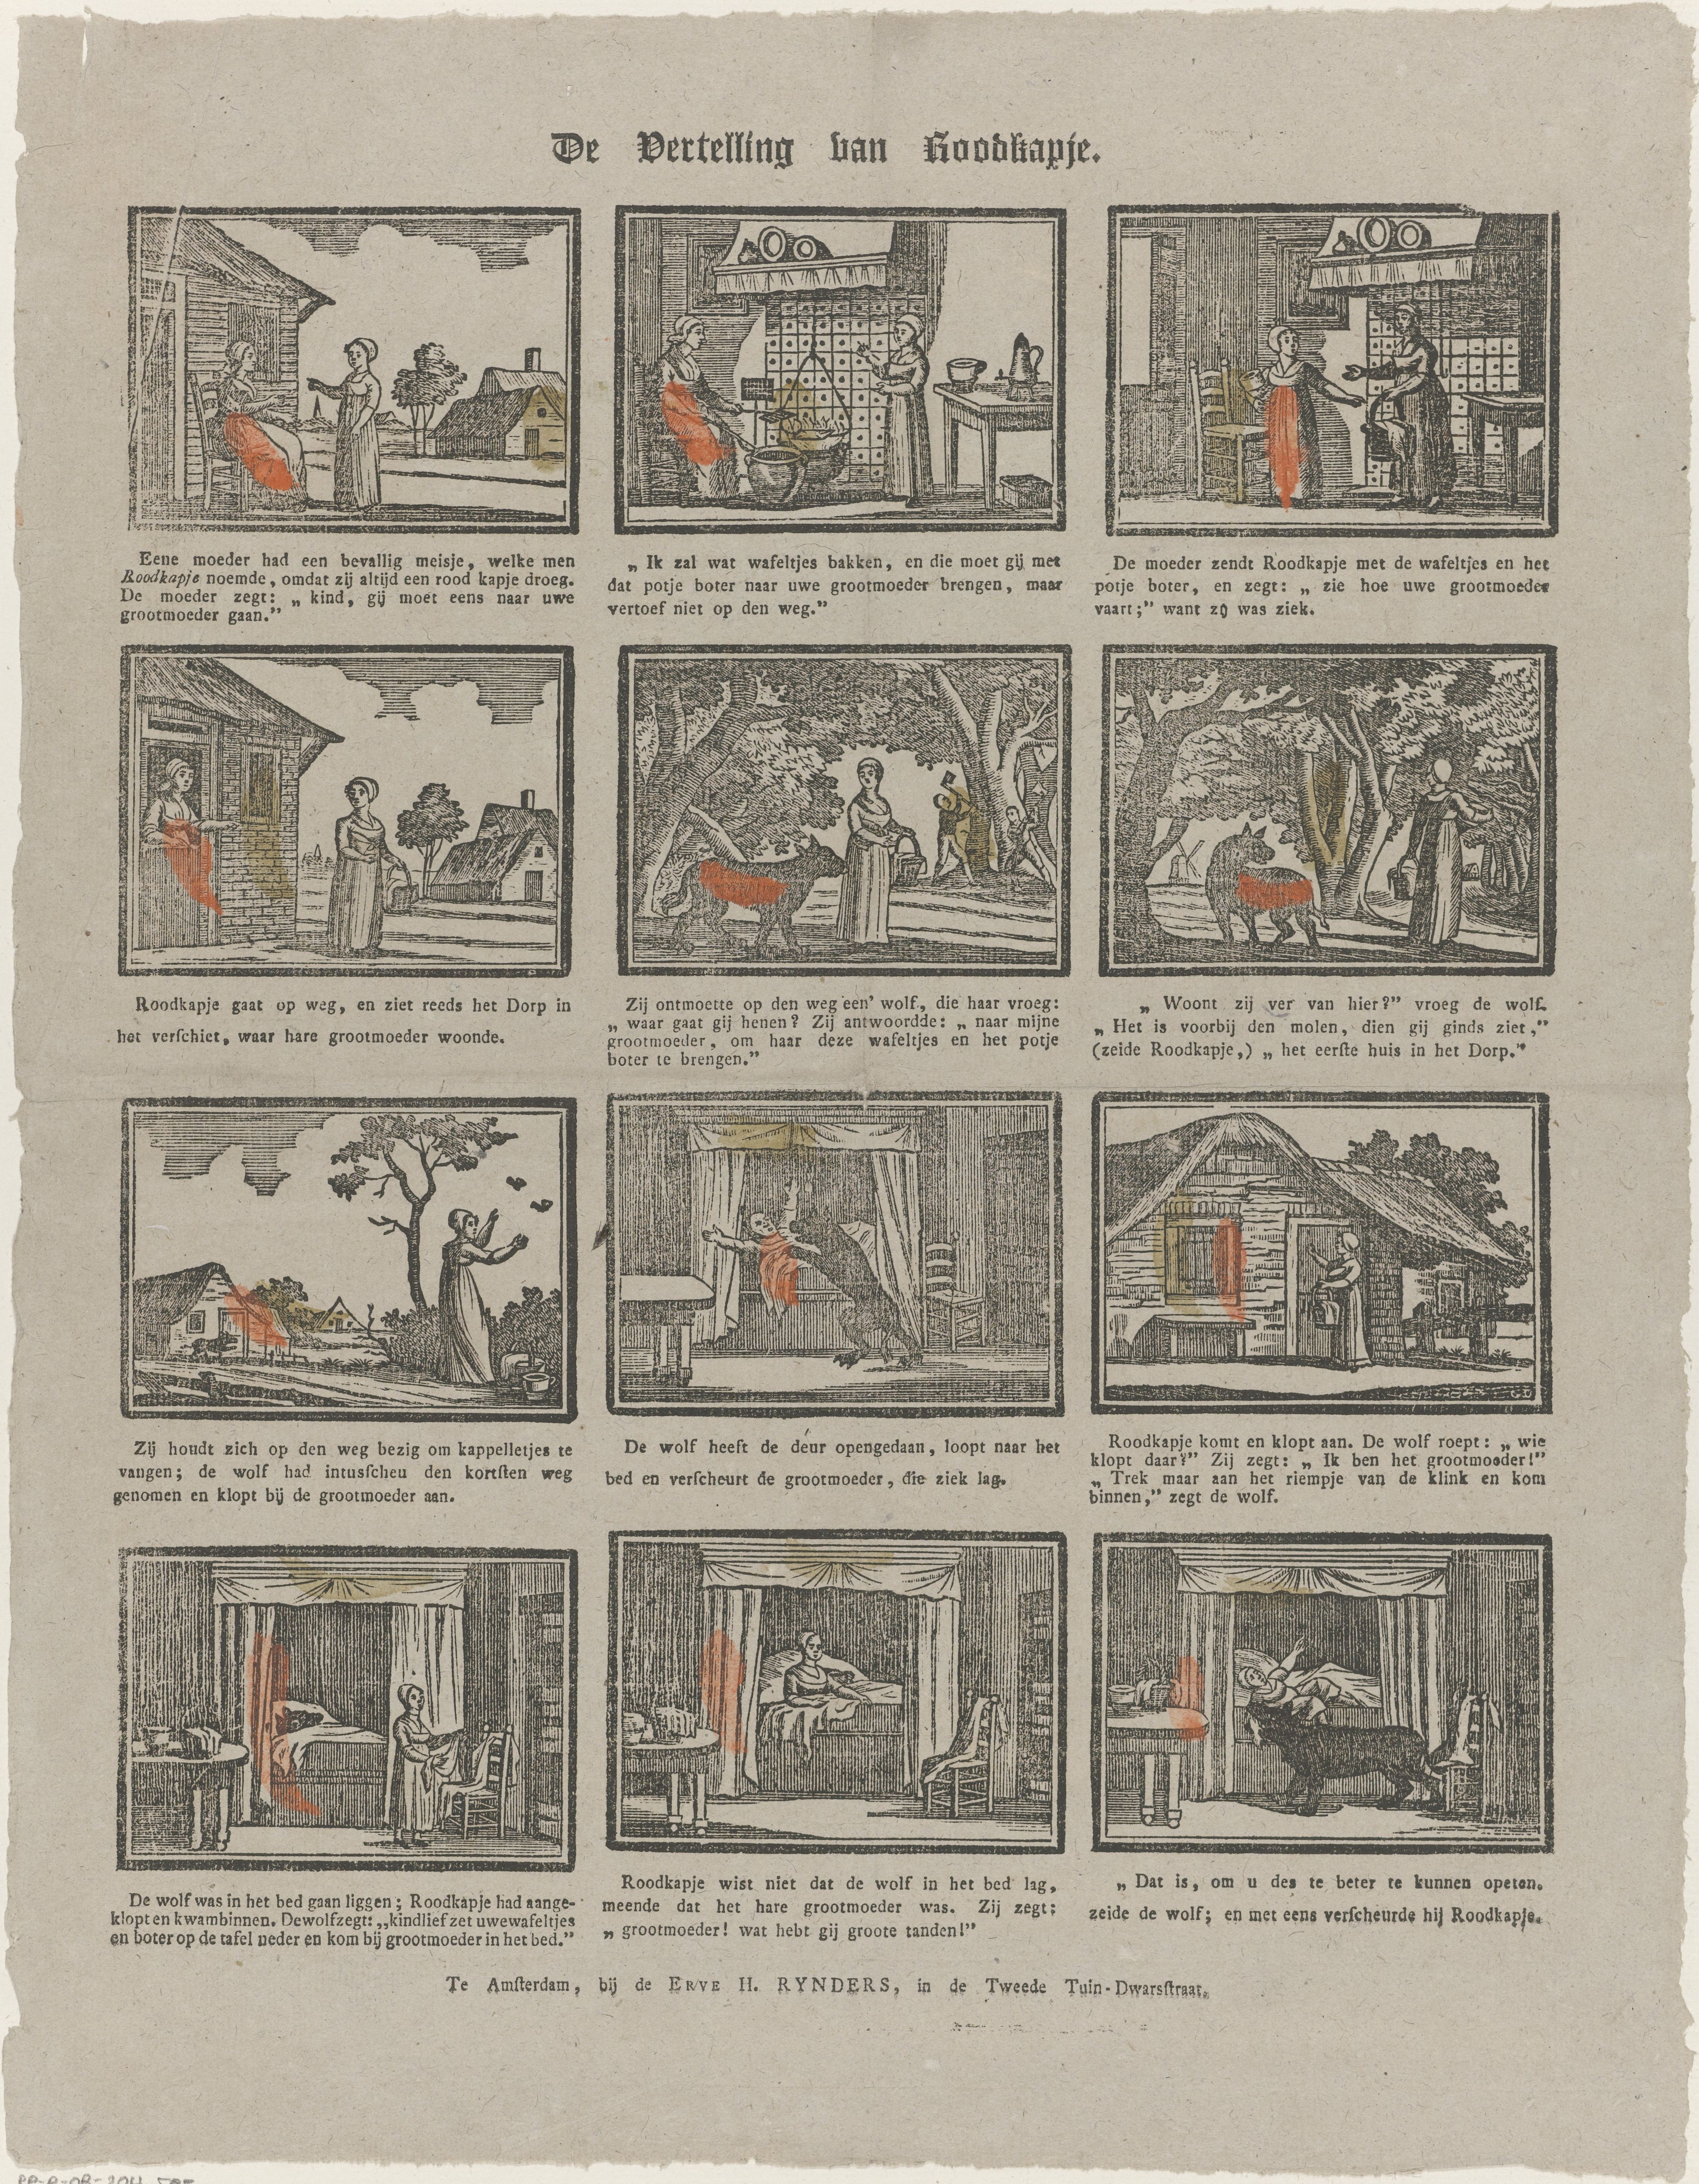
\includegraphics[width=\textwidth]{images/pennycatch}
\caption{\emph{De vertelling van Roodkapje}, Erve H. Rynders, 1831 -- 1854.}
\label{fig:pennycatch}
\end{figure}

The oldest Dutch translation in my corpus of ``Red Riding Hood'' retellings (see section \ref{sec:data}) is entitled \emph{De vertelling van Roodkapje} (`The tale of Little Red Riding Hood') and stems from 1781. This version and most Dutch retellings of ``Red Riding Hood'' in the \nth{19} century adhere to the plot structure of Perrault's story. The suggestive rhyming moral, however, is either set aside or altered by many authors. It is interesting to note that many retellings bear the word \emph{nieuw} (`new') in their title as in the anonymous 1818 version \emph{De Nieuwe Geschiedenis van Roodkapje} (`The new history of Red Riding Hood'). As \citeauthor{beckett:2002} remarks, this reminds us ``that retellings have always been an attempt to rejuvenate the tale for a contemporary audience''\autocite[xvi]{beckett:2002}. Many of the oldest versions of ``Red Riding Hood'' in the Netherlands were published as so-called pennycatch prints. Pennycatch prints were the cheapest illustrated printed material -- for one or a few pennies -- and report on important events or tell popular stories such as ``Red Riding Hood'' on a single sheet of paper, slightly larger than the current A3-format. Figure \ref{fig:pennycatch} provides an example one of the pennycatch prints in the collection. 

\subsection{Grimms' Story of Discipline}
The second classic retelling of ``Red Riding Hood'' is the one by the Brothers Grimm, \emph{Rothkäpchen}, originally published in 1812 in the collection \emph{Kinder- und Hausmärchen}. The most striking change made by the Brothers Grimm is the rescue scene of Little Red Cap by a hunter. Little Red Cap may not be killed, yet it could be argued that the Brothers Grimm emphasize the image of a naive and helpless girl even more\autocite[32]{zipes:1993}. In contrast with the oral versions, Little Red Cap is unable to save herself and is dependent on the protection of a father figure. The Brothers Grimm have reworked and revised their collection several times in an attempt to adapt the story to fit the emerging Biedermeier image of a child: Little Red Cap must show obedience and good behavior\autocite[32--37. For an automatically generated alignment of the seven versions published by the Brothers Grimm, see \texttt{http://fbkarsdorp.github.io/grimms}.]{zipes:1993}. The emphasis on good behavior is apparent from the added cautionary scene in which Little Red Cap is warned about the dangers of talking to strangers, straying from the path or lingering in the woods. In the 1850 and 1857 edition, the Brothers Grimm stress the importance of good manners when the mother commands the girl: ``Und wenn du in ihre Stube kommst, so vergiß nicht guten Morgen zu sagen und guck nicht erst in alle Ecken herum.''\footnote{`And when you enter her parlor, don't forget to say `Good morning', and don't peer into all the corners first.'} Little Red Cap promises to be obedient, but she is not, and therefore she needs to be punished. At the end of the story, Little Red Cap is aware of her disobedience and concludes that she is to be held responsible for her fate. Some Dutch retellers have emphasized this lesson using a more elaborate moral, as in the version by Simon Jacobus Andriessen (1880): ``Die kwaad doet, kwaad ontmoet! en: Wie niet hooren wil, moet voelen!'' (`He that mischief hatches, mischief catches!' and: `He that will not be counseled cannot be helped!'). 

\begin{figure}[t]
    \centering
    \includegraphics[width=\textwidth]{images/battle}
    \caption{Population plot showing the fraction of retellings per decade of ``Red Riding Hood'' classified as a version of either Perrault, the Brothers Grimm, or `other'.}
    \label{fig:battle}
\end{figure}

Perrault's tale and the retelling of the Brothers Grimm have been popular in the Netherlands. However, the number of retellings that showed signs of being influenced by the Brothers Grimm directly after \emph{Kinder- und Hausmärchen} was published in 1857 is rather low. Over the years the numbers gradually increased before it `took off' in the 1890s and ``it virtually dwarfed Perrault's version''\autocite[36]{zipes:1993}. Figure \ref{fig:battle} visualizes the competition between Perrault and the Brothers Grimm from the late \nth{18} century to the early \nth{21} century in the Netherlands. The plot shows for each decade from 1780 to 2010 the fraction of retellings that can be classified as a version derived from either Perrault, the Brothers Grimm or `other'. A retelling is classified as a Perrault version if both the grandmother and the girl are eaten by the wolf and they are not rescued. A version counts as a retelling of the Brothers Grimm if, after being swallowed, both the grandmother and the girl are saved from the wolf's belly. The `other' group shows the fraction of versions in which the grandmother is devoured (without being rescued) while the girl is saved before the wolf is able to lay a hand on her. Without more information about the rest of the narrative, it is hard to say whether these versions adhere to the Perrault or to the Grimm paradigm. They do fit the trend of `Victorian censorship' of the \nth{19} century in which scenes considered to be too cruel or too sexual were replaced. 

\begin{figure}
\centering
\includegraphics[width=\textwidth]{images/anonymous}
\caption{Fraction of anonymous (versus authored) retellings of ``Red Riding Hood'' over the period 1870 -- 1950.}
\label{fig:anonymous}
\end{figure}

It is interesting to observe that the explosive burst of retellings within the Grimm paradigm is followed by a `stabilizing' period at the beginning of the \nth{20} century in which no radical changes to the story are made. As illustrated by Figure \ref{fig:anonymous}, this is also a period in which a large number of anonymous retellings of ``Red Riding Hood'' were published, possibly to evoke an image of authenticity as a tale from oral history. Furthermore, quite a number of retellings position themselves explicitly in relation to either Perrault or the Brothers Grimm. An example from my corpus appeared in the collection \emph{Sprookjes Van Moeder De Gans} (`Fairy tales by Mother Goose') written by Christine Doorman (1916). Although the title of the collection refers to Perrault, the story of ``Red Riding Hood'' more closely resembles the plot structure of the Brothers Grimm with its reassuring rescue scene. The beginning of the \nth{20} century might be epitomized as a period in which the fairy tale becomes increasingly generic and autonomous, not bound to a particular author but residing in the collective imagination. In this context, Soriano aptly suggests that the fairy tale has become a text ``without a text'' and a text ``without an author''\autocite[cited in][xvii]{beckett:2002}.

\subsection{Time for Change}
We might hypothesize that within the context of a literary environment in which there is a strong tradition of the story, yet it is not linked to a specific author, retellers are able to engage more freely with the material\autocite{beckett:2002}. Starting from the 1940s but especially in recent decades, an increasing number of retellings expose radical innovations, aesthetic experimentation and intertextual references. Because of their limited exposure to cultural heritage, children are generally assumed to be less competent in decoding these intertextualities. \citeauthor{beckett:2002} argues that in the case of ``Red Riding Hood'', authors \emph{can} use these sophisticated narrative strategies, because they can safely assume children know at least some version of the story, which provides them with the necessary decoding tools\autocite{beckett:2002}.

\begin{figure}
    \centering
    \includegraphics[width=\textwidth]{images/vendel_wolfdood}
    \caption{\emph{Rood Rood Roodkapje}, by Edward van de Vendel; illustration: Isabelle Vandenabeele (2003).}
    \label{fig:red-red}
\end{figure}

After World War II, the story of ``Red Riding Hood'' branched off in too many directions to enumerate in this overview. \citeauthor{zipes:1993} distinguishes three major branches: (i) retellings in which ``Red Riding Hood'' becomes increasingly independent, (ii) versions that rehabilitate the wolf and/ or tell his version of the story and (iii) stories that stand out with respect to their aesthetic experimentation\autocite[59]{zipes:1993}. I discuss an example from each of these branches to illustrate some of the radical changes the story has undergone.

\subsubsection*{Rood Rood Roodkapje}
The retelling \emph{Rood Rood Roodkapje} (`Red Red Red Riding Hood') by the Dutch author Edward van de Vendel with illustrations by the Flemish illustrator Isabelle Vandenabeele, is an exciting example of a retelling in which Red Riding Hood has become self-reliant\autocite{vendel:2003}. Vandenabeele makes use of a drawing style that is reminiscent of the etchings by Gustave Doré, yet much coarser and only in the colors gray, black and red. Red Red Red Riding Hood only wishes for red things, red clothes, red juice, red carpet, red pillows on her bed. She had to choose her own name -- the reversal of a dominant motif in ``Red Riding Hood'', which is iconic of her more independent status. All her wishes are red, but her days are gray, because she has to walk the gray muddy paths everyday to her gray grandmother. Then one day, she encounters something black\ldots The Wolf. By accident she shows the Wolf the way to her grandmother. The Wolf immediately spurts to her grandmother and devours her with a terrifying howling sound. Determined to make up for her mistake, Red Red Red Riding Hood follows the Wolf to her grandmother's house. No, this time there is no howling 

\begin{quotation}
\noindent
{\fontsize{2cm}{1em}\selectfont%
grwarwah\vspace{0.5cm}\\
briaaauwah\vspace{0.5cm}\\
hgroing\vspace{0.5cm}\\
raaaaaaaaa\vspace{0.5cm}\\}
\noindent {\scriptsize But: chop.}
\end{quotation}

After the restrained slaying scene, we see a calm girl with a somewhat subdued and contemplative look on her face, holding a bloody ax, while the blood flows from her grandmother's doorway (cf.\ Figure \ref{fig:red-red}). Content with the thought that she never has to visit her grandmother again, Red Red Red Riding Hood imagines all the red things she can do in her life. As in the old French oral version of the story in which ``Red Riding Hood'' outwits the wolf, Van den Vendel and Vandenabeele present a girl who is no longer timid, innocent or powerless, but rather fearless, determined and self-assured.

\begin{figure}[t]
    \centering
    \includegraphics[width=\textwidth]{images/Waterwolf}
    \caption{\emph{De Wolf die tegen water praatte}, by Imme Dros; illustration: Henricus Geelen (1991).}
    \label{fig:waterwolf}
\end{figure}

\subsubsection*{De Wolf die tegen water praatte}
At an abstract level, the story \emph{De Wolf die tegen water praatte} (`The Wolf who talked to water') by the Dutch author Imme Dros, closely resembles traditional retellings of ``Red Riding Hood'': (i) A girl meets a wolf in the forest, (ii) the wolf swallows both the girl and her grandmother, (iii) they are rescued by a hunter, and (iv) the wolf, filled with stones, drowns in the water\autocite{dros:1991}. The perspective of the story, the ordering of the different plot elements and especially the meaning attributed to these elements, however, is completely different. The story, reminiscent of Ovid's \emph{Narcissus}, tells us about the wolf Noordenloos (`Northless') whose only friend is his reflection in the water (cf.\ Figure \ref{fig:waterwolf}). The lonely Noordenloos wishes to return to his former wolf pack in the North together with his imaginary friend Waterwolf. One day, after having a conversation with Waterwolf, Noordenloos meets a girl, who asks for directions to her grandmother's cottage. Following the traditional plot structure, the wolf arrives at grandmother's house before Red Riding Hood does, swallows the grandmother, tricks Red Riding Hood using his famous disguise, and finally, gobbles her up. However, unlike in most traditional retellings, the primary reason for eating Red Riding Hood and her grandmother is not to stave off hunger, but serves to strengthen the wolf for his escape from loneliness to the North. Yet, he only manages to join his family in the North in his own imagination at the moment of his -- metaphorically described -- death: he was happy. By approaching the story from the wolf's perspective, Dros transforms the wolf from being primarily `Big and Bad' into a real character with a soul, feelings, thoughts and desires. 

\subsubsection*{Roodkapje en de zeven geitjes}

The experimental retelling written by Ivo de Wijs with illustrations by Alfons van Heusden (\citeyear{wijs:1994}) diverges radically from the tradition, both in form and in content. The story is part of a collection entitled \emph{Roodkapje en de zeven geitjes} (`Red Riding Hood and the Seven Kids'). This rather unusual juxtaposition of characters from two famous fairy tales serves to emphasize the bricolage nature of the stories to come. Each story in the book tells three different versions of a story. On each page, supposedly aligned fragments of the three versions are placed side by side in three columns, each with its own distinctive typography. The reader is supposed to read all three columns before moving on to the next page (see Figure \ref{fig:dewijs} for a translation of the first paragraphs of each version).

\begin{figure}
{
\centering
\begin{tabular}{>{\raggedright}p{0.3\textwidth} >{\raggedright}p{0.3\textwidth} >{\raggedright\arraybackslash}p{0.3\textwidth}}
{\oldstyle Once upon a time there was a little girl who lived with her mother in a small house near the forest. Everyone called the girl Little Red Cap, because she wore a red cap, which her grandmother gave to her. One day her mother said to her: `Child, your grandmother fell ill. Go pay her a visit. Here is a basket with wine and biscuits. But remember: don't tarry on your way and don't stray from the path in the forest. I hope that grandmother will soon feel better!'}

&

{\intstyle On the edge of the forest lived a little girl in a small house. Everyone called her Little Red Cap because her house had a red roof. One day her father said to her: `My dear child, it's your grandmother's birthday. Here is a basket with presents for her: a bottle of wine, a can of biscuits and a bouquet of flowers. Go bring the basket to her, but remember: don't loiter on your way! Say my regards to grandmother and wish her congratulations! And many years to come!'}

&

{\newstyle Once upon a time there was a little girl called Gretel. Well, her name was Gretel, but she was called Little Red Cap because of her flaming red hair. Little Red Cap lived with her grandmother in an old tower out in the woods. One day grandmother went to the city to buy biscuits and lemonade -- and a cough medicine because Little Red Cap wasn't feeling well. `Come back soon, grandmother,' said Little Red Cap, `walk briskly!' And grandmother went on her way.}
\end{tabular}
}
\caption{First paragraphs of \emph{Roodkapje} by Ivo de Wijs \citeyearpar{wijs:1994}, translation FK.}
\label{fig:dewijs}
\end{figure}

The first column of \emph{Roodkapje} closely resembles a `traditional' version of ``Red Riding Hood''. The second version adheres to the traditional plot, yet it adapts and reworks many well-known motifs. The origin of Little Red Cap's name, for example, stems from the red roof of her house. Here De Wijs makes playful use of the fact that the noun \emph{kap} in the compound \emph{Roodkapje} can refer to both a cap and a roof in Dutch. Another small change in the opening scene is that Little Red Cap's father (and not her mother) sends her to her grandmother. Furthermore, the purpose of her trip is to visit her grandmother because of grandmother's birthday and not because granny has fallen ill. In the forest, Little Red Cap meets the wolf, who is rather fond of the biscuits the girl brought with her. He is not allowed to have any and therefore decides to take a piece of the grandmother. When the wolf arrives at the doorstep of grandmother's house, grandmother distrusts the visitor because of his low voice. Using a piece of chalk to raise his voice -- a motif borrowed from \emph{The Wolf and the Seven Kids} -- the wolf finally manages to convince the grandmother to let him in. The traditional formulaic scene has undergone some changes as well. This time Little Red Cap does not marvel about grandmother's physiognomy, but about about the size of her nightcap and her big glasses. The traditional savior of Little Red Cap and her grandmother is replaced by a butcher. After being rescued from the wolf's belly, the butcher, Little Red Cap and the grandmother hide in the clock -- again an allusion to \emph{The Wolf and the Seven Kids} -- in anticipation of what will happen next. In the climactic scene of the story, the wolf, in search of food, sticks his head into the oven. In this scene, Little Red Cap assumes the role of Gretel from \emph{Hans and Gretel} as she pushes the wolf into the oven.

The third version of the story is truly disorienting. The story is replete with references to other stories, blendings of motifs, reversals of situations, and replacements of characters. In her discussion of the story \citeauthor{beckett:2002} described Little Red Cap's identity in this third variant as one ``in a constant state of flux''\autocite[100]{beckett:2002}. Just as in the second version, yet more overtly, Little Red Cap assumes the roles of various female fairy tale characters. This role-shifting already starts in the introductory scene, in which it explained that because of her red flaming hair, everyone calls the girl Little Red Cap, but her actual name is Gretel. She lives with her grandmother out in the woods in a tower, which immediately brings the story of Rapunzel to mind. The grandmother and Little Red Cap change roles. It is the grandmother who goes into town to buy biscuits, lemonade and a cough medicine for her sick granddaughter, and it is the grandmother who encounters the wolf in the forest. After revealing to the wolf where she is going, the wolf spurts to Little Red Cap's tower -- at which moment the reader finds out that the tower is actually the property of Snow White. Unable to find an entrance, the wolf waits for the grandmother to come home to find out how to enter the tower. When the grandmother arrives at the tower, she assumes the role of the witch in \emph{Rapunzel}, claps her hands and commands Little Red Cap to let down her braids. After devouring granny, the wolf climbs up the braids. Little Red Cap is scared by the hairy look of the wolf, but it is not Little Red Cap who is gobbled up, but Rapunzel. The wolf disguises himself as Sinterklaas (wearing a bishop miter) and goes to bed. The savior of the story is a young prince, called Hansel, who, after transforming himself into a raven, flies to the tower. There he assumes his normal form, cuts open the belly of the wolf and saves Cinderella and her grandmother. The dead wolf is thrown out of the window, and by using another magic spell, the prince transforms the grandmother, Sleeping Beauty(!) and himself into ravens, which enables them to escape from the tower. Once they are transformed back into their normal forms, the grandmother and Gretel follow the prince to his homeland. The prince and grandmother get married and they live happily ever after.

The three retellings by De Wijs describe a micro-level development that reflects the development of ``Red Riding Hood'' on a macro-level. The stories form each other's pre-text, they echo each other -- to use the words of \citet[37]{frank:2010}. Reading De Wijs' retellings can be considered as an individual experience of a process of gradual accumulation of modifications, the same process I hypothesize to be the driving force behind the development of ``Red Riding Hood'' at the population level. Before I will present the methods to investigate this hypothesis, I will first provide a detailed overview of the data collection used in this study.

\section{Data Collection and Data Annotations}

\subsection{Data Collection}\label{sec:data}
The Koninklijke Bibliotheek (National Library) of the Netherlands is in possession of a tremendously rich collection of children's books. It consists of over 195 thousand books that have been collected over a period of two hundred years. The collection contains about 630 versions of ``Red Riding Hood'', of which the oldest version dates from the late \nth{18} century and the latest from 2015. Many versions are part of the Special Collections department of the National Library, which contains books and manuscripts that are too old, rare, precious or fragile to be made available through general circulation. For this study, I required a full-text version of the collection, yet only a handful of retellings of ``Red Riding Hoods'' have been made digitally available. To remedy this problem, I digitized all available versions listed in the catalog of the National Library (with the exception of reprints). The stories were either manually transcribed or by means of OCR followed by manual post-correction. After removing duplicates, the total number of stories in the digitized version of the collection amounts to 440\autocite[][See \texttt{http://fbkarsdorp.github.io/rrh-browser} for a bibliography of all stories as well as an interactive search engine of the collection.]{folgert_karsdorp_2016_51588}. The meta data for each story include: the title, author, (optional) collaborator, (optional) illustrator, (estimate of) year of publication, publisher and the dimensions of the book.

\begin{figure}
\includegraphics[width=\textwidth]{images/statistics}
\caption{Diachronic visualization of some general statistics about the ``Red Riding Hood'' corpus. The subplots (from left to right) in this figure visualize: the average $z$-scores of the document length per year (expressed in word forms), the average $z$-scores of the sentence length per year (expressed in word forms) and a kernel density plot of the year of publication of the stories.}
\label{fig:corpus-statistics}
\end{figure}

I constructed a tokenized version of the ``Red Riding Hood'' collection using the tokenizer Ucto.\footnote{See \url{https://languagemachines.github.io/ucto/} and corresponding manual \url{https://github.com/LanguageMachines/ucto/raw/master/docs/ucto_manual.pdf}.} The total number of words in the tokenized version amounts to 493,169 (including punctuation). In their lowercased form, 10,683 of these word forms occur uniquely. On average each year in the corpus ranging from 1781 to 2015 is represented by about 3 stories. Stories consist of 1155 word forms on average. Some of the general statistics of the corpus have been diachronically visualized in Figure \ref{fig:corpus-statistics}. The subplots (in order of appearance) in this figure visualize the average document length per year, the average sentence length per year and the number of retellings of ``Red Riding Hood'' published in a particular year. For reasons of comparability, I normalized the frequencies in the first two plots to their $z$-score. As can be observed from the density plot over the publication years of the stories, the corpus is rather skewed towards more recently published versions of ``Red Riding Hood''. This bias will be taken into account in the subsequent analyses. Looking at the first subplot, we can observe that the document length of the stories remains generally stable over time. When we inspect at the average sentence length, however, we note a steady decrease starting at the beginning of the \nth{20} century. We might hypothesize that this trend fits a development in which authors more and more adapt their retelling towards their young readers, who generally prefer shorter over longer sentences. However, more materials and research are required to assess whether the observed trend is representative of a development in children's literature at large. 

\subsection{Story Annotations}\label{sec:annotations}

Variation is one of the three preconditions described by Darwin for biological evolution. Without variation, there is nothing to be selected and hence no change can take place. Because of its central position to his theory, Darwin documents the variation he observed between members of the same species in great detail. An exemplary quote about variation about pigeons reads as follows:
\begin{quote}
    The proportional width of the gape of mouth, the proportional length of the eyelids, of the orifice of the nostrils, of the tongue (not always in strict correlation with the length of beak), the size of the crop and of the upper part of the oesophagus; the development and abortion of the oil-gland; the number of the primary wing and caudal feathers; the relative length of wing and tail to each other and to the body; the relative length of leg and of the feet; the number of scutellae on the toes, the development of skin between the toes, are all points of structure which are variable.\autocite[Darwin \emph{The Origin of Species}, cited in][27]{mesoudi:2011}
\end{quote}
\citeauthor{mesoudi:2011} argues that to justify the description of cultural change as a Darwinian evolutionary process, we must show that culture exhibits the same preconditions as biology\autocite[27--34]{mesoudi:2011}. An adaptation of Darwin's description of pigeon variation to ``Red Riding Hood'' could read as follows:
\begin{quote}
    The fabrics of Red Riding Hood's cap (cotton, silk, wool), the contents of her basket (is she carrying wine, bread, waffles, butter, juice, cake, lard), whether or not the girl meets with the wolf in the woods, the surroundings of grandmother's cottage (oaks, a hedge, a mill), whether the wolf eats granny and or Red Riding Hood and in what way (swallowing, gobbling, devouring, guzzling), whether the girl and her grandmother are saved and by whom (a woodcutter, a hunter, her father, animals in the forest), whether the wolf is killed and in what way (using an ax, a gunshot, a bat), whether the wolf's belly is filled with stones and who puts the stones in his belly, are all points of the story which are variable.
\end{quote}
Like Darwin, I could go on like this for several pages. If we look closely at all the different retellings of the story, the amount of variation is truly overwhelming. To establish a mapping of the variation, I subjected all 440 stories in the corpus to a questionnaire of more than 300 questions. The questionnaire consists of simple ``yes-no'' questions (e.g.\ \emph{Does the story explain the origin of Red Riding Hood's name?}), multiple choice questions (e.g.\ \emph{Where does Red Riding Hood encounter the wolf? (a) on the path, (b) away from the path, (c) somewhere else, (d) they don't meet}) and open questions (e.g.\ \emph{What is the lemma of the verb used to describe the wolf's eating of Red Riding Hood?}). Most questions in the questionnaire fit concepts from structural text analysis and narratology\autocite[E.g.][]{bal:2009,vanboven:2003}. The list of potential questions is virtually endless. I have attempted to compile a list of questions of which the answers constitute a detailed and rigorous text analysis. The questions can be classified under the following six categories: (i) genre, (ii) narration, (iii) space, (iv) motif, (v) time and (vi) character. 

\begin{figure}
    \centering
    \includegraphics[width=\textwidth]{images/genre}
    \caption{Population plot of the five most frequently occurring genres in the ``Red Riding Hood'' collection. We calculate the fraction of stories published in a particular genre for every 50 years.}
    \label{fig:genre}
\end{figure}

\paragraph{(i) Genre} In the category `genre' we find questions designed to distinguish between kinds of stories in form and content. The collection of ``Red Riding Hood'' retellings contains the following genres: regular stories, picture books, pop-up books, theater, comics, puzzles, picture story, catchpenny prints and poems. A story with illustrations is not necessarily classified as a picture book. Only stories in which the pictures take central position with an accompanying text are considered to be picture books. As some stories belong to multiple genres, it was allowed to provide multiple answers. As can be observed from Figure \ref{fig:genre}, poems were a popular form for Dutch authors to tell the story in the second half of the \nth{19} century, whereas in more recent years, we discover a steady increase in the number of picture books. 

\paragraph{Narration (ii)} The second category of questions deals with the narration of the story. Most importantly, this category addresses the narrator of the story or -- in narratological terms -- the question of the speech-position from which the narrative contents of a story as a whole originates. Most versions of ``Red Riding Hood'' are classified as third-person narratives. In recent years retellers of ``Red Riding Hood'' have experimented with different forms of narration such as the first-person narrative. An interesting example of a first-person retelling is the one by the Dutch author Ivo de Wijs, which is part of the collection \emph{En ze leefden nog\ldots Sprookjes op Rijm}\autocite{wijs:2011}. The potentially hilarious effect of telling ``Red Riding Hood'' from a first person point of view becomes especially clear after Red Riding Hood is gobbled up by the wolf:

\vspace{\abovedisplayskip}
\begin{minipage}[c]{\textwidth}
\begin{Parallel}[c]{0.5\textwidth}{0.5\textwidth}
{\small
\ParallelLText{
\noindent
In de maag van het gulzige beest\\
Zat mijn oma, een tikkie bevreesd\\
Ze zei: `Meisje, je komt als geroepen\\
Want we moeten hier dadelijk uit\\
Stel je voor dat dat monster besluit\\
Ons gezamenlijk uit te gaan poepen'
}

\ParallelRText{
\noindent
In the tum of the devouring beast\\
Was my granny, a little afraid\\
She said: `Girl, you're just in time\\
Because we have to leave immediately\\
What if that the monster descides\\
to poop us out collectively'
}
}
\end{Parallel}
\end{minipage}

\vspace{\belowdisplayskip}
\paragraph{Space (iii)} The third category of questions deals with space. The questions aim to collect information about e.g.\ the location or the surroundings of grandmothers house. 

\paragraph{Motif (iv)} The largest group in the questionnaire is category four, which contains various questions about smaller and larger motifs, e.g.\ \emph{Is Red Riding Hood eaten by the wolf?}\ or \emph{Is the wolf's belly filled with stones or some other material?}. Category four also queries the main episodes of the story. Examples of questions are: \emph{Does the story contain a cautionary scene in which the mother of Red Riding Hood warns her about the dangers in the forest?} and \emph{Does the text describe a scene in which Red Riding Hood returns back home?} The Grimms' version of ``Red Riding Hood'' contains a rarely retold and virtually unknown second ending to the story. In this ending -- a kind of epilogue or sequel -- Red Riding Hood, barely recovered from her previous adventures, visits her grandmother again. In the woods she meets another wolf but this time she shows obedience and proves that she has learned her lesson. Together with her grandmother she manages to kill the wolf by making him fall from the roof into a big stone trough. The Dutch ``Red Riding Hood'' collection contains thirteen version in which this second episode is retold.

\paragraph{Time (v)} The category `time' contains questions that discuss the ordering of events, the passing of time and tension and irony. Examples of questions are: \emph{Does Red Riding Hood encounter the wolf before or after she strays from the path?} and \emph{If the wolf is killed, does that happen before or after Red Riding Hood (and her grandmother) are rescued?}. Questions about irony and tension were included in the category time, because they deal with expectations and anticipations of readers (e.g.\ `What will happen next?'). The climactic scene of the wolf in disguise can be read as an example of dramatic irony in which the girl naively believes the wolf to be her granny. To be able to understand this irony, children must have grown a `theory of mind', which allows them to reason about others in terms of goals and intentions. Theory of mind is one of the most important concepts in social-psychology and social evolution theory\autocite[see e.g.][]{tomasello:1999}, yet literary and folktale studies have only scantily paid attention to it\autocite[Cf.][]{boyd:2009}. In the development of a full-blown theory of mind, children learn about `beliefs' and `false beliefs'. In the context of ``Red Riding Hood'', this knowledge enables children to understand that the girl \emph{believes} that it is her grandmother lying in the bed, yet they know about the actual state of things and hence that this belief is false. Knowledge about (false) beliefs is of crucial importance in our life to make predictions about the behavior and intentions of others. ``No wonder,'' \citeauthor{boyd:2009} argues, ``that point of view and dramatic irony play such central roles in fiction, or that the gap between appearance and reality is such a wide-spread theme''\autocite[149]{boyd:2009}. Retellings of ``Red Riding Hood'' play with this theme. Sometimes authors explicitly anticipate the potential downer ending at the outset of the story, especially when there is no salvation scene. In other retellings, authors feel the need to make explicit that after being swallowed, the girl and her grandmother are still alive and well in the tummy of the wolf. Yet other versions omit the traditional switch of perspective from Red Riding Hood to the wolf and continue to keep track of the actions of the girl. In such versions, it is not yet clear to the reader who lies in the bed at the moment the girl arrives at her grandmother's cottage. This narrative strategy leads to a reading of the story without false belief and has a stronger effect of surprise. 

\paragraph{Character (vi)} Without the characters there would be no story. The last category contains questions about the participants in the stories. These include questions about the presence or absence of characters (e.g.\ \emph{Is Red Riding Hood's mother present in the story?}), about their physical properties (e.g.\ \emph{Does the story describe any physical properties of Red Riding Hood?}), about their clothing (e.g.\ \emph{Does the text make explicit reference to Red Riding Hood's hood?}), or about their personality traits (e.g.\ \emph{Is the wolf referred to as a ``(big) bad wolf''?}). 

\subsection{The Rise of the Big Bad Wolf}
In this section, I highlight one group of questions in some detail, viz.\ those dealing with the way characters are introduced to the story. Writers and storytellers have two basic introduction strategies to their disposal: They can introduce a character by means of (i) \emph{indefinite} reference (using an indefinite article, e.g.\ Dutch \emph{een}) or (ii) \emph{definite} reference (using a proper name or a definite article, e.g.\ Dutch \emph{de}).\autocite[See e.g.][]{deJong:1987,lyons:1999,radden:2007} Indefinite reference is generally used to introduce `new information', i.e.\ information the writer deems inaccessible to the reader. Definite reference, on the other hand, is typically used to refer to `given information' in which case the writer assumes that the reader is able to identify the intended referent. Folktale characters are typically introduced as `new' -- hence, their referent is introduced by means of an indefinite article at first mention, as in the following opening sentence from Perrault's \emph{Le petit Chaperon rouge}: ``Once upon a time there was \emph{a} little village girl\ldots'' Once introduced, the girl becomes given information, i.e.\ she becomes part of the set of referents that can be assumed to be accessible to the reader. This allows the writer to refer to the girl using definite reference in subsequent parts of the story. In the linguistic literature, the concept `discourse reference' is employed to indicate this transition from indefinite to definite reference, as it depends on the progression of discourse\autocite[98]{radden:2007}. Referents can also count as given information when they are (assumed to be) part of the shared socio-cultural world knowledge of a writer and a reader. This type of reference is called `unique reference'\autocite[99]{radden:2007}. Such entities can be referred to by means of definite reference even though they have not been introduced in the preceding discourse. 

I hypothesize that with the increasing familiarity of the story over time and its consequent entrenchment in culture\autocite[Cf.][]{beckett:2002}, the characters of ``Red Riding Hood'' become more and more part of the shared world knowledge of a writer and her or his audience. In other words, they become `given information'. Readers have expectations about the course of the story and appearance of certain characters, and writers assume their audience to know at least some version of the story. Indicative of their expectations, readers often act surprised when they discover that there is no rescuer in Perrault's version of the story. The entrenchment of the characters is exemplified by what \citeauthor{beckett:2002} calls fairy tale salads\autocite[Cf.\ chapter 7 in][]{beckett:2002}. These are stories in which characters from various popular fairy tales are transferred to new contexts without loosing their identity and accompanying literary and cultural expectations.

\begin{figure}
\centering
\includegraphics[width=\textwidth]{images/definite}
\caption{Plots showing definite (points with a value of 1.0) and indefinite references (points with a value of 0.0) used to introduce the wolf and Red Riding Hood in the corpus. The line represents the regression model fits to these points, the shade of which shows the confidence intervals.}
\label{fig:definite}
\end{figure}

If my hypothesis holds, we may expect an increase over time in the use of unique reference to introduce the characters of ``Red Riding Hood'' in favor of discourse reference. More specifically, I predict that the probability of introducing the characters by means of definite reference increases as a function of time. In the following analysis, I limit myself to the introduction of the two main characters: Red Riding Hood and the wolf. The question in the questionnaire corresponding to their introduction reads as follows: 
\begin{quotation}
\noindent\emph{Is Red Riding Hood / the wolf introduced to the story by means of definite or indefinite reference?} 
\end{quotation}
To test for the correlation between time and the increased use of unique reference, I subjected the answers given to these questions to two logistic regression analyses (i.e.\ one for Red Riding Hood and one for the wolf). The dependent variable in the regression is whether or not definite reference is used, and the predictor variable is the year of publication of a story. Figure \ref{fig:definite} displays the occurrences of definite and indefinite introductions for the wolf and Red Riding Hood. Points taking the value 1.0 represent introductions by means of definite reference; introductions with indefinite reference take the value 0.0. The curved line represents the fit of the regression model to the data. The shade reflects the confidence intervals of the fit. We can observe that the estimated probability for definite introductions of the wolf increases steadily over time. Analysis of the logistic regression model revealed that the effect of time is significant ($\beta=0.006, \textrm{SE} = 0.002, z = 2.887, p < 0.004$). For Red Riding Hood, by contrast, the plot shows a slight decrease in the estimated probability of definite introductions over time. This effect, however, is not significant ($\beta=-0.003, \textrm{SE}=0.002, z=-1.238, p > 0.2$).\footnote{The time laps in the collection might introduce a bias into the models. To account for this bias, I performed a logistic regression analysis in which the predictor variable `year' is replaced by a variable that increases by 1 with every subsequent year of publication in the corpus. The results of these analyses were similar to the previous ones, both for the wolf ($\beta=0.008, \textrm{SE} = 0.003, z = 2.634, p < 0.008$) and for Red Riding Hood ($\beta=-0.004, \textrm{SE} = 0.004, z = -1.132, p > 0.2$).}

How should we interpret the difference between the two model fits? I suggest that the probability of definite introductions of Red Riding Hood is generally low, because her introduction is constrained by the genre-specific opening sentences in which she is introduced (e.g.\ ``Once upon a time\ldots'' or ``In a country far, far away\ldots''). Because of their conventional nature, such opening phrases request the use of indefinite reference to introduce characters to a story\autocite[For a more general account of opening formulas in folktales, cf.][]{Karsdorp:2013tk}. Interestingly, in the ``Red Riding Hood'' collection these formulaic opening phrases have become even more conventional over time\footnote{The analysis of a logistic regression model shows a significant effect of time ($\beta=0.008, \textrm{SE} = 0.002, z = 3.733, p < 0.000$).}, thus making definite introductions even less likely. The wolf, on the other hand, is predominantly introduced after the cautionary scene, at which moment the constraints of conventional opening phrases no longer apply. The significant increase over time in the use of unique reference to introduce the wolf reflects the increasing familiarity of the story and the consequent expectations of readers about the appearance of certain characters. 

\subsection{Annotation Evaluation}
All stories in the collection have been subjected to the questionnaire. Using a self-developed annotation application\footnote{See \url{http://github.com/fbkarsdorp/roodkapje}.}, I annotated the complete collection. To assess the reliability of the annotations, a second annotator filled in the questionnaire for ten percent of the collection, after which discrepancies with my own annotations were discussed. The amount of agreement between the annotators was measured by means of the $F1$-score.\footnote{Cohen's $\kappa$-statistic \citeyear{cohen:1960} is not suitable for this evaluation, because it is impossible to compute the number of true negatives for certain open questions in the questionnaire.} The results showed strong agreement between the annotations ($F1 = 0.95$). All categorical variables (resulting from multiple choice and open questions) where converted into binary indicator variables. The resulting $m \times n$ matrix $S$ consisted of $m=440$ stories, each of which was represented by $n=2444$ binary variables.

\section{Methods}\label{sec:methods}

\subsection{Distance Measures}
Recall from the introduction that the goal is to identify a set of potential pre-texts for each story in the ``Red Riding Hood'' collection. In this study, I make the simplifying assumption that stories that are more similar to a particular story in terms of their annotations are more likely to have formed their pre-text than other stories. The distance (or similarity) between two stories can be assessed by means of a distance measure, which summarizes the distance between two stories in terms of a pairwise comparison of the answers given to each of the questions in the questionnaire. Importantly, the choice for a particular distance measure can have a severe impact on what is considered to be similar and what is not\autocite[Numerous papers have been published in which various binary distance metrics and similarity coefficients have been proposed. For an in-depth comparison, cf.][]{choi:2010}. 

We can distinguish two main groups of binary distance measures: `negative match \emph{inclusive}' and `negative match \emph{exclusive}' measures. Negative match inclusive measures assume that the absence of two features contributes to the similarity between two objects. In the context of story annotations, this implies that the absence of, for example, the rescue scene in two particular stories adds to the similarity between them. Negative match exclusive measures do not include negative matches in their similarity estimation, and thus do not account for the absence of the rescue scene. The potential downside of negative match inclusive measures becomes especially clear in the context of low frequency features. Take the contents of Red Riding Hood's basket as an example. In only three versions in the collection, Red Riding Hood brings a bottle of milk to her grandmother. Negative match inclusive measures reinforce the similarities between all stories in which the milk is \emph{absent}. Negative match exclusive measures, by contrast, will only reward the similarities between these three versions. More generally, the chance that two stories invoke a negative answer increases as questions become more specific. This does not, however, necessarily imply that the two stories are more similar. 

\begin{figure}
\centering
\includegraphics[width=\textwidth]{images/mismatches}
\caption{Plot showing the differences between the Manhattan distance, Jaccard dissimilarity index and Cosine distance for pairs of vectors with an increasing number of positive matches while keeping the number of mismatches constant at 1. The size of the vectors is 10.}
\label{fig:mismatches}
\end{figure}

In the subsequent analyses, I will compare three binary distance measures: (i) Manhattan distance, (ii) Jaccard dissimilarity index, and (iii) Cosine distance. All three measures have their own assumptions about what is to be considered similar or distant. In what follows, I provide a detailed description of these measures, with which I hope to clarify some of these assumptions.\footnote{For this description I adopt the terminology used by \autocite{choi:2010}.} Let $a$ represent the number of questions to which two stories $i$ and $j$ provide a positive answer. Let $b$ be the number of questions that are positively answered by story $i$ and negatively by story $j$. Finally, let $c$ represent the number of questions negatively answered by story $i$ and positively by story $j$. The sum of $b$ and $c$ represents the total number of mismatches between two stories and is equivalent to the Manhattan distance (also known as the city block distance or $\ell_1$ norm):
\begin{equation}
d_1 = b + c
\end{equation}
The Manhattan distance is an example of a negative match inclusive measure and is based on the assumption that only mismatches contribute to the distance between two stories, and conversely that positive matches and negative matches add to their similarity. 

The Jaccard similarity index is an example of a negative match exclusive measure. It is computed as the number of positive matches ($a$) divided by the sum of positive matches and mismatches ($a + b + c$). In set based terms, it computes the fraction of the length of the intersection between two stories over the size of their union. The complement of this fraction represents the dissimilarity between two stories:
\begin{equation}
d_J = 1 - \frac{a}{a + b + c}
\end{equation}
The Cosine distance is an example of a negative match exclusive measure as well. It is computed as follows:
\begin{equation}
d_C = 1 - \frac{a}{\sqrt{(a + b) \times (a + c)}}
\end{equation}
To get an impression of the effect of each of these distance measures, consider the following four binary vectors, each representing one story: 
\begin{align*}
\mathbf{a}^{(1)} & = \begin{bmatrix*} \dnum{0} & \dnum{1} & \dnum{0} & \dnum{1} & \dnum{0} & \dnum{0} \end{bmatrix*} \\
\mathbf{a}^{(2)} & = \begin{bmatrix*} \dnum{0} & \dnum{1} & \dnum{0} & \dnum{1} & \dnum{0} & \dnum{1} \end{bmatrix*} \\
\mathbf{a}^{(3)} & = \begin{bmatrix*} \dnum{1} & \dnum{1} & \dnum{1} & \dnum{1} & \dnum{1} & \dnum{1} \end{bmatrix*} \\
\mathbf{a}^{(4)} & = \begin{bmatrix*} \dnum{1} & \dnum{0} & \dnum{1} & \dnum{1} & \dnum{1} & \dnum{1} \end{bmatrix*}
\end{align*}
The Manhattan distance $d_1(\mathbf{a}^{(1)}, \mathbf{a}^{(2)}) = d_1(\mathbf{a}^{(3)}, \mathbf{a}^{(4)}) = 1$, because the two pairs contain an equal number of mismatches. The Jaccard dissimilarity index does not consider the negative matches and thus returns a distance of approximately 0.33 between $\mathbf{a}^{(1)}$ and $\mathbf{a}^{(2)}$ and 0.16 between $\mathbf{a}^{(3)}$ and $\mathbf{a}^{(4)}$. As expected, the Cosine distance between $\mathbf{a}^{(1)}$ and $\mathbf{a}^{(2)}$ (0.18) is also larger than between $\mathbf{a}^{(3)}$ and $\mathbf{a}^{(4)}$ (0.08). The magnitude of the difference, however, is larger for the Jaccard dissimilarity index than for the Cosine distance. This effect can also be observed from Figure \ref{fig:mismatches}, which shows the differences between the three distance measures for pairs of vectors with an increasing number of positive matches, while keeping the number of mismatches constant at 1.

\subsection{Time Span Normalization}
The goal is to produce a ranking of texts for each story in the collection, in which the top items represent the most likely pre-texts. Using one of the above-mentioned distance measures, we can compute the distance between a story $i$ published in year $t_i$ and all potential pre-texts. The set of potential pre-texts for story $i$ is defined as all stories published in or before year $t_i$, i.e.\ $\{j | \forall j \in \{1, 2, \ldots, m\} \wedge t_j \leq t_i \wedge i \neq j\}$. To produce a final ranking, the pre-texts are sorted according to their distance to $i$ in ascending order. 

Given a ranking of potential pre-texts, we can evaluate the timespan between a particular retelling and its $k$ most likely pre-texts. Simply taking the difference between year $t_i$ and $t_j$, however, does not suffice, because older stories have a smaller set of potential pre-texts than stories published in later years, and this potentially introduces a bias in the results towards shorter timespans. Since the oldest story in the collection stems from 1781, the maximum timespan for a story published in, for example, 1850 is only 69 years, whereas for stories published in the \nth{21} century, the maximum timespan is more than 200 years. To account for this bias, I propose the following equation, which normalizes the time differences with respect to the total timespan of the collection:
\begin{equation}
\Delta t_{ij} = | t_i - t_j | \frac{t_{\max} - t_{\min}}{t_i - t_{\min}},
\label{eq:timepenalty}
\end{equation}
where $t_i$ and $t_j$ refer to the year of publication of story $i$ and $j$ respectively. $t_{\min}$ and $t_{\max}$ correspond to the publication years of the oldest and youngest story in the collection. Figure \ref{fig:time-penalty} illustrates the effect of applying the normalization. In this plot, four hypothetical stories published in the years 1850, 1900, 1950 and 2000 each select a story from 1800 as their most likely pre-text. Without the normalization method, the time differences between the stories and this pre-text will be 50, 100, 150 and 200 years respectively. As can be observed from the plot, the normalization method adjusts all time differences to 200 years.

\begin{figure}
\centering
\includegraphics[width=\textwidth]{images/timepenalty}
\caption{Visual illustration of the time difference normalization method, cf.\ Eq.~\ref{eq:timepenalty}.}
\label{fig:time-penalty}
\end{figure}

\subsection{Reliability Assessment}
The performance of the proposed methodology to rank pre-texts depends on a number of factors. We have already seen that the choice for a particular distance measure can have a strong effect on the final rankings. The number of variables and the selection of particular variables can have a similar impact on the results. The dependence on all these factors brings the reliability of the results into question. In what follows, I propose two ways to assess the reliability of the analyses.

As a first way to assess the consistency of the results, I perform a bootstrap analysis. The general idea behind this analysis is to approach the data from various angles for a large number of trials. In each trial we randomly select (with replacement) 10\% of the features from the complete feature space. Using these randomly chosen features, a ranking of $k$ most likely pre-texts can be established for each story in the collection. Each trial potentially returns different results. The final results are obtained by applying a majority voting mechanism, which selects those results that have reached mode consensus over all trials. In the analyses I will present below, the bootstrap analysis was set to run for 5000 trials\autocite[For more information about the bootstrap procedure, see][]{good:2006}.

As a second reliability assessment, I compare the results to those obtained by using a different feature representation. I choose to employ a bag-of-words model, which represent documents as histograms over the vocabulary, i.e.\ as vectors of occurrence counts of words. For a document $d$ with a vocabulary size $V$ the vector representation $\mathbf{w}^{(d)}$ is given by $(w_1, w_2, \ldots, w_V)$, where $w_i$ represents the occurrence count of word $i$ in $d$. These representations can be used to compute the distance between two documents, e.g.\ by means of the Cosine distance. A clear advantage of bag-of-word models is the obviation of manual annotations for low-level features, such as lexical features. This comes with a price, however, because the many dimensions of word vector spaces may obfuscate the interpretability of the results. Another disadvantage of bag-of-words, at least for the purposes of the present study, is their sensitivity to spelling differences. The ``Red Riding Hood'' collection contains retellings written according to spelling conventions at various points in history. As a result, the rankings of pre-texts on the basis of bag-of-words models might reflect these spelling reforms, whereas we are more interested in rankings based on the actual contents of the stories. Despite this potential bias, I believe that bag-of-words models function as a useful background check to assess the reliability of the results obtained through ranking pre-texts on the basis of the answers given to the questionnaire (cf.\ Section \ref{sec:annotations}). 

I weigh the word frequency vector spaces by means of the well-known `term frequency-inverse document frequency' (tf-idf) weighting scheme\autocite{manning:2008}. This model weighs the occurrence counts of words in a document (tf) against the background of how many documents in the corpus contain those words (idf). The tf-idf transformed vector spaces put more weight on words with high term frequencies (i.e.\ words occurring often in a particular document) and relatively low document frequencies. Words with high tf-idf weights can be considered to be topical words, whereas words with low weights occur either too often (e.g.\ function words) or too infrequently (e.g.\ spelling mistakes) to be of topical value. In the experiments below, I compute the distance between stories by means of the Cosine distance. Again, I apply a bootstrap procedure in which for 5000 trials, I sample 10\% of the vector space to produce a ranking of potential pre-texts for each story in the collection.

\section{Results}\label{sec:results}

Table \ref{tab:result-statistics} presents the results of the analyses. For both feature representations (i.e.\ the questionnaire and the bag-of-words vectors) the table lists the mean ($\mu$), median ($\hat{x}$), and standard deviation ($\sigma$) of the timespan between stories and their most likely pre-text. In addition, the table shows the results obtained from applying the bootstrap procedure to each of these two feature representations. The bootstrap procedure produced slightly smaller numbers for both feature representations. Since these bootstrapped numbers represent the mode consensus computed by approaching the data from various angles over a large number of trials, they are to be considered to be the most reliable results. The three distance measures (Manhattan distance ($d_1$), Jaccard dissimilarity index ($d_J$), and Cosine distance ($d_C$)) generated nearly equivalent numbers, which is an indication of the robustness of the results. On average, the adjusted timespan between a retelling and its pre-text is about 30 years. However, as will be discussed in more detail below, the timespans distributions are rather skewed. Therefore, rather than using the mean $\mu$, it is more appropriate to use the median $\hat{x}$ as a measure of location, which amounts to approximately 17 years. This number for the bootstrapped bag-of-words model is about five years less, which indicates that, solely on the basis of their vocabulary, stories seem to select pre-texts in slightly closer temporal proximity. However, without further research, we cannot rule out the possibility that this difference is a reflection of spelling reforms and variation. 

It should be noted that the numbers listed in Table \ref{tab:result-statistics} do not conclusively resolve the question whether retellings are based on intermediate retellings and whether the development of ``Red Riding Hood'' in the Netherlands can be described as a process of `gradual accumulation of modification' (cf.\ Section \ref{sec:introduction}). There is no `ground truth' indicating which text formed the pre-text of a particular retelling, either because we cannot definitely retrieve it or because it is doubtful whether this concept of a ground truth is applicable to the idea of a pre-text at all. Thus, all we have at our disposal to investigate relations between stories is statistical distributions of timespans. The challenge, then, is to reject alternative hypotheses about the origins of these distributions.

\begin{table}
\centering
\begin{tabular}{llll}
\toprule
model                     & $d_1$                  & $d_J$                 & $d_C$                 \\ \midrule
                          & $\mu$ / $\hat{x}$  / $\sigma$  & $\mu$ / $\hat{x}$  / $\sigma$ & $\mu$ / $\hat{x}$ / $\sigma$ \\ \cmidrule(r){2-4}
questionnaire             & 35    / 21 / 38        & 33    / 18 / 38       & 33    / 18 / 38       \\
questionnaire (bootstr.) & 31    / 18 / 33        & 30    / 17 / 32       & 30    / 17 / 32       \\
bag-of-words              & --                     & --                    & 21    / 14 / 23       \\
bag-of-words (bootstr.)  & --                     & --                    & 18    / 12 / 20       \\
\bottomrule
\end{tabular}
\caption{Rounded mean ($\mu$), median ($\hat{x}$) and standard deviation ($\sigma$) of timespans adjusted according to Eq.\ \ref{eq:timepenalty}. Results are given for the questionnaire with the complete feature space, the bootstrap model applied to the questionnaire, the bag-of-words model and the bootstrap model applied to the bag-of-words model. The table shows results obtained by the Manhattan distance ($d_1$), Jaccard dissimilarity index ($d_J$) and the Cosine distance ($d_C$).}
\label{tab:result-statistics}
\end{table}

The first hypothesis is that the reported median timespans express artifacts of the data collection or the specific methods employed. Recall from Section \ref{sec:data} that the distribution of publications is rather skewed towards more recent publication years, and, as such, older retellings have a smaller pool of potential pre-texts to sample from than more recent retellings. More specifically, one might argue that the timespan distribution computed on the basis of the similarities between retellings and their pre-texts is not significantly different from a distribution in which pre-texts have been selected without any textual information, but, for example, on the basis of a uniform prior over previous generations. In such a distribution, a pre-text stems just as likely from the immediate previous year as from $n$ years back in time. To estimate such a distribution, I randomly select a year of publication for each story in the collection from the range $[t_{\min}, t_i]$, where $t_i$ is the year of publication of a story $i$ and $t_{\min}$ is the publication year of the first story in the collection (i.e.\ 1781). 

\begin{figure}
\centering
\includegraphics[width=\textwidth]{images/distributions}
\caption{Kernel density plots of timespan distributions. The left plot is generated using a uniform prior over previous generations. The plot in the middle represents a non-uniform random sample from the probability distribution over years of publication. The third plot presents the distribution over timespans that was estimated using the bootstrap procedure with $k=1$ and the Cosine distance $d_C$.}
\label{fig:timespan-distribution}
\end{figure}

Of course, a uniform prior over previous years of publications might be too naive and too easily rejected. I therefore test a second competing hypothesis, which investigates whether the extracted timespan distribution is significantly different from a distribution in which pre-texts are selected on the basis of a probability distribution over the observed years of publication in the collection. In this distribution, years in which many stories have been published have a higher probability than years in which only a few stories were attested. As such, this hypothesis more directly addresses the potential bias towards shorter timespans between stories and pre-texts resulting from the skewed distribution of publication years in the collection. To estimate this distribution of timespans, I randomly select a year of publication from the range $[t_{\min}, t_i]$ for each story $i$ in the collection on the basis of the probabilities associated with each publication year in the collection. 

Figure \ref{fig:timespan-distribution} presents the kernel density plots of the three timespan distributions. The right subplot displays the estimated text-based timespan distribution (computed using the bootstrap procedure and the Cosine distance). The left subplot displays the density of a random sample generated from a uniform prior over previous years of publication. A two-sample Kolmogorov-Smirnov test rejects the hypothesis that these two samples are drawn from the same distribution ($D=0.404, p < 0.0001$). This is confirmed by a Wilcoxon rank-sum test: $z=12.902, p < 0.0001$. The subplot in the middle represents a random sample generated on the basis of the probability distribution over years of publication in the collection. We can also safely reject the hypothesis that this sample is the same as the text-based timespan distribution (Kolmogorov-Smirnov test: $D=0.312, p < 0.0001$; Wilcoxon rank-sum test: $z=9.643, p < 0.0001$). 

Note that the subplots in Figure \ref{fig:timespan-distribution} display an increasingly skewed timespan distribution with pre-texts being published in temporal proximity of retellings. In what follows, I will formally characterize this skewed distribution. The Gamma distribution covers a wide range of skewness, and, as such, it appears to be a good candidate to fit the text-based timespan distribution. The probability density function of the Gamma distribution is given by: 
\begin{equation}
f(x; \alpha, \beta) = \frac{\beta^{\alpha} x^{\alpha-1} e^{-x \beta}}{\Gamma(\alpha)}
\end{equation}
for $x \ge 0$, and $\alpha,\beta > 0$. The shape parameter is represented by $\alpha$, and $\beta$ is the scale parameter. I perform a maximum likelihood estimation of the distribution parameters $\alpha$ and $\beta$. The parameters resulting in the smallest sum of square errors between the text-based distribution and the fitted distribution are given by $\alpha=0.84$ and $\beta=22.7$. To statistically assess the similarity between the fitted distribution and the text-based timespan distribution, I subject the two distributions to a two-sample Kolmogorov-Smirnov test and a Wilcoxon rank-sum test. Both statistical assessments yield non-significant results at the five percent level ($D=0.3, p > 0.1$ and $z = 1.257, p > 0.2$). Therefore, we cannot reject the null hypothesis that the distributions are the same, and hence, the text-based timespan distribution can be considered to be Gamma-distributed. Table \ref{tab:gamma-statistics} presents the results for the same analysis on four consecutive time periods. With the exception of the Kolmogorov-Smirnov test for the period 1850 -- 1900, no test is significant at the five percent level. This suggests that the Gamma distribution is applicable to the complete collection.

\begin{table}
\centering
\begin{tabular}{lllll}
\toprule
             & \multicolumn{2}{c}{Kolmogorov-Smirnov} & \multicolumn{2}{c}{Wilcoxon rank-sum} \\ \midrule
             & $KS$ & $p$         & $z$   & $p$         \\ \cmidrule(r){2-5}
1850 -- 1900 & 0.55 & < 0.004 & 1.677 & > 0.09  \\
1900 -- 1950 & 0.3  & > 0.2   & 0.703 & > 0.4   \\
1950 -- 2000 & 0.25 & > 0.4   & 0.839 & > 0.4   \\
2000 -- 2015 & 0.4  & > 0.05  & 0.947 & > 0.3   \\      
\bottomrule
\end{tabular}
\caption{Kolmogorov-Smirnov tests and Wilcoxon rank-sum tests for the null hypothesis that the text-based timespan distributions in four consecutive time periods are gamma-distributed.}
\label{tab:gamma-statistics} 
\end{table}

\section{Discussion}\label{sec:discussion}

The results presented in this article strongly suggest that retellings of ``Red Riding Hood'' are most similar to intermediate retellings. First, I have shown that such `intermediate retellings' can be refined as retellings that are published in close temporal proximity. Acknowledging that there is no definite way to ascertain that a particular author based her or his retelling on one specific pre-text~\autocite{stephens_mccallum}, I suggest that the focus should be shifted to textual resonances~\autocite[Cf.][]{frank:2010}, which form a stream of previous retellings. It was shown that this stream gradually changes in a cumulative way, with retellings modifying and adapting other retellings. As such, the transmission process of literary versions of ``Red Riding Hood'' in the Netherlands can be considered a cultural evolutionary process: in producing a new retelling, authors select from a variety of competing existing retellings and potentially introduce innovations, which can eventually replace existing story elements. If these innovations are, in their turn, adopted in further retellings, the cycle of variation-competition-inheritance leads to a gradual accumulation of modifications. Further examining the selection biases, this study indicates that retellings of ``Red Riding Hood'' are evidently not `second generation' stories that are simply based on one of the `classic' versions written by either Perrault or the Brothers Grimm, and it is also unlikely that retellers sample their base material from a uniform distribution over all previous generations. Instead, it appears that more recent versions, at a median of about 17 years, are more likely to inspire retellings than versions from older dates. 

Thus, the present study shows that age-dependent selection criteria can -- at least partially -- explain the differential fitness among competing retellings of ``Red Riding Hood''. Given this insight, we might wonder what this tells us about the development in children's literature at large and even cultural change in general. A key virtue of the cultural evolutionary approach as advocated in the present study is the use of idealized explanatory models of cultural change~\autocite[Cf.\ e.g.][]{mesoudi:2011,boyd_richerson:2005,lewens:2015}. Such models are deliberately kept simple in order to facilitate isolating and manipulating single variables under highly controlled conditions~\autocite{mesoudi:2011}. Yet, despite their simplicity, these models appear to have great informative strength in that they are able to explain unanticipated, complex population-level effects resulting from the actions of individuals~\autocite{mcelreath2005,lewens:2015}. The value of the current study lies in the fact that it considers the evolution of a cultural artifact using a particular methodology that can easily be compared to more parsimonious explanatory models of cultural change, and as such allows us to assess the explanatory strength of a model involving age-dependent selection. 

In recent years, several publications within the field of cultural evolution have shown that various population-level effects can in fact often be explained by means of an unbiased process in a neutral model of selection~\autocite[See e.g.][]{Bentley:2004,Mesoudi:2009}. This neutral model offers a parsimonious explanation for cultural change as it merely assumes individuals either copy the behavior from a randomly selected individual from the previous generation or they innovate and introduce a new cultural trait into the population. Whether or not individuals introduce an innovation is controlled by an innovation rate parameter $\mu$. With smaller values of $\mu$ the probability of innovation decreases. It has been shown that this simple model provides accurate predictions for a variety of cultural changes, such as the choice of baby names~\autocite{Hahn:2003}, the selection of keyword in academic publications~\autocite{Bentley:2008} and the popularity of dog breeds~\autocite{herzog:2004}. In fact, this random copying model, equivalent to biological genetic drift, appears to be so powerful that researchers in the cultural evolution research program consider it to be the null-hypothesis in the description of cultural evolutionary processes. 

\begin{sidewaysfigure}
\centering
\includegraphics[width=\textwidth]{images/arcdiagram}
\caption{Arc diagram of pre-text selection. Nodes represent years of publication observed in the collection. Arcs between two years $i$ and $j$ are created if a story from year $i$ selects a story from year $j$ as its pre-text. Arcs colored yellow represent time spans shorter than the mean time span; gray arcs represent time spans longer than the mean. A node colored yellow indicates that in its corresponding year at least one retelling selects a pre-text with the same year of publication as the retelling.}
\label{fig:arcdiagram}
\end{sidewaysfigure}

I take it to be a highly intriguing question whether and to what extent the evolutionary process of ``Red Riding Hood'', and children's literature in general, can also be explained under a neutral model of evolution in which retellers base their material on randomly selected retellings from previous generations. Under the neutral model, no single retelling of a story is more valuable than others, and whether or not a particular story element is adopted in a retelling is proportional to its popularity in previous generations. It is clear, however, that a neutral copying model does not suffice for explaining the strong preference for selecting temporally proximate pre-texts~\autocite[Cf.][]{Acerbi:2012id}. While under the neutral model, any retelling can become the dominant pre-text for further retelling, the present study has clearly shown the need for a mechanism that explains the age-bias for selecting more recently produced versions.

Interestingly, the apparent age-bias (as represented by the discovered gamma-distributed selection of pre-texts with a strong lopsidedness towards texts in temporal proximity) could be interpreted as a kind of `cultural amnesia'. Figure \ref{fig:arcdiagram} presents an alternative visualization of this gamma distribution. In this so-called `arc diagram', nodes represent years of publication observed in the collection. Arcs between two years $i$ and $j$ are created if a story from year $i$ selects a story from year $j$ as its pre-text. Arcs colored yellow represent time spans shorter than the mean time span; gray arcs represent time spans longer than the mean. A node colored yellow indicates that in its corresponding year at least one retelling selects a pre-text with the same year of publication as the retelling. The gamma distribution, then, resembles a kind of `memory parameter'. It is an interesting question how this memory parameter influences the rate of change of a cultural artifact~\autocite[Cf.][]{Perreault:2012}. One might hypothesize that with an increasing number of possible generations to sample from, the rate of change decreases. With more generations, it is more difficult for an innovation to `catch on' because its likelihood of being selected is reduced. This inhibiting effect of a larger (textual) community on change is addressed by \citeauthor{Anderson:2000} in the context of oral culture:
\begin{quotation}
    \noindent ``[I]f details become sufficiently well fixed, generations of storytellers and listeners in an oral culture will automatically correct them a good deal of the time. A brilliant parody of the mischievous grandfather attempting to tell wrong versions of a well-known fairytale furnishes all the proof that is needed: the child will not tolerate a tale of `Little Green Riding Hood' going through the wood and meeting a giraffe, or meeting a wolf that asks `what's ten times eight?'.''\autocite[19]{Anderson:2000}
\end{quotation}
Although it is doubtful whether a child will indeed not tolerate such a story, she will immediately recognize it to be a retelling of ``Red Riding Hood'', which essentially proves the same point. 

\citeauthor{bentley:2011} study the effect of such a memory parameter in the context of the neutral model of evolution~\autocite{bentley:2011}. They generalize the neutral model by adding a memory parameter $m$. This parameter controls how many generations an individual is allowed to look back in time, ranging from only the immediate previous generation ($m=1$) to all generations ($m=\textrm{all}$). In the case of $m=1$ the model is equivalent to the `traditional' random copying model. In the special case of $m=\textrm{all}$, cultural traits do not go extinct. \citeauthor{bentley:2011} show that increasing $m$ reduces the effect of the innovation rate parameter, and hence has an inhibiting effect on cultural change. Furthermore, they show that adding more generations to the sample space has a conservative effect on the replacement of words in the vocabulary of languages~\autocite{bentley-comment:2011}. In the memory-parameterized neutral model, individuals randomly select an individual to copy from using a uniform distribution over $m$ previous generations. The memory-parameterized model by \citeauthor{bentley:2011} is essentially useful, but, as the present study has shown, a uniform distribution over $m$ previous generations might be too simplistic to account for all processes of cultural change. Because of its simplicity, however, the memory-parameterized model can easily be modified so that it accounts for more skewed distributions in which age acts as a bias in selection.

Simple, idealized models of cultural change, such as the memory-parameterized neutral model, allow researchers to abstract away from idiosyncratic properties of a particular case under investigation, and apply it to both children's literature at large as well as cultural change in general. The age-dependent selection in the transmission of ``Red Riding Hood'' also emerges in examples from biology~\autocite[E.g.][]{Grunst:2014} and ties in with other studies in cultural evolution investigating fashion trends~\autocite[E.g.][]{Acerbi:2012id,kandler:2015,Mauch:2015ix}. It would be interesting to further test whether the hypothesis that pre-texts in children's literature tend to come from the recent past, and subsequently examine whether there is a different age-bias in the transmission of other textual genres or cultural artifacts. One of the most important assets of the cultural evolutionary modeling approach, then, is that it enables researchers to explore parsimonious mechanisms and generic explanations that intersect such diverse examples of cultural change.

It should be stressed that age-bias does not fully account for the differential fitness of story variants. The preference for temporally proximate pre-texts alone cannot explain why authors choose for one or another retelling from the same time period. To arrive at such insights, then, we should consider ``a longish list of psychological, social, and ecological processes that interact to generate the differential ``fitness'' of cultural variants''~\autocite{Henrich:2008}. For instance, the growing disapproval of violence in the poetics of children's stories may have impacted the choices made by retellers (e.g.\ within the group of temporally proximate retellings, non-violent versions may thus display a transmission advantage over more violent ones). If such socio-cultural factors co-generate differential fitness with age-dependent selection, then the combination of these factors should yield a model of cultural change that accurately reflects the mechanisms underlying the selection of pre-texts.

In my final words, I would like to draw attention to the collection of Dutch ``Red Riding Hood'' retellings presented in this study. I believe that this collection, which consists of half a million words of ``Red Riding Hood'' and spans a time period of more than two hundred years, forms a small, yet unique and highly specialized collection that will hold potential for a variety of research activities to all those engaged in the study of children's literature, folkloristics, linguistics and cultural evolution. One may assume that the texts in the collection target a homogeneous audience and generally tell the same abstract content over and over. Characteristics as these allow researchers to study aspects of micro-variation, linguistic change, literary developments and cultural evolution that are otherwise deemed less attainable.
%!TEX root = ../main.tex

\chapter[The Structure and Evolution of Story Networks]{The Structure and Evolution of Story Networks}\label{ch:story-networks}

\chapterprecishere{``I, too, feel the need to reread the books I have already read,'' a third reader says, ``but at every rereading I seem to be reading a new book, for the first time. Is it I who keep changing and seeing new things of which I was not previously aware? Or is reading a construction that assumes form, assembling a great number of variables, and therefore something that cannot be repeated twice according to the same pattern?''}{Italo Calvino}{If on a Winter's Night a Traveler}

\section{Introduction}\label{sec:networks-introduction}

In his thought-provoking study \emph{Fairy Tale in the Ancient World}, Graham Anderson quotes the following passage by the Greek geographer Strabo (first century BC/AD), which tells the story of a girl called Rhodopis:
\begin{quote}
  ``They tell the fabulous story (\emph{mytheuousi}) that while she was bathing, an eagle seized one of her shoes from her maid and brought it to Memphis, and while the king was dispensing justice in the open air, the eagle arrived over his head and threw the shoe into his lap. The king was aroused by the \emph{rythmos} of the sandal and the strangeness of the event, and sent all around the country in search of the woman who wore it. When she was found in Naucratis she was brought up country to Memphis and became the king's wife.''~\autocite{Anderson:2000}
\end{quote}
Does this sound familiar? The `seizure of the girl's shoe', the `slipper test' and the `marriage to the prince' are all motifs that resonate one of the best known fairy tales in modern times: \emph{Cinderella}.\footnote{In fact, Rhodopis' story exhibits three of the five main characteristics attributed to the Cinderella story type (as characterized by Aarne \& Thompson~\autocite{aarne:1961} in the folktale catalog \emph{The Types of the Folktale}): help of an animal (2), proof of identity (4) and marriage with the prince (5).} The `Cinderella' story as we know it today is derived from Charles Perrault's story \emph{Cendrillon} (from \emph{Contes du temps passé avec moralités}, 1697). Perrault's retelling adds various elements to the story, of which the following two are mentioned in the folktale catalog by Aarne \& Thompson: a persecuted heroine (1) and a meeting with the prince in advance of the slipper test (3)~\autocite{aarne:1961}. Ever since Perrault published his version of the story, \emph{Cinderella}\/ has been retold to new audiences through a variety of channels: books, picture books, films, advertisements, comics, cartoons, and so forth. Yet, these retellings of \emph{Cinderella}\/ do not necessarily derive from Perrault's version. In fact, as Stephens \& McCallum state, it is more likely that retellers ``use intermediate versions -- to produce a retelling of a retelling''\autocite{stephens_mccallum}. These `retellings of retellings', I wish to argue, can be considered as the implicit formation of a network of stories, in which links between stories represent pre-textual relationships\autocite[In evolutionary terms, such networks can be described as lineages or phylogenetic trees. I prefer to use the term network, however, because it does not presume a clear `root node' from which all subsequent story versions have supposedly sprang. Cf.][]{mesoudi:2011, tehrani:2013}. A story network represents a stream of retellings in which retellers modify and adapt retellings in a gradual and accumulative way.

The aim of this chapter is to offer new perspectives on the structure and development of such story networks. More specifically, I am interested in the dynamics and mechanisms that underly retellers' choices for particular story versions to base their retellings on. Certain retellings seem to be more attractive than others, making them more likely candidates for further retelling. Arguably, attractiveness can be defined in two ways: \emph{content-based} and \emph{context-based} attractiveness.\autocite[These types resemble the concepts of content-based and context-based biases in theoretical models of cultural evolution. Cf.][]{henrich:2003} \emph{Content-based attractiveness} concerns inherent aspects of a story which increase or decrease its likelihood of being retold. For instance, Charles Perrault's retelling of ``Little Red Riding Hood'' was highly popular until the Brothers Grimm published their version of ``Rothkäpchen'' in the \nth{19} century. Zipes' thesis is that the Brothers Grimm ``virtually dwarfed Perrault's version'' by the end of the \nth{19} century, because their emphasis on obedience and good behavior was a better fit for the emerging Victorian image of the child\autocite{zipes:1993}. With \emph{context-based} attractiveness, on the other hand, dispositions for certain stories are not determined by inherent features, but, for example, by social factors, such as popularity or prestige of a particular author. Both content-based and context-based attractiveness have received a wealth of attention in literary and folkloristic studies of story transmission\autocite{geerts:2014}. However, despite being suggestive and thought-provoking, informal verbal arguments such as Zipes' account of ``Red Riding Hood'', cannot generate specific predictions which can be quantitatively tested and systematically compared to real-world data. 

A more parsimonious explanation for the preference of a reteller for particular story versions is that there are no real `motivations' or selection criteria underlying their choices, or, in other words, that their choice is completely random. A large number of studies in evolutionary anthropology and cultural evolution has shown that social transmission can often be characterized as an \emph{unbiased} process in a neutral model of selection in which changes are reduced to `random' frequency effects of competing cultural traits~\autocite{Bentley:2004,Mesoudi:2009,bentley:2011}. In the case of story transmission, this would mean that stories with high circulation numbers are more readily available and, in the absence of content- and context-based biases, their attractiveness would be entirely proportional to these numbers. However, if we take enticing accounts of story transmission such as the one by Zipes seriously, it seems unlikely that the selection of a particular story for retelling is entirely frequency-based.

In this study, I wish to depart from the hypothesis that a story's attractiveness for further retelling is merely a `random' frequency effect -- or, in other words, is driven by \emph{frequency-based attractiveness} -- by systematically investigating the possible influence of other attractiveness factors. First, besides \emph{frequency-based attractiveness}, stories might be differentially preferred given their \emph{temporal attractiveness}, which is a form of context-based attractiveness. For instance, it has been shown for academic citation networks that relatively young research is preferred over older studies and that the probability of being cited decays with time~\autocite{dorogovtsev:2000,eom:2011,price:1976,Perc:2014}. Following Stephens \& McCallum, I investigate whether this process equally applies to story networks and whether retellers prefer more recent story versions over older ones in producing a retelling~\autocite{stephens_mccallum}. Second, a story might also be more (or less) attractive because, for example, its author enjoys high esteem. This type of context-based attractiveness will be termed \emph{model-based attractiveness}. While each of the three types of attractiveness, i.e.\ \emph{frequency-based, temporal}, and \emph{model-based}, could potentially serve as the sole explicatory factor in story transmission, I wish to suggest that these three kinds of attractiveness interact and collectively impact the choice for particular story versions. Thus, explicatory accounts of story transmission need to account for the interaction between all forces of attractiveness in order to arrive at a more adequate and full explanation of retellers' preferences for particular story versions.

In order to investigate these issues, the current study aims to contribute to the development of methodologies that allow us to induce micro-evolutionary mechanisms underlying macro-evolutionary developments from historical, population-level data~\autocite{Mesoudi:2009, kandler:2013, beheim:2014, Acerbi:2014, isaksson:2015}. The first challenge is to develop methods to automatically extract story networks from raw texts that express pre-textual relationships. When such story networks are extracted, we can resort to well-studied concepts and methodologies from network theory to describe their topological and macroscopic properties statistically\autocite{newman:2003}. In this chapter, specific attention will be devoted to the degree distributions of story networks, because they provide information about the connections between stories and their pre-texts. Some story versions are used only once to produce a retelling, whereas others serve as pre-textual context for many other stories and could be called `story hubs'. The central question is, then, how we can characterize the distribution with which stories are selected as pre-text, and how such distributions come into being. Following previous models of network growth~\autocite{price:1976,dorogovtsev:2000,barabasi:1999,eom:2011}, the present study investigates a growing network model which combines the three aforementioned kinds of cultural attractiveness. I analyze these forces of attractiveness in isolation as well as the interplay between them and show how their degree distributions behave in relation to those of two empirical story networks.

The main object of study in this Chapter is the collection of Dutch literary \emph{Little Red Riding Hood} retellings introduced in the previous chapter. In Chapter \ref{chp:red-riding-hood}, it has been demonstrated that the development of the story about the little girl in red is evolutionary in nature: retellers produce modifications of existing retellings that, in turn, serve as pre-texts for new retellings of the most popular fairy tale of the Western world. Furthermore, it is shown that retellers of ``Red Riding Hood'' prefer to base their retellings on story versions that are published in close temporal proximity. Yet, as hypothesized above, temporal attractiveness alone cannot explain retellers' choices for particular retellings from the same time period. The current chapter seeks to acquire a better understanding of which mechanisms possibly underlie the selection of pre-texts by extracting a story network from the data, and subsequently assessing its structure. 

There is, however, a considerable difficulty associated with assessing the validity of the extracted story network and its structural properties, as we lack a `ground truth' of which story served as pre-text for a retelling. For this reason, I made the methodological choice of comparing the structure and development of the story network of ``Red Riding Hood'' to that of a large collection of paper chain letters. This collection consists of over five hundred letters from the \nth{20} century and represents one hundred years of cultural copying. Although chain letters are fundamentally different from fairy tales in many respects, they do make an interesting comparison because of their explicit request to replicate and redistribute the contents of the letter -- sometimes to a fixed number of people and often within a particular time window. Crucially, because of this request, we can make at least two predictions about the structure and development of a chain letter network. First, it can be expected that chain letters are connected to pre-texts in close temporal proximity. Second, in a perfect chain (i.e.\ when all successive recipients of a letter adhere to its request), we can expect a graph structure with a relatively uniform degree distribution, in which all stories exhibit approximately equal degree. These expectations we have of the properties of chain letter networks are confirmed by previous studies that have enhanced the understanding of spreading patterns in Internet chain letter networks\autocite{liben-nowell:2008}. Showing that the extracted chain letter network displays structural and developmental properties that are in accordance with our preconceptions about these properties allows us to partially check for the reliability of the employed methods, and hence serves to strengthen the confidence in the validity of conclusions based on the ``Red Riding Hood'' network and its extracted properties.

The remainder of this chapter is structured as follows. I begin with a description of the data collections used in this chapter (Section \ref{sec:data-collection}). After having presented the data collections, I proceed in Section \ref{sec:networks} with a detailed account of the computational and statistical methods used to construct and analyze story networks. In Section \ref{sec:network-analysis}, then, the structure of the two story networks will be analyzed and compared to those of a model of network growth. The final section offers a discussion about the main findings of this chapter.

\section{Data Collections}\label{sec:data-collection}

The analysis in the present chapter is based on the diachronic collection of Dutch ``Red Riding Hood'' retellings presented in Chapter \ref{chp:red-riding-hood} \autocite{folgert_karsdorp_2016_51588}. In the remainder of this section, then, I will focus on the description of the chain letter corpus, which is based on Daniel Vanarsdale's online \emph{Paper Chain Letter Archive}. Vanarsdale's archive contains over nine hundred letters, most of which have been transcribed from physical letters.\autocite{vanarsdale_archive:2015} In Vanarsdale's definition, chain letters are letters that explicitly ask the recipients to copy their contents and redistribute them to a (sometimes explicitly given) number of successive recipients. Some chain letters explicitly ask the recipients to make modifications to the letters, for example by adding their name to the existing list of recipients. Vanarsdale classifies his collection of chain letters into nine categories. In this study, I investigate the development of the largest category, Luck chain letters. The Luck chain letter is generally believed to be derived from the `Himmelsbrief' (Letter from Heaven)\autocite{vanarsdale:2015}. The earliest attestations of the Himmelsbrief date from the \nth{17} century. The letters are supposedly derived from a mysterious letter written in golden ink by Jesus and was delivered to earth by the archangel Gabriel\autocite{ellis:2004}. The letters generally warn against sin, contain prayers and encourage doing what is right according to Christian beliefs. The most characteristic feature of these letters is their demand to make one or more copies of the letter. The recipient is warned that if (s)he does not believe in the contents of the letter and refuses to follow what it teaches, (s)he ``will be punished in eternity, and I [Jesus] shall demand your many sins on Judgment Day, and you will have to answer to me for them''\autocite{ellis:2004}.

The earliest examples of Luck chain letters in Vanarsdale's collection (`Ancient Prayer' letters) adhere to the main characteristics of the Himmelsbrief tradition. The letters typically start with a prayer of which the origin is explained in the next few lines. The recipients are urged to copy the contents of the letter and distribute it to a fixed number of other persons. Those who follow the instructions of the letter will experience good fortune, whereas those who ignore it are threatened, often with death. An example from 1906 reads as follows:
\begin{quote}
{\it

\noindent I received the other day a chain prayer.\\

\noindent Oh, Lord Jesus Christ, we implore Thee, O Eternal God, to have mercy upon mankind.  Keep us from all sin and take us to be with Thee eternally. Amen\\

\noindent This prayer was sent by Bishop Lawrence, recommending it to be rewritten and sent to nine other persons. He who will not say it will be afflicted with some great misfortune. One person who failed to pay attention to it met with a dreadful accident. He who will rewrite it to nine other persons commencing on the day it is received - and sending only one each day will on or after the ninth day experience great joy.\\

\noindent Please do not break the chain.}\autocite[Taken from \texttt{le1906-01-06\_ap!\_lawrence\_q9.htm} in][]{vanarsdale_archive:2015}
\end{quote}

Vanarsdale classifies the Luck chain letters of the \nth{20} century into 12 distinctive chronological types, which he describes as the ``mainline -- a century long stream of copying''. Most types display clear influences of prior letter types. The latest letter type `Death-Lottery' which predominantly circulated from 1973 until 2005, for example, is a reversal of the `Lottery-Death' letter type. In these later examples of the Luck chain letter, greater emphasis is put on superstitious beliefs and on possible negative effects of breaking the chain. Reflecting modern times, the number of requested copies increases in these letters, as well as the amounts of money people might receive if they obey the letters' orders. Another key characteristic of these younger letters is the postscript ``It works''. Vanarsdale observes that after the first attestation of this postscript in 1979, in a few years time all succeeding letters include it. The following letter illustrates the youngest form:
\begin{quote}
{\it
\noindent This letter has been sent to you for good luck. The original is in England. It has been around the world nine times. The luck has now been sent to you. You will receive good luck within four days of receiving this letter, providing you in turn send it on. This is no joke. Send copies to people you think need good luck. Don't send money, as fate has no price. Do not keep this letter. It must leave your hands within 96 hours.\\

\noindent An RAF officer received \$70,000. Joe Elliot received \$40,000 and lost it because he broke the chain. While in the Philippines Gene Welch lost his wife six days after receiving this letter and failing to circulate it. However, before her death he received \$7,755,000.\\

\noindent The chain comes from Venezuela and was written by Saul Anthony De Coup, a missionary from South Africa. Since the copy must make a tour of the world, you must make 20 copies and send them to your friends and associates. After a few days you will get a surprise. This is true even if you are not superstitious. Constantine Dias received the chain in 1953 and asked his secretary to send out 20 copies. A few days later he won a lottery of two million dollars. Please don't ignore this letter. ``It works!''}\autocite[Taken from \texttt{le1985-03\_dl\_w0\_.htm} in][]{vanarsdale_archive:2015}
\end{quote}

\begin{figure}
  \centering
  \includegraphics[width=\textwidth]{images/luck-statistics.pdf}
  \caption{Diachronic visualization of some general statistics about the Luck chain letter corpus. The left subplot visualizes the letter length (expressed in word forms), and the right subplot shows a kernel density plot of the number of letters attested per year.}
  \label{fig:luck-statistics}
\end{figure}

For this study, I constructed a full-text version of the Luck chain letter collection\autocite{folgert_karsdorp_2016_51588}. The total number of letters in this version of the collection amounts to 554. The oldest letters stem from 1906 and the youngest from 2008. Each year in the collection is represented by six letters on average. The collection was tokenized using the tokenizer of the \emph{Natural Language Toolkit}~\autocite{bird:2009}. The total number of words amounts to 134,589 (including punctuation). In their lowercased form, 5,256 of these word forms occur uniquely. Letters consist of 243 word forms on average. Figure \ref{fig:luck-statistics} visualizes some general statistics of the corpus. The left subplot visualizes how the letter length changes over time. It can be observed that until the 1980s the letter length has remained generally stable over time. Around 1980 the letters suddenly become significantly longer, which might reflect some severe changes to the tradition that require further investigation. The right subplot shows the density with which letters have been attested each year. Most letters stem from either the beginning or from the last two decades of the \nth{20} century. 

\section{Story Network Construction}\label{sec:networks}

Story networks consist of stories and links between stories that represent pre-textual relationships. In this study, I make the simplifying assumption that stories that are more similar to each other are more likely to stand in a pre-textual relationship than stories that are more distant. In what follows, I discuss a vocabulary-based representation of stories, the `bag-of-words' representation, that is suitable for computational methods of discovering textual similarity. Subsequently, in Section \ref{sec:bootstrapping-networks} I present a clustering algorithm that aims to bootstrap pre-textual relationships between stories from raw collections of texts. Next, I describe how story networks are constructed on the basis of the output of this clustering procedure. Finally, I present the network-theoretic statistics to detect and describe pre-textual relationship characteristics of story networks in Section \ref{sec:construction-statistics}.

\subsection{Bag-of-Words Models}

Bag-of-words models have proven to be invaluable for numerous computational approaches to textual data, such as text classification, textual information retrieval and textual stylometry. Bag-of-words models make the assumption that maintaining word order is unnecessary in determining the relationship between texts. Obviously, this is a crude simplification, yet there is a surprising number of applications in which word order adds barely any additional information. Given a corpus $C$ consisting of a vocabulary $V$ (i.e.\ word types), bag-of-words models represent documents as histograms over the vocabulary, that is, as vectors of occurrence counts of words. For a document $d$, the vector representation $\mathbf{w}^{(d)}$ is given by $(w_1, w_2, \ldots, w_V)$, where $w_i$ represents the occurrence counts of word $i$ in document $d$. Consider the following vocabulary: $\{\textit{story, dialogue, network, reader, model}\}$. Each word in the vocabulary is represented by a unique integer: $\{1, 2, 3, 4, 5\}$. A document $d$ that consists of the words ``\emph{model, network, network}'' can then be represented by the following vector: $\mathbf{w}^{(d)} = (0, 0, 2, 0, 1)$. 

It is common practice in many computational applications to weigh the word frequency vectors for term importance. Here, I make use of the well-known `term frequency-inverse document frequency' (tf-idf) weighting scheme, which weighs the frequency of words in a document (tf) against the background of how many documents in the collection contain those words (idf)\autocite{manning:2008}. The transformed vectors put more weight on words that occur relatively often in a particular document (i.e.\ their term frequency is high) and relatively rarely in the corpus as a whole (i.e.\ their document frequency is low). Words with high weights can be considered to be topical words that represent the contents of a text. Words with low values occur either too often in the corpus or too rarely in the document to be of topical value to a document. 

Using these vector representations, the similarity (or distance) between two stories can be assessed by means of a pairwise comparison of their vector values. I choose to use the Cosine dissimilarity measure to express the distance between two stories in terms of their weighted occurrence count vectors. Given two story vectors $\mathbf{a}$ and $\mathbf{b}$, the Cosine dissimilarity can be computed using the following expression:
\begin{equation}
\delta_C(\mathbf{a}, \mathbf{b}) = 1 - \frac{\sum^V_{i=1} a_i \times b_i}{\sqrt{\sum^V_{i=1} (a_i)^2} \times \sqrt{\sum^V_{i=1} (b_i)^2}}
\end{equation}
where $a_i$ represents the weighted count of word $i$ in vector $\mathbf{a}$ and $b_i$ the weighted count in vector $\mathbf{b}$.


\subsection{Bootstrapping Pre-textual Relationships}\label{sec:bootstrapping-networks}

Given a story, how can we identify a set of potential pre-texts $P$ from a collection of stories $C$? Using the story representation discussed in the previous section, we can compute the distance between a story $i$ attested at time $t_i$ and all potential pre-texts. Like in Chapter \ref{chp:red-riding-hood}, stories are considered to be potential pre-texts if and only if they are attested prior to $t_i$, that is $P = \{j | \forall j \in \{1, 2, \ldots, C\} \wedge t_j \leq t_i \wedge i \neq j\}$, where $C$ represents the complete set of stories in the collection. This set of potential pre-texts can then be sorted in ascending order to obtain a ranking in which the top items represent the most like pre-texts of story $i$. 

We can apply a cutoff to these rankings to assign to each story its $k$ most likely pre-texts. At a cutoff of $k=1$, we only take into consideration the most similar (or least distant) text, whereas at $k=|P|$ the complete set of potential pre-texts is taken into account. Unfortunately, it is not straightforward to define the value $k$ in a non-arbitrary way. A more fundamental problem of this approach, however, is the possibility that the set of potential pre-texts does not contain an actual pre-text in the first place. In the most extreme case, the most similar pre-text ($k=1$) is maximally distant from the story under consideration. A possible way to overcome this problem is to define a threshold value at which stories are considered to be too distant to be related. The exact value of this threshold, however, is sensitive to a multitude of factors, such as the corpus under investigation, its feature representation, and the distance metric used. 

The problem we face is essentially an open-set problem: given as set of potential pre-texts, can we decide which of them are similar enough to be considered actual pre-texts of a particular story? This includes the possibility that \emph{none} of the potential pre-texts are similar enough. The problem as formulated here is closely related to the \emph{many candidates} problem in the context of authorship verification\autocite{koppel:2014}. In that problem, the goal is to assess whether the author of some anonymous document is someone among a set of candidate authors, or a yet unknown author\autocite{koppel:2014}. To overcome the sensitive practice of defining ranking cutoff values or distance thresholds, I will describe a procedure that allows us to exclude potential pre-texts from consideration in a more robust and less arbitrary way. The procedure draws inspiration from resampling methods\autocite{good:2006} and methods proposed to tackle the author verification problem\autocite{koppel:2014}.

\begin{algorithm}[t]
\KwData{story $i$, pre-texts $P = \{j | \forall j \in \{1, 2, \ldots, C\} \wedge t_j \leq t_i \wedge i \neq j\}$}
$S \leftarrow $ an array of size $|P|$ with assignment counts for each pre-text\;
$A \leftarrow \emptyset$\;
\For{iteration $t \leftarrow 1$ \KwTo $T$}{
  $P^{(t)} \leftarrow$ construct a new representation of $P$ based on a random sample (e.g.~50\%) of the complete feature space\;
  $j \leftarrow \argmin_{j \in P^{(t)}} d_C(i, j)$\;
  $S_j \leftarrow S_j + 1$\;
}
\For{pre-text $j \leftarrow 1$ \KwTo $|P|$}{
  \If{$\frac{1}{T} S_j > \sigma$}{
     $A \leftarrow A \cup \{j\}\;$
  }
}
\Return{A}
 \caption{Bootstrap Neighbor Clustering}
 \label{alg:boostrap-clustering}
\end{algorithm}

The general idea behind the procedure is to assess the rankings of pre-texts for their robustness by approaching the data from various angles for a large number of trials. If we compute the distances between a story and its potential pre-texts on the basis of a slightly modified feature space (i.e.\ we leave out a small number of words from the bag-of-words representation), we want the resulting rankings to be consistent with those of the unmodified feature space. We repeat this process and in each trial we compute the distances between each story and its potential pre-texts on the basis of a random sample (e.g.~50\%) of the complete feature space. Each trial potentially produces slightly (or very) different rankings. We select from each trial the $k=1$ nearest neighbor for each story and compute the fraction of trials $\mu$ that this potential pre-text was identified as the most similar (or least distant) story. The result of the procedure is a ranking of potential pre-texts for each story $i$ in which the positions represent the consistency with which pre-texts have been identified as the nearest neighbor of $i$ over all trials. Some stories unequivocally select the same nearest neighbor over all trials ($\mu=1$), whereas for others the selection is more ambiguous, e.g.\ the most consistent selection does not exceed 20\% of the trials ($\mu=0.2$). Depending on how conservative one wants the selection to be, a fixed cutoff value can be used that expresses the lower bounds of the fraction of trials with which a pre-text has to selected as the nearest neighbor of a story. At $\mu=0$ all potential pre-texts are selected, whereas $0.5 < \mu \leq 1$ maximally returns one nearest neighbor. In the experiments below, $\mu$ is set to the rather conservative value of 0.5. Algorithm \ref{alg:boostrap-clustering} summarizes the procedure, which I will refer to as \emph{Bootstrap Neighbor Clustering}.

\subsection{Story Networks and Statistical Methods}\label{sec:construction-statistics}

Given a bootstrapped set of pre-texts $A$ for story $i$, each pre-text selection is represented as a link using the following notation: $i \rightarrow j$ where $j$ refers to one of the pre-texts in $A$.\footnote{To avoid any misunderstandings, it should be stressed that we do \emph{not} treat stories and pre-texts as two separate classes, as any story can become a pre-text to a later story.} In network theory, these links are called directed edges between pairs of vertices. Consider the following set of stories, in which each number corresponds to a unique story: 
\begin{equation}
V = \{1, 2, 3, 4, 5\},
\end{equation}
The set  of pairs of stories and pre-texts is represented by: 
\begin{equation}
E = \{3 \rightarrow 2, 4 \rightarrow 3, 5 \rightarrow 3\}.
\end{equation}
Using $V$ and $E$ we create a graph $G = (V, E)$ that can be visualized as in Figure \ref{fig:example-network}. Note that in this hypothetical example, story 1 is a singleton story for which no decisive pre-text could be determined. 

\begin{figure}
\centering
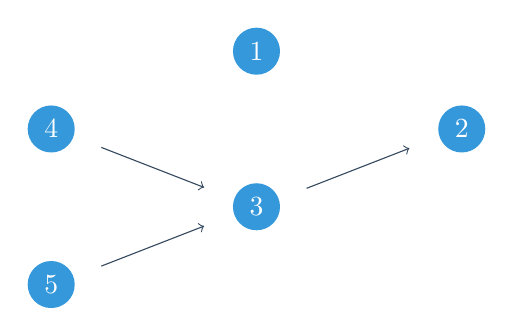
\begin{tikzpicture}[shorten >=1pt,->]
  \tikzstyle{vertex}=[circle,text=white,fill=paperblue,minimum size=17pt,inner sep=0pt]
%%
\pgfsetcolor{papergray}
  % Edge: v1 -> v2
  % \draw [->] (110.89bp,96.315bp) .. controls (119.4bp,93.002bp) and (129.88bp,88.92bp)  .. (148.83bp,81.538bp);
  % Edge: v3 -> v2
  \draw [->] (110.89bp,53.586bp) .. controls (119.4bp,56.899bp) and (129.88bp,60.98bp)  .. (148.83bp,68.362bp);
  % Edge: v4 -> v3
  \draw [->] (36.99bp,68.315bp) .. controls (45.496bp,65.002bp) and (55.978bp,60.92bp)  .. (74.934bp,53.538bp);
  % Edge: v5 -> v3
  \draw [->] (36.99bp,25.586bp) .. controls (45.496bp,28.899bp) and (55.978bp,32.98bp)  .. (74.934bp,40.362bp);
  % Node: v1
  \node[vertex] at (92.851bp,102.95bp) {$1$};
  % Node: v2
  \node[vertex] at (166.75bp,74.95bp) {$2$};
  % Node: v3
  \node[vertex] at (92.851bp,46.95bp) {$3$};
  % Node: v4
  \node[vertex] at (18.95bp,74.95bp) {$4$};
  % Node: v5
  \node[vertex] at (18.95bp,18.95bp) {$5$};
%
\end{tikzpicture}
\caption{Artificial story network.}
\label{fig:example-network}
\end{figure}

The number of incoming edges (i.e.\ the number of stories that select a particular pre-text) is called \emph{in-degree}. I use the notation $d_{in}(i)$ to refer to the in-degree of node $i$. If we apply this terminology to the network in Figure \ref{fig:example-network}, we can observe that node 3 has an in-degree of $d_{in}(3) = 2$, whereas node 2 has an in-degree of 1. $Pr(d_{\text{in}})$ is used to refer to the in-degree distribution of a network. Node 1, 4 and 5 have an in-degree of 0. Node 2 has one incoming link ($d_{in}(2)=1$) and node 3 has two incoming edges. $Pr(d_{\text{in}})$ then represents the probability that a randomly chosen node from the network has a particular in-degree (e.g. $Pr(d_{\text{in}}=1)$ = (number of nodes with $d_{\text{in}}=1$) / (total number of nodes) = 0.2).

A common approach to characterize degree distributions is to fit the parameters of a probability density function. Many real-world networks such as the Word Wide Web network and (scientific) citation networks display a degree distribution with a so-called `heavy tail' in which a large proportion of the nodes have a small degree and only a few yet significant number of nodes are connected to many nodes\autocite{newman:2003}. In some networks the degree of the nodes decays exponentially, whereas in others it follows a power-law:
\begin{equation}\label{eq:powerlaw}
Pr(d) \approx d^{-\alpha}
\end{equation}
where values of the parameter $\alpha$ typically fall in the range $1.5 \leq \alpha \leq 3$\autocite[table II]{newman:2003}. Larger values lead to a faster decay in the probability of nodes with a high degree. To illustrate the effect of the exponent, I show in the left subplot of Figure \ref{fig:lorenz-examples} the complementary cumulative distribution function (ccdf) of four randomly generated degree distributions using different values of $\alpha$. Given that two degree distributions follow a power-law, we can compare the exponents of their distributions. However, as \citeauthor{clauset:2009} have shown, many empirical distributions that appear to follow a power-law, are in fact better described using other heavy-tail distributions such as the log-normal distribution\autocite{clauset:2009}. In this chapter, I apply the techniques developed by \citeauthor{clauset:2009} to characterize the degree distributions of story networks\autocite{clauset:2009}.

\begin{figure}
\centering
\includegraphics[width=\textwidth]{images/lorenz_examples.pdf}
\caption{Left: Complementary cumulative distribution functions of four power-law degree distributions with exponents of $\alpha=2$, $\alpha=2.5$, $\alpha=3$ and $\alpha=4$. Right: Lorenz curves corresponding to these power-law distributions. The dashed line represents a degree distribution that exhibits complete equality of the fraction of nodes over the fraction of degree.}
\label{fig:lorenz-examples}
\end{figure}

Heavy tails of degree distributions represent an uneven spread of edges among nodes. This inequality can be represented using a Lorenz curve which was developed by the economist Max Lorenz for representing wealth inequality in a population. The curve displays the fraction of wealth held by the richest fraction of people in a population. Applied to network degree distributions, the curves represent what fraction of edges is held by what fraction of nodes. If all nodes in a network are connected by the same number of edges, the curve forms a straight line, representing total equality. In the situation where a small fraction of nodes holds a large fraction of edges, the curve displays a steep increase, indicating that the edges are spread unevenly among the nodes. To illustrate the Lorenz curve, I show in the right subplot of Figure \ref{fig:lorenz-examples} the Lorenz curves of the degree distributions that correspond to the power-law exponents in the left subplot. The dashed line represents a degree distribution that exhibits complete equality of the fraction of nodes held by the fraction of edges. The degree distribution generated using $\alpha=2$ displays the strongest form of inequality in which only a small fraction of the nodes (0.2) holds a large fraction of the edges (0.8).

The degree of inequality observed in Lorenz curves can be conveniently summarized using the Gini coefficient $G$. This coefficient can be defined as twice the area between the equidistribution (i.e.\ the dashed line in Figure \ref{fig:lorenz-examples}) and an observed Lorenz curve. $G$ falls in the range $0 \leq G \leq 1$ where larger values indicate a higher degree of inequality. The Lorenz curve corresponding to the degree distribution generated with $\alpha=4$ yields $G=0.22$, whereas the curve corresponding to $\alpha=2$ is summarized by $G=0.77$. An advantage of the Gini coefficient is that it allows us to compare networks of different average degree and size\autocite{Badham:2013}. 


\section{Story Network Analysis}\label{sec:network-analysis}

\begin{sidewaysfigure}
\centering
\includegraphics[width=\textwidth]{images/graphs.pdf}
\caption{Story networks of the collection of chain letters (left network) and ``Red Riding Hood'' retellings (right network). Nodes represent individual stories and edges represent pre-textual relationships between stories. The color gradient (from black via white to red) represents the age of each story.}
\label{fig:network-visualization}
\end{sidewaysfigure}

To construct story networks for the collection of ``Red Riding Hood'' retellings and the collection of chain letters, I employ the \emph{Bootstrap Neighbor Clustering} procedure. Figure \ref{fig:network-visualization} provides a graphical visualization of the two networks. The ``Red Riding Hood'' network consists of $n=427$ nodes and $m=439$ edges. The chain letter network consists of $n=554$ nodes and $m=620$ edges. The color gradient (from black via white to red) in the two networks represents the age of each story. Two important observations can be made from visually inspecting the two networks. First, let us consider the chain letter network. As indicated in the introduction and data section, chain letters are explicitly designed to be replicated and redistributed within a short period of time. To confirm the reliability of the proposed methodology, then, the story network extracted by the \emph{Bootstrap Neighbor Clustering} procedure has to be in accordance with some of our preconceptions about the structure of chain letter story networks. The visualization in Figure \ref{fig:network-visualization} indicates that this appears to be the case: most stories in the network are connected to other stories with a similar color shade, which means that, in the chain letter network, stories predominantly select stories of approximately the same age as potential pre-texts. Interestingly, the second (``Red Riding Hood'') network exhibits a similar pattern, with each story showing a clear preference to select pre-texts with a similar color shade (i.e.\ close temporal proximity). Second, it can be observed that the network derived from ``Red Riding Hood'' retellings has a structure with a few hubs, i.e.\ where three or four stories function as pre-text for a large number of stories (which is represented by the size of the nodes in the networks). The chain letter network, on the other hand, displays a more uniform distribution over which stories function as pre-text, which also is in accordance with our expectations about the structure of chain letter networks (cf.\ Section \ref{sec:networks-introduction}).

In what follows, I will statistically characterize these two observations by carefully studying the in-degree distributions of the two story networks. Accurately characterizing the in-degree distribution of the two networks is a fundamental prerequisite to understand which models of network growth potentially underlie the evolution of the two story networks. A power-law characterization of the in-degree distribution, for example, might be accounted for by models of network growth such as the Preferential Attachment model (cf.\ Section \ref{sec:network-evolution}). Subsequently, I will study the development of the two story networks over time. I compare four models of network growth and analyze their in-degree distributions in relation to those of the two story networks.

\subsection{In-Degree Distribution Analysis}

Figure \ref{fig:degree-fits} plots the cumulative complementary distribution function (ccdf) of the in-degree distributions of the story networks on doubly-logarithmic axes. The plots express the probability of stories with at least in-degree $d_{\text{in}}$, which is denoted as $Pr(D \geq d_{\text{in}})$, where $D$ represents a random variable drawn from the distribution. The plots clearly show that the vast majority of stories have a small in-degree and that only a few stories are selected as pre-text by a large(r) number of stories. 

\begin{figure}[t]
\includegraphics[width=\textwidth]{images/degree-fits.pdf}
\caption{Complementary cumulative in-degree distributions of the two story networks (left: chain letters; right: ``Red Riding Hood''). The plot provides for both distributions the best fit of a power-law, log-normal and exponential model. The power-law and log-normal model both fit the empirical in-degree distribution of ``Red Riding Hood'' well. The chain letter in-degree distribution is best described by means of an exponential model.}
\label{fig:degree-fits}
\end{figure}

To obtain a better understanding of the distributions, I perform the rigorous statistical procedure as described by \citeauthor{clauset:2009} to detect power-law behavior in distributions\autocite{clauset:2009}. In many real-world datasets, the power-law property only applies to the tail of the distribution, i.e.\ for values greater than some minimum value $d_{\text{min}}$. The method proposed by \citeauthor{clauset:2009} estimates a minimum value $d_{\text{min}}$ by comparing the empirical distribution to the theoretical cumulative distribution function (cdf). The method aims to optimize the Kolmogorov-Smirnov statistic $D$ by choosing $d_i$ as the value for $d_{\text{min}}$ for which $D$ is the smallest. \citeauthor{clauset:2009} suggest to test whether a dataset actually follows a power law using a goodness-of-fit test and a bootstrapping procedure\autocite{clauset:2009}. The $p$-value resulting from this test answers the question whether possible differences between the empirical data and the model are significant or not. If $p \simeq 0$, then the model cannot be deemed a plausible fit and other distributions are more appropriate. 

At a significance level of 95\%, we cannot reject the hypothesis that the in-degree distribution of the ``Red Riding Hood'' network is generated by a power-law model: $D=0.048, p > 0.07$. By contrast, the power-law model is not a good fit for the in-degree distribution of the chain letter network ($D=0.09, p = 0.001$). Another way to test for power-law behavior is to directly compare a power-law model to another model, such as a log-normal model via a \emph{likelihood ratio test} $R$\autocite{clauset:2009}. Using the likelihood ratio test, we can assess whether the in-degree distributions are more appropriately described by means of a log-normal or exponential model. The log-normal model fits the chain letter distribution significantly better than the power-law model for the full range of in-degree values ($TS=-4.05, p < 0.0001$). The next step is to compare the log-normal model to an exponential model. The test results are indecisive as to whether a log-normal model is more appropriate than an exponential model ($R=0.079, p > 0.9$). Since a log-normal function has more parameters than an exponential function, it seems reasonable -- for reasons of parsimony -- to characterize the chain-letter in-degree distribution as exponential. Although a log-normal model appears to fit the in-degree distribution of ``Red Riding Hood'' slightly better than a power-law function, the test results suggest that the two models do not perform \emph{significantly} different ($R=-1.52, p > 0.1$).

\begin{figure}
\centering
\includegraphics[width=\textwidth]{images/gini-lorenz.pdf}
\caption{The left subplot displays the Lorenz curve of the chain letter and \emph{Red Riding Hood} story network. The gray striped line represents the equidistribution. The right subplot shows the Gini coefficient $G$ of the in-degree distributions for story networks constructed using $\mu$ in the range $0.1 \leq \mu \leq 1$. It can be observed that the value of $G$ remains relatively stable as we increase the value of $\mu$.}
\label{fig:degree-statistics}
\end{figure}

In the left subplot of Figure \ref{fig:degree-statistics}, I present the Lorenz curves of the two in-degree distributions. The summarizing Gini coefficients of these curves are $G=0.36$ for the chain letter network and $G=0.43$ for ``Red Riding Hood''. Compared to their random counterparts, the story networks exhibit a greater degree of inequality with respect to their in-degree distributions (chain letters: $G_{\text{random}}=0.3$; ``Red Riding Hood'': $G_{\text{random}}=0.28$).\footnote{These random graphs are created by randomly rewiring the edges of the story networks while preserving the time constraint, i.e.\ stories may only link to randomly chosen pre-texts of the same or older age.} The degree of inequality is especially large in the case of ``Red Riding Hood'', suggesting that relatively few stories function as pre-text for many other stories. In the right subplot of Figure \ref{fig:degree-statistics}, I visualize the Gini coefficients $G$ for story networks that were constructed with $0.1 \leq \mu \leq 1$. It can observed that the in-degree distributions display a relatively uneven spread of edges among nodes (i.e.~stories) even for high values of $\mu$. This indicates that the `hubness' of the networks is a stable characteristic and not too much the result of cherry picking a particular value of $\mu$. 


\subsection{Story Network Evolution}\label{sec:network-evolution}

In the previous section, I have shown that the two studied story networks display distinct in-degree distributions. The chain letter network exhibits an in-degree distribution which decays exponentially. The ``Red Riding Hood'' network, by contrast, exhibits a heavy-tail in-degree distribution that fits a power-law or log-normal model reasonably well. Retellings of ``Red Riding Hood'' preferentially link to a small number of stories that are pre-texts of many other retellings. In the present section, I turn to the central question of how these distributions come into being. By carefully studying and comparing the structure and evolution of the two story networks to formal models of network growth, I provide empirical evidence for three major conclusions regarding the formation of story networks. First, I provide empirical evidence that stories preferentially select stories in close temporal proximity, which is indicated by a strong lopsidedness towards smaller time-spans in the time-span distributions of stories and their selected pre-texts. Second, I show that the in-degree distribution of the ``Red Riding Hood'' network is significantly correlated with the age of stories, suggesting that retellings of ``Red Riding Hood'' are affected by a mechanism of preferential attachment in which slightly older versions are preferred to be selected as pre-text(s) in producing a new version. Finally, I show that stories have individual attractiveness values that lessen over time.

The Preferential Attachment (PA) model has proven to be a reliable model to account for heavy-tail degree distributions observed in real-world networks. The model was invented by Derek de Solla Price in the context of citation networks\autocite{price:1976} and simplified and generalized by Albert-László Barabási and Réka Albert to account for undirected networks\autocite{barabasi:1999}. The algorithm generates these networks using an attachment mechanism in which new nodes preferentially link to existing nodes with high (in-)degree. A social network is a classic example in which the mechanism of preferential attachment is at play. In a social network, an edge between two persons $a$ and $b$ exists if $a$ knows $b$ or vice versa. Some persons have many connections and a newcomer to the network is more likely linked to these well-known persons than to persons who are relatively unknown. Similarly, web pages preferentially link to well-known sites, such as Wikipedia, rather than to sites that are less familiar. The mechanism of preferential attachment predicts that the probability of creating a new link between entity $a$ and $b$ is proportional to the number of existing connections of $b$. 

\begin{figure}
\centering
\includegraphics[width=\textwidth]{images/attachment.pdf}
\caption{Kernel density plots of time-span distributions. The plots display the distributions over time-spans for the chain letter network and the network induced for Red Riding Hood. As can observed, both time-span distributions display a strong lopsidedness towards smaller time-spans, which indicates a preference for pre-texts in close temporal proximity.}
\label{fig:time-attachment}
\end{figure}

The consequence of the preferential attachment mechanisms is that nodes that enter the network first will attract more links early on, and will continue to do so. As an explanatory model for story networks, the PA model predicts that stories preferentially select old(er) stories as pre-text rather than new(er) stories. To test this hypothesis, I evaluate for each pair of story and pre-text the time elapsed between their publication dates. Figure \ref{fig:time-attachment} plots the kernel density plots of the time-span distribution for the chain letter network and the ``Red Riding Hood'' network. The time-spans have been normalized to $0 \leq \tau \leq 1$, where $\tau$ represents the normalized time-span between a story and a pre-text. Both plots display strong lopsidedness towards smaller time-spans. Chain letters display an even stronger preference for pre-texts in close temporal proximity (median $\hat{\tau}=0.01$) than the retellings of ``Red Riding Hood'' (median $\hat{\tau}=0.11$). Both time-span distributions run counter the prediction of the PA model that stories are predominantly connected to old(er) stories. 

To obtain more insight into the relation between the in-degree and time-span distributions of the story networks, I test in Figure \ref{fig:correlation-degree-age} for the correlation between in-degree and age. As can be observed from the left subplot and confirmed by a Pearson $\rho$ correlation test, there is no evidence that the in-degree distribution of the chain letter network depends on the age of stories ($\rho=-0.02, p > 0.6)$. However, the in-degree distribution of ``Red Riding Hood'' retellings (right subplot in figure \ref{fig:correlation-degree-age}) is significantly correlated with age ($\rho=0.27, p < 0.0001$). In other words, retellings of ``Red Riding Hood'' do display a preference to select older versions as their pre-text(s). Note, however, that although the correlation is significant, its coefficient is rather low and the relatively low slope of the linear fit suggests that age affects in-degree only in a limited, upper-bounded range.

\begin{figure}
\centering
\subfigure[Chain letters]{\includegraphics[width=0.49\textwidth]{images/letter-time-plot.pdf}}
\subfigure[``Red Riding Hood'']{\includegraphics[width=0.49\textwidth]{images/rrh-time-plot.pdf}}
\caption{Correlation between in-degree and age. The two plots display the correlation between the age of a story and its in-degree for both the chain letter network and the ``Red Riding Hood'' network. The chain letter in-degree distribution does significantly correlate with the age of the letters ($\rho=-0.02, p > 0.6$). The in-degree distribution of the network of ``Red Riding Hood'' is significantly correlated with age ($\rho=0.27, p < 0.0001$).}
\label{fig:correlation-degree-age}
\end{figure} 

To account for the interaction between in-degree and age, I propose a growing network model, which is based on Price's model of preferential attachment~\autocite{price:1976}. In addition to the frequency-based attraction resulting from the preferential attachment mechanism, stories in this new model have individual values of attraction which lessen over time\autocite[Cf.][]{dorogovtsev:2000,eom:2011,Goldberg:2015}. Similar to the preferential attachment algorithm, the model begins with initializing an unconnected network consisting of $m_0$ nodes. At each succeeding time step a single node is added to the network. With a probability $(1 - p)$, a new node connects to $m \leq m_0$ existing nodes with uniform probability. With a probability $p$, the node is connected to $m \leq m_0$ nodes according to the preferential attachment mechanism. The probability to connect to an existing node is given by:
\begin{equation}
p(i) = \frac{\alpha_i \beta_i}{\sum^n_{j=1} \alpha_j \beta_j},
\end{equation}
where $\alpha_i = d_{\text{in}}(i)$ and $\beta_i$ represents the attractiveness of a node at a particular time step. If we set $\beta_i$ to represent a constant value, the model reduces to the original preferential attachment algorithm. Following previous studies\autocite[E.g.][]{eom:2011,Goldberg:2015}, I propose to lessen the attractiveness of a node exponentially over time:\autocite[Eom \& Fortunato add a node's in-degree to its attractiveness at a particular time step. In this study, I choose to weigh a node's in-degree by its attractiveness by \emph{multiplying} the two values. Cf.][]{eom:2011}
\begin{equation}
\beta_i = \beta^i_0 e^{- \tau / \gamma},
\end{equation}
where $\beta^i_0$ represents a node's initial attractiveness and $\tau$ represents the age of a node. The parameter $\gamma$ acts as an ``attention span'' parameter which controls the slope of the exponential decay\autocite{Goldberg:2015}. If $\alpha_i$ is held constant, the model's growth mechanism is restricted to the temporal attractiveness of nodes. Each node $i$ is assigned an individual initial attractiveness value $\beta^i_0$, which is sampled from a symmetric Dirichlet distribution with hyper-parameter $\phi$.\footnote{The choice for sampling from a Dirichlet distribution is largely motivated by the fact that Dirichlet processes are often employed to model data that, like the presented story networks, tend to develop in a `rich get richer' fashion.} Values of $\phi$ between zero and one generally result in a more `peaky' attractiveness distribution, in which only a few nodes are highly attractive. Higher values ($\phi \geq 1)$ result in a more uniform attractiveness distribution. In all experiments, I fix $\phi$ to 0.1. By holding the variable $\alpha_i$ and $\beta_i$ constant, we can analyze the various types of attractiveness in isolation and their interplay. More specifically, I investigate the following four models of network growth:
\begin{enumerate}
\item Preferential Attachment (PA) Model, where $\beta_i = 1$;
\item Temporal Preferential Attachment (T-PA) Model, where $\beta^i_0 = 1$;
\item Temporal Attractiveness (TA) Model, where $\alpha_i = 1$;
\item Preferential Attachment Temporal Attractiveness (PA-TA) Model.
\end{enumerate}

\begin{figure}
\centering
\includegraphics[width=\textwidth]{images/degree-comp.pdf}
\caption{Complementary cumulative in-degree distributions of the empirically derived network and simulations of the PA, T-PA, TA, and PA-TA modes. The left subplot shows the in-degree distribution of the chain letter network. The corresponding distributions of the four growing network models were obtained from a single simulation. The right subplot provides the same information for ``Red Riding Hood''.}
\label{fig:degree-model-comparisons}
\end{figure}

Figure \ref{fig:degree-model-comparisons} presents the complementary cumulative in-degree distributions of both story networks as well as those of the four proposed models. I will compare the in-degree distributions on the basis of their corresponding Gini coefficients $G$, which are presented in Table \ref{tab:gini-comparison}. The four growing network models are probabilistic and therefore results vary from simulation to simulation. The reported Gini coefficients are obtained by averaging 50 simulations. 

The PA model generates heavy-tailed in-degree distributions for ``Red Riding Hood'', of which the summarizing $G$ values are comparable to the empirical coefficient. The Gini coefficient of the chain letter network is much smaller than those produced by the PA model. As was expected, the time-span distributions of the PA model are negatively skewed (chain letters: median $\hat{\tau}= 0.7$; ``Red Riding Hood'': median $\hat{\tau}=0.5$) and the oldest nodes (i.e.\ the nodes that first enter the network) receive most of the incoming links over time. The three growing network models that take the age of nodes into account produce positively skewed time-span distributions in which younger nodes are preferred over older ones (chain letters: T-PA = 0.01, TA = 0.03, PA-TA = 0.04; ``Red Riding Hood'': T-PA = 0.06, TA = 0.07, PA-TA = 0.08). The Gini coefficients of the T-PA model are, however, rather small compared to the empirical coefficients. The temporal attractiveness (TA) model generates in-degree distributions that display the most similar degrees of inequality to those of the chain letter network. In the case of ``Red Riding Hood'', the best results are obtained by the PA-TA model.

\begin{table}
  \centering
  \begin{tabular}{lrrrrr}
  \toprule
                    & \multicolumn{5}{c}{Gini Coefficient}   \\ \midrule
                    & Empirical & PA   & T-PA & TA   & PA-TA \\ \cmidrule(r){2-6}
    Chain letters   & 0.36      & 0.41 & 0.29 & {\bf 0.36} & 0.41  \\
    Red Riding Hood & 0.43      & 0.41 & 0.29 & 0.37 & {\bf 0.43}  \\
  \bottomrule
  \end{tabular}
  \caption{Gini Coefficients of the two story networks (i.e.\ chain letters and ``Red Riding Hood'') and the four growing network models (i.e.\ PA, T-PA, TA, and PA-TA). The reported Gini coefficients are obtained by averaging 50 simulations for each of the four models of network growth. The empirical chain letter network displays an in-degree distribution which is most similar to those generated by the temporal attractiveness (TA) model. The in-degree distribution of the empirical ``Red Riding Hood'' network is most similar to the distributions generated by the Preferential Attachment Temporal Attractiveness (PA-TA) model.}
  \label{tab:gini-comparison}
\end{table}

\section{Discussion}\label{sec:networks-discussion}

In this chapter, I have studied the structure and evolution of story networks. Story networks, defined as non-hierarchical agglomerations of pre-textual relationships, represent streams of retellings in which retellers modify and adapt retellings in a gradual and accumulative way. The first challenge was to develop methods that allow us to automatically extract such story networks from raw text collections. To this end, I have proposed a clustering procedure, termed \emph{Bootstrap Neighbor Clustering}, which approaches the problem of pre-text selection as an open-set problem and attempts to bootstrap pre-textual story networks. I have constructed such story networks for two diachronic collections of retellings: a collection of paper chain letters and a collection of Dutch ``Red Riding Hood'' retellings. 

Using these extracted networks as a base, it was possible to provide a mechanistic understanding of story network growth and, by extension, of retellers' motivations for choosing particular story versions to base their retelling on. I hypothesized that stories are differentially preferred to function as a retelling's pre-text given three types of attractiveness: frequency-based, temporal, and model-based attractiveness. To gain more insight into the relations between stories and their pre-texts, I assessed the patterns of connectivity of the two story networks by performing a rigorous statistical analysis of their in-degree distributions. The in-degree distribution of ``Red Riding Hood'' displays heavy-tail properties that are well characterized by means of a power-law or log-normal model. Such heavy-tailness implies that a large proportion of stories have small in-degree values and only a few, yet significant number of stories function as pre-textual context for a large number of other stories. The heavy-tail distribution of ``Red Riding Hood'' contrasts with the relatively uniform in-degree distribution of the chain letter network, which was characterized as being exponential. 

In addition, I have demonstrated that retellings of chain letters and ``Red Riding Hood'' are published in relatively close temporal proximity. The effect of temporal attractiveness is most strongly observed in the chain letter corpus. Its story network displays a chain-like structure that is reminiscent of the letter's request to be redistributed within a short period of time. It was shown that the time-span distribution of the chain letters does not display a positive correlation with its corresponding in-degree distribution. Retellings of ``Red Riding Hood'', on the other hand, do exhibit a significant correlation between in-degree and age. These contrasting results can be linked to an important difference between the chain letter and ``Red Riding Hood'' retellings: Whereas retellers of ``Red Riding Hood'' can choose from a vast amount of story versions, chain letter retellers are requested to redistribute and retell one specific version. Moreover, it was shown that, in the retelling of chain letters, the mechanism of preferential attachment has no effect.

To explore which mechanisms potentially underlie the evolution of the two story networks, I have investigated a model of network growth. In addition to a preferential attachment mechanism, this model implements a form of model-based attractiveness which decays exponentially in time. The model that incorporates both preferential attachment and temporal attractiveness (PA-TA) best simulates the in-degree distribution of ``Red Riding Hood''. The more parsimonious temporal attractiveness (TA) model sufficed to account for the observed in-degree distribution of the chain letter network. This result concurs with the finding that the in-degree distribution of the chain letter network does not depend on age. Both models of network growth generate positively skewed time-span distributions that are comparable to the observed story network distributions. 

This being said, I wish to stress that there is not one true story network. In this chapter, I made a rather conservative and simplifying choice by investigating pre-textual relationships between stories on the basis of their vocabulary. However, the number of dimensions on which stories can be considered (dis)similar is virtually endless. In order to avoid falling into an `essentialist' trap, future research should first be directed toward studying different dimensions of story similarity (e.g.\ topics, motifs, genre) and their effect on the structure of story networks\autocite[Cf.][]{abello:2012}. A second point of future research is to further explore macroscopic properties of story networks. While the present study mainly focused on the in-degree distributions of story networks, one needs to investigate other general principles governing their structure and evolution in order to obtain a more profound understanding of story networks. Many complex real-world networks can be characterized as so-called `small-world networks', which exhibit two fundamental properties: (i) locally connected groups of nodes and (ii) a short average shortest path length between nodes~\autocite{watts:1998,newman:2003}. I take it to be an interesting question whether story networks display this small-world property. In this scenario, stories would be connected to only a few other stories, while at the same time all stories in the network would be connected to each other through only a few intermediate steps. Another principle governing many real-world networks is a modular structure. Networks with modular structure are hierarchically organized into local groups of densely connected nodes, with a low density of connections \emph{between} groups\autocite{newman:2003}. A modularity analysis of story networks could reveal that stories with high in-degrees function as bridges between local `story communities' and integrate them into a single network\autocite{carron:2012}.
%!TEX root = ../main.tex

\chapter{General Discussion}\label{ch:conclusion}
\markboth{GENERAL DISCUSSION}{} \markright{GENERAL DISCUSSION}

\chapterprecishere{``[Darwin] is no longer the authoritative old man with a beard substituting for God.''}{Gillian Beer}{Darwin's Plots}

\vspace{3.5ex plus 1ex minus .2ex}
\noindent In what preceded, I have offered new perspectives on the mechanisms underlying story transmission and selection. In essence, the approach presented here builds on the insights gained from both folkloristic and literary accounts of story transmission\autocite{stephens_mccallum,boyd:2009,boyd:2010,zipes:2006,zipes:2012,geerts:2014}. However, while such accounts have undoubtedly yielded a wealth of insightful ideas about the mechanisms at play in story transmission, their arguments and claims often remain programmatic and are based on informal verbal arguments that do not allow for rigorous quantitative evaluations. Recent developments in the cultural evolution research program have shown the benefits of employing \emph{formal} models to further the understanding of cultural selection processes. By positioning itself explicitly and extensively in dialog with the cultural evolution research program\autocite{sforzafeldman:1981,boyd_richerson:1985,mesoudi:2011,mesoudi:2015}, the present study aimed to advance our understanding of story transmission processes by means of such formal models of cultural evolution. The added value of the computational approach to story transmission presented in this study is that it yields specific, replicable predictions that can be quantitatively and rigorously evaluated against real-world data. At the same time, it also enables us to isolate and systematically compare forces of selection at play in story transmission. In this concluding chapter, I will synthesize the findings presented in Chapters \ref{ch:motif-classification} to \ref{ch:story-networks} from (i) a methodological perspective that assesses various ways to formally represent stories in order to study real-world story transmission (Research question 1), and (ii) a theorizing perspective that evaluates what the preceding analyses tell us about the factors that determine story transmission and selection (Research question 2--4).

\section[methodological challenges]{Methodological challenges}

While the cultural evolution research program has investigated the mechanisms of story transmission in laboratory contexts\autocite{mesoudiwhiten:2008}, few attempts have been made to apply this framework and encompassing research methods to real-world, historical story data\autocite[Notable exceptions are:][]{tehrani:2013,daSilva:2016}. Therefore, the present study needed to resolve a number of methodological challenges prior to addressing its main research questions. Perhaps the most important methodological issue, which is addressed throughout this entire study, is how stories should be represented in order to computationally study real-world story transmission and selection (Research question 1). As there is no simple `one solution fixes all' answer to this question, I explored a number of different data representations, each of which has potential advantages and disadvantages for studying certain aspects of story transmission. 

In traditional folktale research, the methods used to describe and study relations between stories revolves primarily around the motifs from Thompson's \emph{Motif-Index}\autocite{thompson:1955}. In such studies, motifs are used as the primary descriptive units of stories, and their constellation defines their corresponding tale type as described in, for example, \citeauthor{uther:2004}'s tale type catalog\autocite{uther:2004}. The problem with these traditional approaches is that, in practice, the motifs are not used to identify tale types. Rather, the typical classification strategy in such analyses is an \emph{a priori} assigning of the story under investigation to a single tale type, before any of its motifs are properly identified. As a consequence, the object of investigation is considered solely in light of the motifs that are associated with that particular type. Thus, the classification strategy of predefined tale types and encompassing motifs \emph{encourages} to foreclose particular connections between stories. Neither the concept of a tale type, nor the motifs that supposedly constitute them, is without risk. 

Another problem with tale types and predefined motifs is that they inevitably decontextualize stories. As Marina Warner aptly puts it: the folktale type catalog ``provides a list of ingredients [i.e.\ motifs] and recipes [i.e.\ tale types] with no evocation of their taste or the pleasure of the final dish, nor sense of how or why it was eaten''\autocite[XVIII]{warner:1995}. In other words, stories are torn from their original contexts and might be generalized to a level too abstract to retain any significance. If we, for instance, would analyze the more than four hundred versions of ``Red Riding Hood'' from Chapter \ref{chp:red-riding-hood} in terms of the presence or absence of the motifs listed under tale type ATU 333 ``Little Red Riding Hood'', most versions would become indistinguishable. As such, the motif classification leaves us without means to explain the observed variation and progression through time.

One of the central claims in this study is that tale types should serve the interpretation of actual stories; not the other way around. Tale types can in fact be dangerous when the classification of stories into tale types becomes a static, authoritative, `this or that' enterprise that mutes the many consonant and dissonant resonances with other stories\autocite[Cf.][]{frank:2010}. The potential danger of foregrounding types instead of stories is amplified by Arthur Frank in the context of stories describing experiences of illness:
\begin{quote}
  \noindent ``Typologies risk putting stories in boxes, thus allowing and even encouraging the monological stance that the boxes are more real than the stories, and the types are all that need to be known about the stories. In a world where simplification is a pretext for knowing, and knowing is a pretext for controlling, typologies are risky.''\autocite[118--119]{frank:2010}
\end{quote}
In principle, there is nothing wrong with using tale types as analytical tools, as long as we recognize them to be only one out of many possible perspectives. Typologies invite us to make connections among similar stories, which helps researchers to get a grip on stories and enhance their interpretation. However, when the identification of types becomes a goal in itself, we run the risk of remaining blind to the variation exposed within a category, and of foreclosing both existing and potential relations between stories belonging to separate categories. This risk is anything but trivial if we want to explain how stories are created, interpreted, adapted, and retold. The key or Bakhtinian ``dialogical trick'', as \citeauthor{frank:2010} suggests, is to sustain \emph{openness} and ``[t]ypologies should never be considered final''\autocite[119, 121]{frank:2010} nor should the understanding of which stories fit what tale type.

In contrast with arborescent classification systems which consider tale types to be primary, I advocated an exemplar-based approach of stories. Exemplar-based approaches differ from typology-based approaches in that the object of interest is not the overarching tale type, but lies primarily with the tale `token', i.e.\ the actual story\autocite[119]{frank:2010}. Each story is considered to be a unique entity that is related to other story exemplars in various -- not necessarily predetermined -- ways. In Chapter \ref{ch:story-networks}, I conceptualize the relationships between story exemplars as a network that consists of more and less densely connected clusters of stories. As such, tale types can be considered to be emerging implicitly from highly dense clusters of similar stories. What is considered to be a similarity between stories in the present approach is never static, but depends on the perspective one wishes to take or the image one aims to construct. In Chapter \ref{ch:story-networks}, for example, similarities between stories were determined on the basis of their vocabulary (using a bag-of-words representation), whereas in the study about ``Red Riding Hood'' in Chapter \ref{chp:red-riding-hood}, more abstract perspectives such as `time', `plot' and `irony' contributed to the conceived similarities. Chapter \ref{ch:animacy} presented yet another perspective. To study the factors determining the successfulness of fairy tales from the Brothers Grimm's \emph{Kinder- und Hausmärchen}, I focused on the stories' character cast, which were represented as semantic vectors (i.e.\ word embeddings). In studying story transmission and selection from an evolutionary perspective, it is of utmost importance to acknowledge that relations between stories are malleable and can only be accounted for if we adopt data-driven representations of stories that do not superimpose predefined categories onto stories.

Each of the data-driven representations explored in the present study have certain advantages and disadvantages. First, the character representations employed in Chapter \ref{ch:animacy} have the advantage of conveying semantic information. In addition, these representations require minimal manual labor, which greatly facilitates analyses of large-scale data collections. However, these representations only represent stories on a single dimension (i.e.\ the character cast), and ignore the fact that there are many other dimensions that are (potentially) of equal importance in establishing connections between stories. The bag-of-words representations used in Chapter \ref{ch:story-networks}, by contrast, represent stories on \emph{multiple} dimensions. Bag-of-words representations are powerful, widely used representations, which are computationally efficient and -- even more so than the character representations in Chapter \ref{ch:animacy} -- require minimal manual labor. Despite the fact that bag-of-words make the rather crude simplification of ignoring many higher-order aspects of texts (e.g.\ word order, sentences, structure), they provide effective means to expose important relationships between stories. 

The bag-of-words representations of Chapter \ref{ch:story-networks} contrast sharply with the detailed and fine-grained representations employed in Chapter \ref{chp:red-riding-hood}. The representations in Chapter \ref{chp:red-riding-hood} depend on a rigorous and extensive narratological text analysis consisting of over three hundred questions, which served as the basis for studying the evolution of ``Red Riding Hood'' in a large corpus of Dutch retellings. This questionnaire consists of various questions concerning high- and low-level aspects of the story, ranging from the way characters are named to aspects of theory of mind. While the bag-of-words representations of Chapter \ref{ch:story-networks} also represent stories in a high-dimensional space, the questionnaire approach has the advantage of enabling researchers to represent stories on multiple dimensions with varying degrees of abstraction and detail. The obvious drawback of these representations is, however, that they require labor-intensive and subjective manual analysis (both in the choice for particular questions as well as in the answers given to these questions).

Note that many of the questions employed in Chapter \ref{chp:red-riding-hood} resemble motifs from \citeauthor{thompson:1955}'s \emph{Motif-Index of Folk Literature}\autocite{thompson:1955}, which formed the central representation form of stories in Chapter \ref{ch:motif-classification}. Questions such as ``Is the wolf's belly filled with stones or some other material?''\ or ``Is Red Riding Hood eaten by the wolf?''\ can be linked to, respectively, motifs Q426 (\emph{Wolf cut open and filled with stones as punishment.}) and K2011 (\emph{Wolf poses as ``grandmother'' and kills child.}). Yet, the fact that there are some obvious similarities between some of Thompson's motifs listed under tale type ATU 0333 and some parts of the questionnaire does not imply that the list of motifs and the questionnaire should be considered to be on a par. The questionnaire is to be considered as a data-driven superset of tale type ATU 333 and its constituting motifs. That is to say, the questionnaire entails the given motifs and, at the same time, adds numerous other dimensions of variation on which the stories can be compared. Importantly, these dimensions of comparison (i) arise from the collection of stories under investigation rather than being imposed onto the data and (ii) are never finalized but remain open to reconfiguration and addition when new versions of the story are added to the collection.

\section{Story Transmission and Theory}

Using these data-driven representations, I addressed a number of questions concerning the mechanisms underlying story transmission and selection in Chapters \ref{ch:animacy} to \ref{ch:story-networks}. Chapter \ref{ch:animacy} presented original empirical work that contributes to answering Sperber's fundamental question of how to explain `contagious' culture\autocite{sperber:1996}, or, more specifically, which stories successfully `stick' and what content-based factors determine their successfulness. In particular, I tested the hypothesis of whether a `character bias' (i.e.\ a disposition for particular character types) is at play in the cultural selection of fairy tales (Research question 2). Taking the famous fairy tale collection \emph{Kinder- und Hausmärchen} (1857) by the Brothers Grimm as a case study, I provided empirical evidence for the existence of several character types that affect the successfulness of a story. It was shown that successful fairy tales exhibit a significant preference for (i) characters with names that refer to family relationships, (ii) animal characters and (iii) minimally counterintuitive agents. 

It is interesting to regard these findings in light of previous proposals with respect to the role of characters in story transmission. Recall the epigraph of Chapter \ref{ch:motif-classification}, which recites \citeauthor{thompson:1977} stating that a motif is ``the smallest element in a tale having a power to persist in tradition''.\autocite[415]{thompson:1977} \citeauthor{thompson:1955}'s motifs generally fall into three categories, the first being the tale's characters. These characters, in order to have the power of persistence Thompson attributes to motifs, must exhibit something ``unusual and striking''\autocite[415]{thompson:1977}. Interestingly, these properties typically apply to marvelous creatures such as witches, ogres and fairies, or, in other words, the so-called minimally counterintuitive agents (cf.\ Chapter \ref{ch:animacy}). The present study provides empirical evidence for \citeauthor{thompson:1977}'s hypothesis that such marvelous characters have a power to persist in tradition. At the same time, however, the present study updates Thompson's proposal by showing that minimally counterintuitive agents are not only persisting motifs, but also serve as popularizing \emph{attractors} in the cultural selection of fairy tales. Moreover, the empirical findings of the current study add further support to hypothesized content-based biases in story transmission (e.g.\ a disposition for social information\autocite{reysen:2011,Stubbersfield:2014}). Although these biases have to some extent been investigated through experimental transmission chain studies in the lab\autocite[See, for instance,][]{mesoudi:2006,barrett:2004,Upal:2007,HarmonVukic:2009,Barrett:2009}, the current study presents a unique account in support of these hypotheses on the basis of historical, real-world data. 

Importantly, while current experimental research and research in literary and folkloristic studies primarily focuses on detecting positive biases in story transmission (i.e.\ traits that accrue a story's chances of success), the concept of `negative biases' has been largely overlooked. To address this hiatus in our understanding of story transmission, the current study homed in on the so-called `impopularizing' character types of fairy tales. The results suggested that unsuccessful fairy tales from \emph{Kinder- und Hausmärchen} typically revolve around (i) religious characters, (ii) criminals and hooligans and (iii) generic groups with a rather negative connotation. This negative bias away from stories with generic, indefinite groups ties in with the study on the evolution of ``Red Riding Hood'' (Chapter \ref{chp:red-riding-hood}), in which the wolf has become less generic and more individualized over time. Thus, it would be interesting to further pursue the question of whether these findings are part of a more general development in which individualized stories exhibit a transmission advantage in future research.

The progressive individualization of the wolf is only one of the many transformations that ``Red Riding Hood'' has undergone in the past centuries. While originally intended as a parable intended to warn young ladies of the French court about debonair and sweet-talking rapacious wolfs, ``Red Riding Hood'' has become an increasingly autonomous story and has been subjected to experimentation and reconfiguration. In Chapter \ref{chp:red-riding-hood}, I have systematically and quantitatively investigated this development on the basis of a large longitudinal collection of Dutch retellings of ``Red Riding Hood''. I demonstrated that the development of the story can be characterized as a gradual accumulation of modification: new versions of a story tend to modify and adapt prior retellings, and these prior retellings are published in close temporal proximity to these new versions (Research question 3). The resulting diachronic picture resembles a chain of retellings, in which retellers introduce adaptations and innovations. If these adaptations and innovations are further retold, they may come to gradually replace existing story elements. As such, I have argued, the progressive alteration of ``Red Riding Hood'' in the Netherlands can be interpreted as a cultural evolutionary process.

Finally, the observed preference of authors to produce new versions of ``Red Riding Hood'' on the basis of temporally proximate versions can be interpreted as evidence for a second bias in story transmission (i.e.\ `age bias'). Yet, although this age-dependent selection mechanism for ``Red Riding Hood'' adds important insights to our knowledge about story transmission, it cannot explain why particular story versions versions of approximately the same age are differentially preferred to function as pre-text for new retellings. To address these issues, Chapter \ref{ch:story-networks} further scrutinized this age bias while testing other biases that might function as explanatory models in story transmission (Research question 4). By extensively and systematically comparing outcomes of computational simulations with real-world observations of story transmission, it was shown that story transmission is affected by a positive frequency bias as well as a model-based bias which reduces in strength over time.

The simulations of network growth employed in Chapter \ref{ch:story-networks} represent simplified mathematical models of story transmission. A major theoretical benefit of employing such simulation models is that they call for detailed and replicable definitions. As such, simulation models force researchers to make their theoretical assumptions explicit. Moreover, simulation models also exhibit an interesting degree of simplicity. In the social sciences, the use of such simplified simulation models has often been fiercely criticized for their inability to capture the complex nature of cultural phenomena\autocite{mesoudi:2011}. Yet, I wish to underscore that -- as already pointed out by Mesoudi -- ``the fact that simulations are highly simplified is the very reason for their usefulness''\autocite[326]{mesoudi:2005}. By deliberately keeping the models simple, researchers can easily isolate and manipulate single variables under highly controlled conditions\autocite{mesoudi:2005,mesoudi:2011}. In recent years, the use of evolutionary models has had revolutionary effects across the social sciences\autocite{mesoudi:2015}, and I believe that the application of such models could also lead to a wealth of new insights in folkloristic and literary studies.

\section{An outlook to future research}

Yet, despite the attested descriptive successes we should refrain from rejoicing too much in technological positivism. Comprehensive, in-depth study of the phenomena observed in real-word story transmission processes still faces a number of challenges. Perhaps the biggest challenge is to develop methods to address the relevant questions considering that there is a lack of data. Longitudinal data collections such as the ``Red Riding Hood'' corpus presented in Chapter \ref{chp:red-riding-hood} are virtually non-existent. In an ideal-case scenario, we would be in possession of data collections that specify the exact paths of transmission between individuals and generations, i.e.\ who learns or copies from whom\autocite{kandler:2015}. The rare existing data collections, however, merely represent sparse, incomplete samples of the actual data and none of them provide explicit information about the transmission paths. An additional complication to the matter is that the currently available data only allow us to study the evolution of a small number of individual stories. Making more data available to obtain a more profound understanding of story selection dynamics that transcend those of the individual story would, however, be time-consuming and laborious, and the effort becomes even more impossible to accomplish if we want to broaden the perspective to the comparison of story transmission processes between different cultures.

Given this lack of diachronic data, I consider it to be of crucial importance that we continue to explore different and new methodologies to analyze real-world story transmission. As pointed out by \citeauthor{kandler:2015}, fine-grained individual-level data of cultural change are difficult to obtain, yet many archaeological and anthropological data collections do describe aggregate, population-level outcomes of evolutionary processes.\autocite{kandler:2015} Such outcomes take the form of frequency distributions of variants of a cultural trait at a particular moment in time, or of frequency changes of variants over time. A central question in the cultural evolution program is how such outcomes can be used to explain observed periods of cultural change\autocite{Mesoudi:2009,kandler:2015,kandler:2015b}. For story transmission processes, good examples of population-level outcomes are popularity polls, indices of reprints and bibliographical databases\autocite{koman:2008,joosen:2014}. All of this information is much easier to obtain than large-scale longitudinal full-text corpora, providing us with a useful starting point for addressing the above-mentioned issues. I take it to be an intriguing question how such sparse, population-level data can be used to further identify and map out the underlying acting-forces in story transmission and selection processes.

With the present study, I hope to have revealed and underscored the descriptive and theoretical advantages as well as the further potential of adapting and appropriating computational-evolutionary models to story transmission research. Yet, just as the life span of a story depends on its being picked up and further retold, the continuation of the ideas and models presented above depends on its being adapted and appropriated in new retellings within future research on story transmission, cultural evolution, and folkloristic and literary studies. Hopefully, the present `story' will contribute to ``spark related thoughts, responses, and readings''\autocite[160]{sanders:2006} in retellings to come. 


\backmatter

\addcontentsline{toc}{chapter}{Bibliography}
\printbibheading
\printbibliography[keyword=primary, heading=subbibliography, title={Primary Sources}]
\printbibliography[keyword=secondary, heading=subbibliography, title={Secondary Sources}]

%!TEX root = ../main.tex
%!TEX spellcheck = nl-NL

\chapter*{Samenvatting}\markboth{SAMENVATTING}{} \markright{SAMENVATTING}

\refstepcounter{chapter}
\begin{otherlanguage}{dutch}
\noindent \emph{Retelling Stories} is een onderzoek naar mechanismes die ten grondslag liggen aan de verspreiding en verandering van (volks)verhalen. Een van de centrale vragen in dit onderzoek is of verhaaltransmissie begrepen kan worden als een cultureel evolutionair process en welke evolutionaire mechanismen daarbij een rol spelen. Om deze vraag te beantwoorden, zoekt deze studie aansluiting bij onderzoek naar computationele modellen van culturele verandering~\autocite[Zie bijvoorbeeld:][]{sforzafeldman:1981,boyd_richerson:1985,mesoudi:2011,mesoudi:2015}. Door gebruik te maken van deze computationele benadering van culturele verandering, probeert de huidige studie om diachrone verhaalontwikkelingen op een kwantitatieve en formele manier te bestuderen en te karakteriseren. Hoewel een computationeel-evolutionaire benadering van verhaaltransmissie (en de daarbijhorende methodologische vraagstukken) centraal staat, gaat deze studie ook de dialoog aan met \emph{kwalitatieve} benaderingen van verhaaltransmissie~\autocite[Zie bijvoorbeeld:][]{stephens_mccallum,boyd:2009,boyd:2010,zipes:2006,zipes:2012,geerts:2014} met als doel de synthese tussen culturele evolutie, (jeugd)literatuur en verhaalonderzoek te versterken. Na een inleidend hoofdstuk, waarin het methodologische kader en de probleemstelling van de studie worden gepresenteerd, wordt in de daaropvolgende vier hoofdstukken een evenredig aantal onderzoeksvragen behandeld, waarvan de onderzoeksrelevantie zowel methodologisch als theoretisch van aard is.  

De eerste onderzoeksvraag vormt het methodologische fundament van de studie en richt zich op de representatie en formalisatie van verhalen om historische verhaaltransmissie en -selectie computationeel te kunnen bestuderen. In hoofdstuk \ref{ch:motif-classification} tot en met \ref{ch:story-networks} worden vier verschillende datarepresentaties onderzocht, die elk potentiële voor- en nadelen hebben voor de bestudering van bepaalde aspecten van verhaaltransmissie. Hoofdstuk \ref{ch:motif-classification} presenteert een `klassieke' representatie van verhalen die gebaseerd is op de beroemde \emph{Motif-Index} ontwikkeld door Stith Thompson\autocite{thompson:1955}. In deze representatie worden motieven beschouwd als de primaire bouwstenen van verhalen en hun verzameling bepaalt tot welk verhaaltype een verhaal behoort (zoals de verhaaltypes in \emph{The Types of International Folktales}\autocite{uther:2004}). Deze representatie, waarin verhalen primair worden beschouwd als instantiaties van bepaalde verhaaltypes, staat haaks op de data-gedreven representaties van verhalen in de hoofdstukken \ref{ch:animacy} tot en met \ref{ch:story-networks}. In deze hoofdstukken worden drie representaties voorgesteld waarin niet het verhaaltype het primaire onderwerp van studie is, maar het eigenlijke verhaal of `verhaal\emph{token}'. Een belangrijk voordeel van deze token-gebaseerde representaties ten opzichte van de `klassieke', type-gebaseerde representatie, is dat overeenkomsten tussen verhalen niet statisch zijn, maar afhankelijk van het door de onderzoeker gekozen perspectief. 

In hoofdstuk \ref{ch:animacy} tot en met \ref{ch:story-networks} worden de data-gedreven verhaalrepresentaties gebruikt om een aantal onderzoeksvragen te beantwoorden over mechanismes van verhaaltransmissie. Hoofdstuk \ref{ch:animacy} levert een bijdrage aan het beantwoorden van de fundamentele vraag hoe `besmettelijke' cultuur verklaard kan worden\autocite[Vergelijk:][]{sperber:1996} door te onderzoeken welke type(s) verhalen beklijven en welke \emph{verhaalinhoudelijke} factoren hierop van invloed zijn (onderzoeksvraag 2). De resultaten laten zien dat de (im)populariteit van sprookjes in sterke mate beïnvloed wordt door het type personages dat in de verhalen voorkomt. Zo hebben populaire, beklijvende verhalen een significante voorkeur voor personages uit de familiesfeer en personages die `minimaal tegenintuïtief' genoemd kunnen worden~\autocite[Zie bijvoorbeeld][]{Barrett:2009}. Impopulaire verhalen, daarentegen, kenmerken zich door bijvoorbeeld het opvoeren van generieke (vaak negatief geëvalueerde) personagegroepen en personages uit de religieuze sfeer.

Na dit hoofdstuk over verhaalinhoudelijke factoren van (on)\-succesvolle verhaaltransmissie volgen twee hoofdstukken over sociaal-geïnformeerde, \emph{context-gebaseerde} processen die ten grondslag liggen aan verhaaltransmissie. Het doel van hoofdstuk \ref{chp:red-riding-hood} is om een beter begrip te ontwikkelen over de processen waarmee kinderverhalen worden herverteld. Het hoofdstuk probeert een antwoord te geven op de derde onderzoeksvraag van deze dissertatie en onderzoekt of de diachrone ontwikkeling van ``Roodkapje'' in het Nederlandse taalgebied gekarakteriseerd kan worden als een (Darwiniaans) evolutieproces, waarin aanpassingen van het verhaal geleidelijk opeengestapeld worden en nieuwe varianten van het verhaal afgeleid zijn van versies uit het recente verleden. Uit de resultaten blijkt dat nieuwe Nederlandse hervertellingen van ``Roodkapje'' inderdaad onderworpen zijn aan leeftijdsafhankelijke selectieprocessen (vergelijkbaar met modetrends). Dat betekent `jonge' vertellingen de voorkeur krijgen om een nieuwe vertelling op te baseren.

Hoewel de leeftijdsafhankelijke selectiemechanismen voor ``Roodkapje'' belangrijke inzichten toevoegen aan onze kennis over verhaaltransmissie, biedt het nog geen verklaring voor de vraag waarom specifieke verhaalversies worden verkozen boven andere versies van ongeveer dezelfde leeftijd om een nieuwe hervertelling op te baseren. Om deze vraag te onderzoeken, neemt hoofdstuk \ref{ch:story-networks} de leeftijdsafhankelijke selectievoorkeur verder onder de loep en onderzoekt daarnaast welke andere selectievoorkeuren een rol spelen in verhaaltransmissie (onderzoeksvraag 4). De resultaten van een systematische vergelijking tussen computationele simulaties met empirische observaties van verhaaltransmissie laten zien dat de differentiële selectie van verhalen sterk beïnvloed wordt door de interactie van een drietal factoren: (i) een frequentievoorkeur (waarbij hervertellers kiezen voor populaire verhalen), (ii) een `modelvoorkeur' (waarbij hervertellers zich laten leiden door bijvoorbeeld de prestige van een auteur of uitgave) en (iii) de eerder besproken leeftijdsvoorkeur. 

\end{otherlanguage}
\addcontentsline{toc}{chapter}{Samenvatting}
%!TEX root = ../main.tex

\chapter*{Summary}\markboth{SUMMARY}{} \markright{SUMMARY}

\refstepcounter{chapter}
\noindent \emph{Retelling Stories} is a study about the mechanisms underlying story transmission and selection. A central question of the study is whether story transmission can be understood as -- and hence should be described as -- a cultural evolutionary process, and which evolutionary mechanisms can be identified in story transmission. To address this question, the approach presented in this study draws inspiration from research on computational models of cultural evolution~\autocite[E.g.][]{sforzafeldman:1981,boyd_richerson:1985,mesoudi:2011,mesoudi:2015}. By positioning itself explicitly and extensively in dialog with this cultural evolution research program, the current study aims to advance our understanding of story transmission processes by formally and quantitatively characterizing diachronic story developments. While its central focus is to provide a computational-evolutionary approach to story transmission (and encompassing methodological challenges), the study also builds on insights gained from both folkloristic and literary accounts of story transmission\autocite[E.g.][]{stephens_mccallum,boyd:2009,boyd:2010,zipes:2006,zipes:2012,geerts:2014}. As such, this study contributes to the further synthesis of the disciplines of cultural evolution, literary theory and folklore. After presenting the methodological framework and problem statement in Chapter \ref{ch:introduction}, the subsequent four chapters address a number of research questions regarding both methodological and theoretical issues of story transmission.

The first research question constitutes the methodological base of the study and addresses the question of how stories should be formally represented in order to study real-world story transmission with computational means. Chapters \ref{ch:motif-classification} to \ref{ch:story-networks} present four different data representations, each of which has potential (dis)advantages for studying particular aspects of story transmission. In Chapter \ref{ch:motif-classification}, a `classical' representation is employed, which is based on the seminal \emph{Motif-Index} developed by Stith Thompson~\autocite{thompson:1955}. In this representation, motifs are considered to be the basic building blocks of stories, and their constellation defines the story type of a story (e.g.\ story types from \emph{The Types of International Folktales}\autocite{uther:2004}). This story representation, in which stories are primarily considered to be mere instances of story types, contrasts sharply with the data-driven story representations proposed in chapters \ref{ch:animacy} to \ref{ch:story-networks}. These chapters present three different story representations, in which the object of interest is not the overarching story type, but lies primarily with the tale `token', i.e.\ the actual story. Crucially, the main methodological and theoretical advantage of these data-driven representations is that what is considered to be a similarity between stories is never static, but depends on the perspective one wishes to take or the image one aims to construct.

Using the exemplar-based story representations, chapters \ref{ch:animacy} to \ref{ch:story-networks} address a number of questions concerning mechanisms underlying story transmission. Chapter \ref{ch:animacy} contributes to answering the fundamental question of how to explain `contagious' culture~\autocite[Cf.][]{sperber:1996} by investigating which stories `stick' and what \emph{content}-based factors determine their successfulness (Research question 2). Taking the famous fairy tale collection \emph{Kinder- und Hausmärchen} as a case, empirical evidence was given for the existence of a number of character types that affect the popularity of a story. Successful, sticky stories exhibit a significant preference for, for instance, characters referring to family relationships and `minimally counterintuitive' agents~\autocite[See e.g.][]{Barrett:2009}. Unsuccessful stories, by contrast, typically revolve around religious characters and generic groups with rather negative connotations.

Subsequent to this chapter on content-based factors of (un)successful story transmission, the remaining two chapters (\ref{chp:red-riding-hood} and \ref{ch:story-networks}) focus on socially informed, \emph{context}-based processes that underlie story transmission. The goal of Chapter \ref{chp:red-riding-hood} is to enhance our understanding of the processes through which children's stories are retold. The chapter aims to answer the third research question of this thesis and investigates whether the diachronic development of ``Red Riding Hood'' in the Netherlands can be characterized as an (Darwinian) evolutionary process. It is shown that the evolution of the story can be characterized as a `gradual accumulation of modification' in which new versions of ``Red Riding Hood'' tend to modify and adapt prior retellings, and these prior retellings are published in close temporal proximity to these new versions (Research question 3). 

The observed disposition of authors for temporally proximate stories to produce new retellings can be interpreted as an `age bias' in story transmission, comparable to fashion trends or fads. Yet, although the presence of age-dependent selection mechanisms adds important knowledge to our understanding of story transmission processes, it cannot explain why certain story versions of approximately the same age are differentially preferred to function as a story's pre-text. To address this issue, Chapter \ref{ch:story-networks} further scrutinizes the age-dependent selection mechanism while testing and evaluating other biases that could serve as explanatory models for story transmission (Research question 4). On the basis of an extensive and systematic comparison between the output of computational simulations and empirical observations of story transmission, it is shown that the differential selection of stories is affected by the interplay of three biases: (i) a positive frequency bias (in which retellers prefer frequently retold stories), (ii) a model-based bias (e.g. author prestige), and (iii) the aforementioned age bias. 

\addcontentsline{toc}{chapter}{Summary}
%!TEX root = ../main.tex

\chapter*{Curriculum Vitae}

\noindent Folgert Karsdorp was born in Leidschendam, the Netherlands, on the 3rd of November, 1983. He studied Dutch Language \& Culture at Leiden University for which he received his BA in 2007. Subsequently, he studied the research master Linguistics at the same university and obtained his MA in 2009. After working for a year as a research assistant at the Freie Universität Berlin, Karsdorp worked as a (computational) linguist at the Institute for Dutch Lexicology until December 2011. In 2012, he started working as a Ph.D candidate in the Tunes \& Tales project at the Meertens Instituut in Amsterdam, which was funded by the Royal Dutch Academy of Arts and Sciences. In April 2016, Karsdorp acquired a research assistant position at the Centre for Language Studies of the Radboud University in Nijmegen. At present, Karsdorp is employed as a postdoctoral researcher at the Meertens Instituut in Amsterdam.
\clearpage

\end{document}